% !BIB TS-program = biber
% !TeX spellcheck = <en EN>
%%%% Modèle proposé par colin.avogadri@umontpellier.fr %%%%
%%%% 3 Février 2022 %%%%

\documentclass[english,12pt,a4paper]{book}

\usepackage[utf8]{inputenc}
\usepackage{mathpazo}
\usepackage[semibold]{sourcesanspro}
% \usepackage{sectsty}
% \allsectionsfont{\sffamily}
\usepackage[T1]{fontenc}
\usepackage[english]{babel}
\usepackage{amsmath}
\usepackage{amsfonts}
\usepackage{fancyhdr}
\usepackage{amssymb}
\usepackage{xcolor}
\usepackage{csquotes}
% \usepackage{color} % où xcolor selon l'installation
\definecolor{Valentia}{RGB}{233,78,82}
\definecolor{Titleblue}{RGB}{114, 146, 162}
\usepackage{mdframed}
\usepackage{multirow} %% Pour mettre un texte sur plusieurs rangées
\usepackage{multicol} %% Pour mettre un texte sur plusieurs colonnes
\usepackage{scrextend} % Forcer la 4eme  de couverture en page pair
\usepackage{tikz}
\usepackage{graphicx}
\usepackage[absolute]{textpos} 
\usepackage{colortbl}
\usepackage{array}
\usepackage{hyperref} 
\usepackage{microtype}
\usepackage{easyReview}
\usepackage{framed}
\usepackage{latexsym}
\usepackage{url}
\definecolor{newcolor}{rgb}{.8,.349,.1}
\usepackage{subcaption}
\usepackage{stackengine}
\usepackage{svg}
\usepackage{wrapfig}
\usepackage{pdflscape}
\usepackage{afterpage}
\usepackage{capt-of}
\usepackage{longtable}
\usepackage{makecell}
\usepackage{titlesec}
\usepackage{float}
\usepackage{booktabs}
\usepackage{tabularx}
\usepackage{siunitx}
%\usepackage{breqn}
\usepackage{bookmark}
\usepackage{etoc}
% \usepackage{minitoc}
\usepackage[export]{adjustbox}
\usepackage{etoolbox}
\usepackage{letltxmacro}
\usepackage{xparse}
\usepackage{listings}
\usepackage{xstring}
\usepackage{ifthen}
\usepackage[toc,page]{appendix}
\usepackage[toc, acronym]{glossaries}
\usepackage{upgreek}
% \usepackage{textgreek}
\usepackage[minimal=true]{chemmacros}
\usepackage{indentfirst}

\usepackage[backend=biber, backref=true, style=apa, uniquelist=true, maxcitenames=1, uniquename=false]{biblatex} 
% backref: add link in the references to go back up
% uniquelist: write "et al." even if the reference can be ambiguous with only first author name
% maxcitenames: Yeah... not sure...
% uniquename: if true and multiple authors have the same last name, the first name initial is added. When dealing with diacritics (accents, cedilles, etc.), it often think that two references have different authors.

\usepackage{geometry}
% \usepackage[left=1.5in, right=1.5in]{geometry}
% \usepackage[showframe]{geometry} %just to visualise the borders
% \usepackage{refcheck} % See if some references are missing or if Ids are wrong
\usepackage[capitalise,noabbrev]{cleveref}
\zzcommand{\R}{\mathbb{R}}
\zzcommand{\N}{\mathbb{N}}
\zzcommand{\C}{\mathbb{C}}
\zzcommand{\Z}{\mathbb{Z}}
\zzcommand{\norm}[1]{\left\lVert #1 \right\rVert}

\zzcommand{\material}{\mathcal{M}}

\zzcommand{\mass}{m}
\zzcommand{\velFactor}{\nu}
\zzcommand{\decay}{k}
\zzcommand{\diffusion}{D}
\zzcommand{\growthRate}{\gamma}
\zzcommand{\fittingFunc}{\Gamma}
\zzcommand{\fittingFuncObj}{\fittingFunc_{obj}}

\zzcommand{\Water}{\mathcal{W}}
\zzcommand{\Wuser}{\Water_\text{user}}
\zzcommand{\Wsimu}{\Water_\text{simulation}}
\zzcommand{\Wobj}{\Water_\text{objects}}

\zzcommand{\terrain}{\mathcal{T}}
\zzcommand{\height}{\mathcal{H}}
\zzcommand{\depth}{\mathcal{D}}
\zzcommand{\objects}{\mathcal{O}}
\zzcommand{\environment}{\mathcal{E}}
\zzcommand{\Wlevel}{\mathcal{L}}
\zzcommand{\events}{\text{events}}

\zzcommand{\availableObjects}{\Tilde{\objects}}

\zzcommand{\tEvent}{t_e}

\zzcommand{\eps}{\varepsilon}


\zzcommand{\erosionRate}{ \varepsilon }
\zzcommand{\shearStress}{ \tau }
\zzcommand{\shearRate}{\theta}
\zzcommand{\criticalShearStress}{ \shearStress_\text{critical} }
\zzcommand{\velocity}{ \upsilon }
\zzcommand{\capacity}{ C }
\zzcommand{\maxCapacity}{ \capacity_\text{max} }
\zzcommand{\density}{ \rho }
\zzcommand{\particleDensity}{ \density_\text{particle} }
\zzcommand{\soilDensity}{ \density_\text{sediment} }
\zzcommand{\particleMass}{ \mass_\text{particle} }
\zzcommand{\depositionRate}{ \omega } % Not the good notation, but I don't think there is a real notation
% \zzcommand{\real}{ \mathbb{R} }
\zzcommand{\shearStressConstant}{ K }
\zzcommand{\erosionStrength}{ K_{\erosionRate} }
\zzcommand{\particleSize}{ R }
\zzcommand{\settlingVelocity}{ w_s }
\zzcommand{\fluid}{ \text{fluid} }
\zzcommand{\fluidDensity}{ \density_\fluid }
\zzcommand{\fluidVelocity}{ \velocity_\fluid }
% \zzcommand{\buoyancy}{ B }
% \zzcommand{\gravity}{ G }
\zzcommand{\erosionAmount}{ q_\text{detachment} }
\zzcommand{\depositAmount}{ q_\text{deposit} }
\zzcommand{\totalErosion}{ Q }
\zzcommand{\extForce}{ \vec F_\text{ext} }
\zzcommand{\capacityFactor}{ C_\text{factor} }


\zzcommand{\area}{a}
\zzcommand{\Area}{A}
\zzcommand{\length}{l}
\zzcommand{\Length}{L}
\zzcommand{\energy}{E}
\zzcommand{\Einternal}{\energy_{\text{internal}}}
\zzcommand{\Eexternal}{\energy_{\text{external}}}
\zzcommand{\Eshape}{\energy_{\text{shape}}}
% \zzcommand{\time}{t}
\zzcommand{\curve}{C}
\zzcommand{\absorption}{A}
\zzcommand{\deposition}{D}
\zzcommand{\p}{\textbf{p}}
\zzcommand{\q}{\textbf{q}}
\zzcommand{\domain}{\Omega}
\zzcommand{\warp}{\omega}
\zzcommand{\force}{\textbf{F}}
\zzcommand{\influence}{\lambda}
\zzcommand{\windVelocity}{\velocity_{\text{wind}}}
\zzcommand{\std}{\sigma}
\zzcommand{\temperature}{T}
\zzcommand{\dirac}{\delta}
\zzcommand{\identity}{\textbf{I}}

\zzcommand{\heightmap}{H}
\zzcommand{\implicit}{I}
\zzcommand{\densityVox}{DV}
\zzcommand{\binaryVox}{BV}

\zzcommand{\volume}{V}
\zzcommand{\gravity}{\vec g}
\zzcommand{\gravityForce}{\vec F_{\text{gravity}}}
\zzcommand{\buoyancyForce}{\vec F_{\text{buoyancy}}}
\zzcommand{\constGravity}{G}
\zzcommand{\viscosity}{\mu}

\zzcommand{\radius}{r}
\zzcommand{\Radius}{R}

\zzcommand{\noise}{\eta}

\zzcommand{\Esnake}{E_{\text{snake}}}
\zzcommand{\Eintern}{E_{\text{internal}}}
\zzcommand{\Eextern}{E_{\text{external}}}
\zzcommand{\Econt}{E_{\text{continuity}}}
\zzcommand{\Eimage}{E_{\text{image}}}
\zzcommand{\Ecurv}{E_{\text{curvature}}}




% \newdualentry[glossary-options][abbrev. options]{key}{abbr}{Full name}{Description}{Plural (opt)}
\newdualentry[][]{EnvObj}{STE}{Semantic Terrain Entity}{Geographic feature represented sparsly which describe a landscape. We represent it with a \gloss{Skeleton}, \glosses{GenRule} and \glosses{EnvMat}. }{Semantic Terrain Entities}
\newdualentry[][]{EnvVal}{}{environmental attribute}{Value of a geographic field at one point in space and time. }
\newdualentry[][]{EnvMat}{}{environmental modifier}{Description of a modification of a \gloss{EnvVal} around a \gloss{EnvObj}. It can represent the spread or the absorption of material around it, or the deformation of water currents. }
\newdualentry[][]{GeoEvent}{}{geomorphic event}{Modification of a \gloss{EnvVal} in an interval of time with or without spatial bounds. }
\newdualentry[][]{Skeleton}{}{skeleton}{Simplified shape of a \gloss{EnvObj}, as it could be symbolized in a map: as a point, a curve or a region. }
\newdualentry[][]{GenRule}{}{generation rule}{Composed of a \gloss{FitnessFunc} and \gloss{FittingFunc}, the optimisation of the \gloss{GenRule} of an \gloss{EnvObj} through the maximization of its components describe where and how new elements can be added to a semantic terrain. }
\newdualentry[][]{FitnessFunc}{}{fitness function}{Function affected to a \gloss{EnvObj} that, given the \gloss{EnvVal} at a $(x, y)$ position in the space, returns a score describing how well this \gloss{EnvObj} may survive. }
\newdualentry[][]{FittingFunc}{}{skeleton fitting function}{Function affected to a \gloss{EnvObj} that, given the local \gloss{EnvVal} and the shape of the skeleton of the \gloss{EnvObj}, returns a score describing how well this \gloss{EnvObj} fits. It may be seen as a refinement of the \gloss{FitnessFunc}. }
\newdualentry[][]{SteadyState}{}{steady state}{A system is at steady state when internal properties do not change overtime once a dynamic equilibrium has been reached. The \glosses{EnvMat} emission from \glosses{EnvObj} can be seen as a thermodynamic system which achieve thermodynamic equilibrium over time. }

%Intro
\newdualentry[][]{ParamSpace}{}{parameter space}{Set of adjustable parameters that can be modified to control and influence the generation process of content or assets. These parameters can include properties like size, shape, density, or other relevant factors, depending on the specific procedural algorithm being used. By adjusting these parameters, creators can achieve a wide variety of outcomes and patterns, enabling the generation of diverse and customizable content such as textures, levels, or 3D models.}
\newdualentry[][]{LOD}{LoD}{level of detail}{Amount of graphical data or information displayed in a scene or image. Higher LOD means more detail, while lower LOD means less detail. This concept helps manage computational resources, where less important or distant objects have lower LOD to improve performance.}
\def\zzcommand#1{\let#1\undefined\newcommand#1}

\makeatletter
\LetLtxMacro\OldSection\section
\DeclareRobustCommand{\section}{%
  \@ifstar{\sectionstar}{\sectionnostar}%
}
\zzcommand{\sectionnostar}[1]{%
  \begingroup
  \zzcommand{\inheading}{}%
  \OldSection{#1}
  \endgroup
}
\zzcommand{\sectionstar}[1]{%
    \begingroup
    \zzcommand{\inheading}{}%
    \OldSection*{#1}
    \endgroup
}
\makeatother

\makeatletter
\LetLtxMacro\OldSubsection\subsection
\DeclareRobustCommand{\subsection}{%
  \@ifstar{\Subsectionstar}{\Subsectionnostar}%
}
\zzcommand{\Subsectionnostar}[1]{%
  \begingroup
  \zzcommand{\inheading}{}%
  \OldSubsection{#1}
  \endgroup
}
\zzcommand{\Subsectionstar}[1]{%
    \begingroup
    \zzcommand{\inheading}{}%
    \OldSubsection*{#1}
    \endgroup
}
\makeatother

\makeatletter
\LetLtxMacro\OldSubsubsection\subsubsection
\DeclareRobustCommand{\subsubsection}{%
  \@ifstar{\Subsubsectionstar}{\Subsubsectionnostar}%
}
\zzcommand{\Subsubsectionnostar}[1]{%
  \begingroup
  \zzcommand{\inheading}{}%
  \OldSubsubsection{#1}
  \endgroup
}
\zzcommand{\Subsubsectionstar}[1]{%
    \begingroup
    \zzcommand{\inheading}{}%
    \OldSubsubsection*{#1}
    \endgroup
}
\makeatother

% \let\oldsection\section
% \renewcommand{\section}[1]{%
%   \begingroup
%   \newcommand{\inheadingcontext}{}%
%   \oldsection{TEST2}%
%   \endgroup
% }
% \renewcommand{\section*}[1]{%
%   \begingroup
%   \newcommand{\inheadingcontext}{}%
%   \oldsectionstar{TEST}%
%   \endgroup
% }


\LetLtxMacro{\Oldincludegraphics}{\includegraphics}
\RenewDocumentCommand{\includegraphics}{O{} m}{%
	\begin{adjustbox}{max width=\textwidth, max height=\textheight-5\baselineskip}
	    \Oldincludegraphics[#1]{#2}
	\end{adjustbox}
}
\newcommand{\inset}[3][0.2\linewidth]{
    \noindent\stackinset{r}{0.1cm}{b}{0.1cm}{
        \colorbox{white}{
            \includegraphics[width=#1]{#3}
        }
    }
	{\includegraphics{#2}}
}

\newcommand{\teaser}[1]{
    \begin{figure*}
        #1
    \end{figure*}
}

\def\minitoc{
	\etocsettocstyle{\section*{\contentsname}}{}
	\localtableofcontents
	\noindent\textbf{\hyperlink{tocpage}{Back to summary}}
}
% \makeatletter\@addtoreset{chapter}{part}\makeatother%

\sisetup{product-units=repeat}

\emergencystretch=1em

% \setkeys{Gin}{width=\linewidth}

\renewcommand{\cellalign}{cl}
\newcolumntype{H}{>{\setbox0=\hbox\bgroup}c<{\egroup}@{}}

\DeclareCiteCommand{\cite}[\mkbibparens]
  {\usebibmacro{prenote}\usebibmacro{cite:init}}
  {\usebibmacro{citeindex}
   \printtext[bibhyperref]{\usebibmacro{cite}}}
  {\multicitedelim}
  {\usebibmacro{postnote}}

\newbibmacro*{citefullbody}{
  \printnames{labelname}
  \setunit{\addcomma\space}
  \textit{\printfield[]{title}} % remove quotes
  % \textit{\printfield[citetitle]{title}}
  % \setunit{\nameyeardelim}
  (\printfield{year})
}

\DeclareCiteCommand{\citep}
{\usebibmacro{prenote}\usebibmacro{cite:init}}
{\usebibmacro{citeindex}
 \printtext[bibhyperref]{\usebibmacro{citefullbody}}}
{\multicitedelim}
{\usebibmacro{postnote}}

\AtEveryBibitem{\clearfield{url}}
\AtEveryBibitem{\clearfield{note}} % Notes from Mendeley

\lstset {
    language=C++,
    backgroundcolor=\color{black!5}, % set backgroundcolor
    basicstyle=\footnotesize,% basic font setting
}

\makeglossaries
\DeclareDocumentCommand{\newdualentry}{ O{} O{} m m m m g } {
    \newglossaryentry{gls-#3}{
        name={#5},
        text={#5\if\relax\detokenize{#4}\relax\else\glsadd{#3}\fi},
        plural={\IfValueTF{#7}{#7}{#5s}},
        longplural={\IfValueTF{#7}{#7}{#5s}},
        description={#6},
        #1
    }
    \if\relax\detokenize{#4}\relax
    % nothing
  \else
    \newacronym[longplural={\IfValueTF{#7}{#7}{#5s}}, 
        see={[Glossary:]{gls-#3}},
        #2]{#3}{#4}{#5\glsadd{gls-#3}}
  \fi
    \makeglossaries
}



\zzcommand{\gloss}[1]{\ifglsentryexists{gls-#1}{\glsentryname{gls-#1}\ifcsdef{inheading}{}{{\glsadd{gls-#1}}}}{[XXXX]}}
\zzcommand{\glosses}[1]{\ifglsentryexists{gls-#1}{\glsentrylongpl{gls-#1}\ifcsdef{inheading}{}{{\glsadd{gls-#1}}}}{[XXXX]}}
\zzcommand{\Gloss}[1]{\ifglsentryexists{gls-#1}{\Glsentryname{gls-#1}\ifcsdef{inheading}{}{{\glsadd{gls-#1}}}}{[XXXX]}}
\zzcommand{\Glosses}[1]{\ifglsentryexists{gls-#1}{\Glsentrylongpl{gls-#1}\ifcsdef{inheading}{}{{\glsadd{gls-#1}}}}{[XXXX]}}
\zzcommand{\glsnamefont}[1]{\makefirstuc{#1}}



% \zzcommand{\gloss}[1]{\glsentryname{gls-#1}} % \ifcsdef{inheading}{\glsentryname{gls-#1}}{\ifglsentryexists{#1}{\gls{#1}\glsadd{gls-#1}}{\gls{gls-#1}}}}
% \zzcommand{\glosses}[1]{\glsentrylongpl{gls-#1}} % \ifcsdef{inheading}{\glsentrylongpl{gls-#1}}{\ifglsentryexists{#1}{\glspl{#1}\glsadd{gls-#1}}{\glspl{gls-#1}}}}
% \zzcommand{\Gloss}[1]{\Glsentryname{gls-#1}} % \ifcsdef{inheading}{\Glsentryname{gls-#1}}{\ifglsentryexists{#1}{\Gls{#1}\glsadd{gls-#1}}{\Gls{gls-#1}}}}
% \zzcommand{\Glosses}[1]{\Glsentrylongpl{gls-#1}} % \ifcsdef{inheading}{\Glsentrylongpl{gls-#1}}{\ifglsentryexists{#1}{\Glspl{#1}\glsadd{gls-#1}}{\Glspl{gls-#1}}}}
% \zzcommand{\glsnamefont}[1]{\makefirstuc{#1}}

% \let\oldchapter\chapter
% \renewcommand{\chapter}[1]{
%   \begingroup
%   \newcommand{\inheading}{}
%   \oldchapter{#1}
%   \endgroup
% }

\let\ref=\cref
\let\eqref=\cref

\zzcommand{\to}{\mapsto}

% \bibliography{references_terrain}
\addbibresource{references_terrain.bib}


\usepackage[Sonny]{fncychap} %% Pour changer le style de chapitre
\pagestyle{fancy}
%\fancyhf{}
%\fancyhead[RE,RO]{\chaptername \thechapter . \chaptermark}
\fancyhf{}
\fancyheadoffset{0.005\textwidth}
\fancyhead[LE]{\thepage}
\fancyhead[RE]{\nouppercase\leftmark}
\fancyhead[RO]{\thepage}
\fancyhead[LO]{\nouppercase\rightmark}

% No idea about this line... It removes some warnings
\setlength{\headheight}{30.0pt}
%%%%%%%%%%%%%%%%%%%%%%%%%%%%%%%%%%%%%%%%%%%%%%%%%%%%%%%%%%%%%%%


\begin{document}

\pagenumbering{roman}


\begin{titlepage}
	
	\newgeometry{left=2.5cm, bottom=3cm, top=2cm, right=2.5cm}
	
	\tikz[remember picture,overlay] \node[opacity=1,inner sep=0pt] at (73.6mm, -124.25mm){\includegraphics{images/PhD_Couverture_Fond.pdf}};
	
	{\fontfamily{phv}\fontseries{mc}\selectfont
		%*****************************************************
		%******************** TITRE **************************
		%*****************************************************
		\centering
		\color{Valentia}
		\fontsize{18}{13}\selectfont
		\textbf{THÈSE POUR OBTENIR LE GRADE DE DOCTEUR\\ DE L'UNIVERSITÉ DE MONTPELLIER}
		
		\normalsize
		\color{black}
		
		\bigskip
		\textbf{En informatique}
		
		\bigskip
		\textbf{École doctorale I2S}
		
		\bigskip
		\textbf{Unité de recherche LIRMM}
		
		
		\color{Titleblue}
		\fontsize{17}{20.4}\selectfont
		\vspace{2cm}
		\textbf{Génération procédurale d'environnements 3D sous-marins\\Procedural generation of 3D underwater environments}
		
		%*****************************************************
		
		\vspace{4cm}
		\fontsize{15}{18}\selectfont
		\color{black}
		\textbf{Présentée par Marc HARTLEY \\
			le 15 décembre 2025}
		
		\bigskip
		\fontsize{13}{15.6}\selectfont
		\textbf{Sous la direction de Christophe FIORIO, 
			Noura FARAJ \\
			et Karen GODARY-DEJEAN}
		
		\vspace{1.5cm}
		\normalsize
		\textbf{Devant le jury composé de}\\
		\bigskip
		\fontsize{10}{12}\selectfont
		\vspace{1.5mm}
		\begin{tabularx}{\textwidth}{l l X r}
			% \textbf{Mme.~} & \textbf{CANI Marie-Paule} & Professeur des universités & [Affiliation] & Rapporteur \\
			% \textbf{M.~} & \textbf{GUÉRIN Éric} & Professeur des universités & [Affiliation] & Rapporteur \\
			% \\
			% \textbf{M.~} & \textbf{BOUDON Frédéric} & Maître de conférences & CIRAD-UMR AGAP-Institut & Examinateur \\
			% % \textbf{Prénom NOM} & [Titre] & [Affiliation] & [Rôle] \\
			% \\
			% \textbf{M.~} & \textbf{FIORIO Christophe} & Professeur des universités & Université de Montpellier & Directeur de thèse \\
			% \textbf{Mme.~} & \textbf{FARAJ Noura} & Maître de conférences & Université de Montpellier & Co-directeur de thèse \\
			% \textbf{Mme.~} & \textbf{GODARY Karen} & Maître de conférences & Université de Montpellier & Co-directeur de thèse \\

			\textbf{Mme.~} & \textbf{CANI Marie-Paule} & Professeure des universités & Rapporteuse \\
			\textbf{M.~} & \textbf{GUÉRIN Éric} & Professeur des universités & Rapporteur \\
			\\
			\textbf{M.~} & \textbf{BOUDON Frédéric} & Maître de conférences & Examinateur \\
			% \textbf{Prénom NOM} & [Titre] & [Rôle] \\
			\\
			\textbf{M.~} & \textbf{BARTHE Loïc} & Professeur des universités & Invité \\
			\\
			\textbf{M.~} & \textbf{FIORIO Christophe} & Professeur des universités & Directeur de thèse \\
			\textbf{Mme.~} & \textbf{FARAJ Noura} & Maître de conférences & Co-encadrant de thèse \\
			\textbf{Mme.~} & \textbf{GODARY Karen} & Maître de conférences & Co-encadrant de thèse
		\end{tabularx} 
		
		%************************************
		%**  LOGO  UNIVERSITÉ
		%*****************************************************
		\vspace{\fill}
		\includegraphics[scale=1]{images/PhD_Couverture_LogoUM.png}
		\vspace{-15mm}}
\end{titlepage}

%%%%%%%%%%%%%%%%%%%%%%%%%%%%%%%%%%%%%%%%%%%%%%%%%%%%%%%%%%%%%%
\setcounter{tocdepth}{3}
\tableofcontents
\addtocontents{toc}{\protect\hypertarget{tocpage}{}}
%\listoffigures \addcontentsline{toc}{chapter}{List of Figures} \mtcaddchapter
%\listoftables \addcontentsline{toc}{chapter}{List of Tables}   \mtcaddchapter

\clearpage
\pagebreak

\section*{Remerciements}
- ...

\clearpage
\pagebreak

\section*{Abstract}
- ...

\section*{Résumé long}
- ...



\mainmatter
\pagenumbering{arabic}

\chapter{Introduction}
\label{chap:introduction}
% \minitoc
- ...

% \section{Procedural generation}
% \label{sec:introduction_procedural-generation}
- Active domain for the last 50 years \\
- Computer graphics more and more proiminent \\
- Need to be always faster, realistic, automatic \\
- Terrain generation affected the same way \\
- Our focus on one branch: the landscape \\
- Useful domain for: \\
** Biology \\
** Geology \\
** Robotics \\
** But also entertaining industries \\
*** Video games \\
*** Cinema \\
- Because helps understanding rules and observing hypotheses \\
- Novelty is the underwater aspect \\
- Useful for: \\
** Marine biology \\
** Oceanology \\
** Underwater robotics \\
** And by extension, new fields of entertaining industries: \\
*** Video games \\
*** Cinema \\
- Big challenges: \\
** Balance between automation and user desires \\
** Isolation of variables \\
** Scaling \\
- 3 main ways to generate worlds: \\
** Simulations \\
** User interaction/modeling \\
** Procedural modeling \\
*** This one is tricky, maybe "automatic generation" \\
*** I mean: "Content creation using functions, independent of the user actions" (eg. using Perlin noise for a terrain, random noise for a rock modeling, specific texture generation, etc...) \\
- Main question: \\
** "How to efficiently guide the user in the creation of virtual content along the production process line to keep as much control on the final product?" \\
*** "Guiding" as opposed to "replace": I believe no machine can know better than a human what he wants \\
*** "Production process line": we are presenting algorithms that can be used in a pipeline \\
**** We want each component of the thesis to be as flexible as possible to the user workspace: \\
***** Any terrain representation \\
***** Any fluid solver \\
***** Any landscape type \\
***** Any hardware \\
***** Any objective (real-time rendering, realistic, animated, etc...) \\
*** "As much control": 
**** Each result should feel unique \\
**** Each result should be expected by the user \\
**** Each result should be explainable \\
**** Each result should be correctible(?) -> without having to restart everything \\
- ...

\section{Prototype creation}
\label{sec:introduction_prototype}
- C++23 and Qt5.12 \\
- OpenGL 4.6 and GLSL \\
- Marching Cubes on geometry shader \\
** Bad idea, but justify why \\
- Renderings: \\
** With the prototype: \\
*** Marching Cubes on geometry shader \\
*** Triplanar texture \\
*** Real-time results \\
*** Textures based on materials \\
** With Unreal Engine 5: \\
*** Static meshes \\
*** Added procedural vegetation with plugin [PLUGIN NAME] and ocean with [PLUGIN NAME] \\
** With Blender 4.1: \\
*** Static meshes \\
*** Easier script usage \\
- ...

\section{Contributions and outlines}
\label{sec:introduction_contribution-plan}
- Chronological order of terrain generation \\
- Proposes an abstract representation halfway between computing and terrain expertise \\
** Offering a generalization of the desired landscape type (underwater, but also terrestrial) \\
- Proposes new types of landscapes (karsts and coral islands) \\
** Maintaining the notion of sparseness (implicit volumes) \\
- Proposes a particle-based erosion simulation method \\
** Terrain representation agnostic \\
** Lightweight, fast, easy to implement \\
- Aims to keep maximum control for the user \\ 
** In the generation process, but also to correct details upstream

\subsection{Semantics}
- Work oriented towards underwater generation \\
- Collaboration with a marine biologist \\
- ...

\subsection{Modeling}
- Generation of some landscape elements still new (karsts referring to Axel Paris, but coral islands new) \\
- Karst networks represented in a highly user-friendly manner \\
** Viewing karsts as a directed acyclic graph => close to tree structure \\
** Enhanced method for fractal generation with cycles (generation in multiple iterations) \\
- Coral islands using an interpretation of Darwin's theory \\
** Based on observations \\
** Based on travel journals \\
- ... 

\subsection{Amplification}
- Increasing realism by adding details \\
- Particle-based erosion method \\
** Generalization for flexibility \\
** Speed, parallelization \\
- Towards a continuous erosion method. \\
- ... 


\resetgraphicspath
\appendtographicspath{{./Chapter 1/figures/} }
\appendtographicspath{{./Chapter 1/figures/Procedural/} }
\appendtographicspath{{./Chapter 1/islands/} }
\appendtographicspath{{./Chapter 1/Results/} }
\appendtographicspath{{./Chapter 1/Results/Procedural/} }

\zzcommand{\distRegions}{\Tilde{x}}

\chapter{Automatic generation of coral reef islands}
\label{chap:coral-island}
\teaser{
	\centering
    \autofitgraphics[]{terrainGAN.png, terrainGAN_result.png}
	\caption{Our algorithm generate a dataset of pairs of label maps and height fields, which is used to train a conditional Generative Adversarial Network (cGAN). The user can intuitively create label maps with any image manipulation sofware and obtain a realistic 3D island with coral reefs.}
	\label{fig:teaser_cGAN}
}

\abstract 
In this chapter, we propose a procedural method for generating single circular volcanic islands with coral reefs using user sketching from two projections: a top view, which defines the island's shape, and a profile view, which outlines its elevation. These projections, commonly used in geological and remote sensing domains, are complemented by a user-defined wind field, applied as a distortion field to deform the island's shape, mimicking the effects of wind and waves on the long term. We then model the growth of coral on the island and its surronding to construct the reef following biological observations. Based on these inputs, our method generates a height field of the island. Our method is capable of creating a large variety of island models composing a dataset used for training a conditional Generative Adversarial Network (cGAN). By applying data augmentation, the cGAN allows for even greater variety in the generated islands, providing users with higher freedom and intuitive controls over the shape and structure of the final output.
\pagebreak 

\minitoc


\section{Introduction}
\label{sec:coral-island_introduction}

\begin{figure}[H]
    \autofitgraphics[]{Kauai_island.png, Tuvuca_island.png, Mascarene_island.png, Cocos_island.png}
    \caption{Kauai Island, Tuvuca Island, Mascarene Island, and Cocos Island (from left to right) are islands formed in a identical geological process, however their shape vary greatly, from a full island with fringing coral reef (leftmost) to a complete atoll (rightmost).}
    \label{fig:coral-island_island-examples}
\end{figure}

Charles Darwin's subsidence theory, developed from his observations in \citep{Darwin1842}, remains one of the most widely accepted explanations for the formation of coral reef islands such as those presented in \cref{fig:coral-island_island-examples}. His theory states that they are formed through a dynamic interplay of volcanic activity, coral growth, and long-term geological processes. These islands begin as volcanic landmasses, created when magma from the Earth's mantle erupts through the ocean floor and builds up layers of volcanic rock, eventually rising above sea level (\cref{fig:coral-island_island-growth}). In tropical waters, these volcanic islands create ideal conditions for coral reefs to develop. Corals, thriving in the shallow, sunlit waters around the island, initially form fringing reefs attached to the island's coastline.

\begin{figure}[H]
    \centering
    \includegraphics[width = \linewidth]{other_images/Drawings/Volcano.jpg}
    \caption{Volcanic islands rise above hotspots. The rise of magma from the hotspot forms a seamount. Consecutive eruptions from the volcano grow the seamount until the peak emerge above the sea level. The ground above and close to sea level is affected by hydraulic, aeolian and coastal erosion.}
    \label{fig:coral-island_island-growth}
\end{figure}

As time passes, the volcanic island undergoes subsidence, a slow sinking process caused by the cooling and contraction of the Earth's crust beneath the island. In response to this subsidence, corals continue to grow upward, maintaining their position within the photic zone, where sunlight supports their survival. This upward growth leads to the formation of barrier reefs, which become separated from the island by a lagoon as the island sinks further.

Eventually, the volcanic island may submerge completely beneath the ocean's surface, leaving only the coral structure visible above water. This process results in the formation of atolls, which are ring-shaped reefs encircling a central lagoon. Over geological time, the physical structure of the island evolves from a prominent volcanic peak to a coral-dominated reef system, shaped by the combined forces of subsidence, coral growth, and erosion (\cref{fig:coral-island_reef-growth}).

\begin{figure}[H]
    \centering
    \includegraphics[width = \linewidth]{other_images/Drawings/Darwin_corals.jpg} %{reefGrowth.pdf}
    \caption{Coral colonies grow near sea level, forming a fringing reef. As the hotspot below the island has moved, the island sinks slowly. The coral reef, however, continues its growth to keep living coral colonies in the photic zone. The sinking island increase the size of the lagoon, forming a barrier reef island. When the peak of the island is below the surface of the lagoon, an atoll is formed. }
    \label{fig:coral-island_reef-growth}
\end{figure}

Simulating the formation of coral reef islands presents significant challenges due to the complex interplay of geological, environmental, and biological factors \cite{Hopley2014}. One major difficulty lies in capturing the long-term subsidence of volcanic islands, which occurs over millions of years, while simultaneously modeling the upward growth of coral reefs that rely on environmental conditions such as water depth, temperature, and sunlight. This combination of slow geological processes and dynamic biological growth is difficult to replicate in a computational model.

Additionally, the biological aspects of coral growth are inherently tied to environmental factors. Coral reefs grow only within a specific range of water depth and sunlight, and their growth patterns are affected by the health of the reef ecosystem and the availability of resources. Accurately modeling these biological dependencies in a procedural system is challenging, as these factors are numerous and difficult to generalize. Moreover, the scarcity of data available obstructs the global understanding of these biomes. In a recent high-resolution mapping of shallow coral reefs \cite{Lyons2024}, researchers estimated the total surface area of this biome to cover less than 0.7\% of Earth's area, and more specifically that coral habitat represents less than 0.2\%.

Existing terrain generation methods, such as Perlin noise-based algorithms or uplift-erosion models, are often ill-suited for these processes. While they can generate natural-looking landscapes (such as alpine landscape, representing about a quarter of land area \cite{Korner2014}), they do not account for the unique geological and biological interactions that govern coral reef island formation, thus missing coherency. Capturing these dynamics, while also providing user control during the modeling of a terrain, requires a balance between realism and procedural flexibility, allowing for both accurate computationally expensive simulation of natural processes and intuitive user control in interactive time.

The formation of these islands involves processes at multiple scales, from the growth patterns of coral colonies to large-scale sediment transport, which are difficult to simulate directly. As a result, purely procedural or physics-based simulations can fail to produce convincing or diverse coral reef island landscapes. On the other hand, the use of deep learning methods are inoperable due to the extremly small amount of data, and the scarcity of high resolution DEM of these regions.

Despite advances in terrain generation, existing methods struggle with user-controlled design of specific island shapes and achieving realism without real data. Coral reef islands exemplify this gap: we lack datasets to directly train deep models, and purely procedural methods require expert tuning to mimic their features.

To address these issues, we use procedural generation as an initial step in our approach. Procedural generation employs algorithmic rules to synthesize terrain features, allowing us to encode basic patterns of coral reef island formation. In our work, we use a procedural model not as the final solution, but as a means to efficiently create a large and diverse set of training examples for a learning-based model. Specifically, by adjusting procedural parameters, the procedural pipeline can produce varied island scenarios. Each synthetic example is represented by a detailed terrain height field and a corresponding semantic label map that marks different regions, providing structured input-output pairs for the learning stage as presented in \cref{fig:teaser_cGAN}.

We then train and deploy a conditional Generative Adversarial Network (cGAN) as the core of our approach. A cGAN is a type of deep learning model that learns to generate realistic data based on an input condition or context. In our case, the cGAN takes as input the semantic label map of an island (a label layout indicating regions like ocean, reef, beach, and mountain) generated by the procedural step and learns to produce a realistic island height field that matches this layout. By training on the many examples from the procedural generator, the cGAN captures the subtle terrain features and variations characteristic of coral reef islands, going beyond what hard-coded procedural rules can achieve thanks to the application of data augmentation.

Once the cGAN is trained on a sufficiently large and varied set of synthetic islands, it can be used on its own to generate new island terrains. At this stage, the procedural generation module is only needed to provide training data during the learning phase; it is not required for producing new islands. Instead, a user can supply a fresh semantic map through digital drawing or another simple algorithm, and the cGAN will generate a realistic island terrain accordingly. In short, our pipeline leverages procedural modeling to create a training dataset, and then relies on the learned cGAN model for the final generation of coral reef islands.


In summary, the key contributions of this chapter are:
\begin{Itemize}
    \Item{} a novel sketch-based procedural algorithm for shaping island terrains from top and profile views,
    \Item{} the training of a deep learning model on synthetic data derived from procedural rules, serving as an abstraction layer that hides underlying complexity,
    \Item{} a demonstration that the cGAN approach tolerates imprecise, low-detail user input sketches, broadening usability, without the need for cutting-edge network architectures, 
    \Item{} and an insight that procedural generation remains essential to produce training data in data-sparse domains such as coral reef islands.
\end{Itemize}
These contributions collectively show a pathway to blend user-driven design with learning-based generation in terrain modeling.












% \section{Introduction}
% \label{sec:coral-island_introduction}
% Coral reef islands, formed by biological and geological processes, often feature striking shapes,  from ring-like atolls encircling lagoons to cays perched on coral reefs. Simulating such formations poses distinct challenges due to their irregular shapes and the paucity of real-world elevation data.

% Formed through a dynamic interplay of volcanic activity, coral growth, and long-term geological processes, these islands begin as volcanic landmasses, created when magma from the Earth's mantle erupts through the ocean floor and builds up layers of volcanic rock, eventually rising above sea level (\cref{fig:coral-island_island-growth}).
% In tropical waters, these volcanic islands create ideal conditions for coral reefs to develop. Corals, thriving in the shallow, sunlit waters around the island, initially form fringing reefs attached to the island's coastline.

% \begin{figure}[H]
%     \centering
%     \includegraphics[width = \linewidth]{other_images/Drawings/Volcano.jpg}
%     \caption{Volcanic islands rise above hotspots. The rise of magma from the hotspot forms a seamount. Consecutive eruptions from the volcano grow the seamount until the peak emerge above the sea level. The ground above and close to sea level is affected by hydraulic, aeolian and coastal erosion.}
%     \label{fig:coral-island_island-growth}
% \end{figure}

% As time passes, the volcanic island undergoes subsidence, a slow sinking process caused by the cooling and contraction of the Earth's crust beneath the island. In response to this subsidence, corals continue to grow upward, maintaining their position within the photic zone, where sunlight supports their survival. This upward growth leads to the formation of barrier reefs, which become separated from the island by a lagoon as the island sinks further.

% Eventually, the volcanic island may submerge completely beneath the ocean's surface, leaving only the coral structure visible above water. This process results in the formation of atolls, which are ring-shaped reefs encircling a central lagoon. Over geological time, the physical structure of the island evolves from a prominent volcanic peak to a coral-dominated reef system, shaped by the combined forces of subsidence, coral growth, and erosion (\cref{fig:coral-island_reef-growth}).

% \begin{figure}[H]
%     \centering
%     \includegraphics[width = \linewidth]{other_images/Drawings/Darwin_corals.jpg} %{reefGrowth.pdf}
%     \caption{Coral colonies grow near sea level, forming a fringing reef. As the hotspot below the island has moved, the island sinks slowly. The coral reef, however, continues its growth to keep living coral colonies in the photic zone. The sinking island increase the size of the lagoon, forming a barrier reef island. When the peak of the island is below the surface of the lagoon, an atoll is formed. }
%     \label{fig:coral-island_reef-growth}
% \end{figure}
% % 
% Charles Darwin's subsidence theory, developed from his observations in \citep{Darwin1842}, remains one of the most widely accepted explanations for the formation of coral reef islands. Darwin proposed that coral reefs form around volcanic islands that slowly subside over time due to geological processes. As the volcanic island sinks, coral reefs grow upward, maintaining their position near the surface of the ocean. This theory explains the transition from fringing reefs attached to the island's coast, to barrier reefs separated by a lagoon, and finally to atolls, where the volcanic island has completely submerged, leaving only the coral structure visible above water.

% \comment{Here, we need to add a transition from the theoretical formation of the reefs to the procedural generation with user input.}

% Despite advances in terrain generation, existing methods struggle with [A] user-controlled design of specific island shapes and [B] achieving realism without real data. Coral reef islands exemplify this gap: we lack datasets to directly train deep models, and purely procedural methods require expert tuning to mimic their features.


% \comment{Here also, I will add a short transition.}

% In summary, the key contributions of this chapter are:
% \begin{Itemize}
%     \Item{} a novel sketch-based procedural algorithm for shaping island terrains from top and profile views,
%     \Item{} integration of a pix2pix cGAN to enhance terrain detail, demonstrating high-quality results without cutting-edge networks, 
%     \Item{} a demonstration that the cGAN approach tolerates imprecise, low-detail user input sketches, broadening usability, 
%     \Item{} and an insight that procedural generation remains essential to produce training data in data-sparse domains like coral reef islands.
% \end{Itemize}
% These contributions collectively show a pathway to blend user-driven design with learning-based refinement in terrain generation.



\section{State of the art}
\label{sec:coral-island_SotA}

Procedural terrain generation and sketch-based modeling have each seen significant advances over the past decades, yet neither alone fully addresses the particular challenges of coral reef island synthesis. On the one hand, classic noise-based and physically driven methods (Perlin noise, hydraulic erosion, uplift-erosion models) excel at producing broad, natural-looking landscapes but lack the biologically-inspired reef geometries and dynamic island evolution governed by subsidence and coral growth. On the other hand, sketch-based tools give users intuitive control over silhouettes and terrain profiles, but typically require expert parameter tuning to achieve realism and do not model long-term geological or ecological processes. More recently, deep learning, especially GANs and cGANs, has emerged as a powerful way to learn terrain features and geological rules from data, yet it relies on large, labeled datasets that are scarce for coral reef islands. In this section, we begin by exploring the key geological theories that explain reef formation, then examine traditional procedural terrain generators, followed by an overview of sketch-based terrain editing frameworks, and finally discuss recent advances in GAN-based terrain synthesis.


\subsection{Coral reef island formation theories}
\label{sec:coral-island_sota-coral-theories}
Since Darwin first proposed his subsidence theory, presented in \cref{sec:coral-island_introduction}, geologists and biologists have debated how exactly coral reefs have been formed around land masses. In this section we will present three major alternative to Darwin's theory, before explaining why Darwin's unified subsidence model provides the most direct foundation for our procedural generation.
% While other theories, such as John Murray's stand still theory \cite{Murray1880}, Reginald Daly's glacial control theory \cite{Daly1915}, William M. Davis' theory \cite{Davis1928}, or Droxler's theory \cite{Droxler2021}, have also been proposed to explain coral reef formation, Darwin's subsidence theory remains the most widely supported due to its ability to account for the full evolution of coral reef islands, from volcanic landmasses to atolls \cite{Tomascik1997}.



\begin{Itemize}
    \AltTextImage{
        \Item{Murray's stand-still theory \cite{Murray1880}:}  
        Unlike Darwin's subsidence model, Murray argued that reefs could develop on stable, non-sinking platforms, with coral growth keeping pace with modest sea-level changes rather than underlying land subsidence. He proposed that as long as water depth remained within the photic zone, reefs would accrete upward solely in response to environmental sea-level fluctuations. Murray's emphasis on environmental stability and gradual sea-level change was supported by early observations of island terraces and reef growth patterns. However, subsequent drilling and seismic data revealed volcanic foundations buried beneath reef limestones on many atolls, which are evidences of true subsidence that Murray's theory cannot explain.
    }{Murray-drawing1.png, Murray-drawing2.png, Murray-drawing3.png}{In Murray's theory, with the island fixed in place, reefs simply grow up or die back in response to rising and falling sea levels (producing fringing reefs, then barrier reefs, and eventually atolls) without any subsidence.}{fig:coral-island_murray-theory} %{other_images/Drawings/Murray_corals.jpg}{}{fig:coral-island_murray-theory}

    \AltTextImage{
        \Item{Daly's glacial-control theory \cite{Daly1915}:}  
        Daly shifted the focus from steady subsidence to global sea-level oscillations driven by glacial-interglacial cycles, suggesting that reefs grow during high-sea-level interglacials and are eroded or exposed during low-sea-level glacials. He pointed to reef terraces at multiple elevations and well-documented 100 m sea-level drops during ice ages as support for this cycle-driven reef development. The plausibility of Daly's model lies in its direct link with the climatic data and the clear geomorphic signatures of past sea-level stands. Yet, core samples often show uninterrupted reef accretion atop subsiding volcanic bases, indicating that glacial cycles alone cannot account for continuous reef "keep-up" growth.
    }{Daly-drawing1.png, Daly-drawing2.png, Daly-drawing3.png}{In Daly's theory, repeated sea-level drops expose the reef to wave planation and erosion into a flat bench, and subsequent high-stands see new coral rims accrete on that outer terrace to form a lagoon-separated barrier reef.}{fig:coral-island_daly-theory} %{Daly_placeholder.png}{}{fig:coral-island_daly-theory}

    % \AltTextImage{
    %     \Item{Davis' erosion-sea-level theory \cite{Davis1928}:}  
    %     Davis blended Murray's stability concept with Daly's sea-level cycles, arguing that reef morphology results from alternating periods of coral accretion and physical or chemical erosion during exposure. He cited karst notches and bioerosion features on reef platforms as evidence for repeated growth-erosion phases. This interplay of biological and physical processes offers a nuanced explanation for stepped reef profiles and varied reef geometries. However, many atoll cores lack extensive karst development, instead showing near-continuous upward accretion (behavior more consistent with Darwin's subsidence-growth paradigm than Davis's cyclical erosion model).
    % }{other_images/Drawings/Davis_corals.jpg}{}{fig:coral-island_davis-theory}

    \AltTextImage{
        \Item{Droxler's karstification theory \cite{Droxler2021}:}  
        In contrast to models based on volcanic subsidence, Droxler et al. attribute atoll formation to repeated karst dissolution of a broad carbonate platform during low-sea-level glacials, followed by renewed coral accretion in interglacials. High-resolution bathymetry and drill cores reveal karst-etched depressions beneath certain atoll crests, supporting this cyclic exposure-dissolution mechanism. While compelling on extensive carbonate shelves, this theory hinges on preexisting flat platforms and meteoric water circulation (water originating from precipitation), which are conditions uncommon on volcanic seamounts. Consequently, Droxler's model explains atoll rings on continental carbonate foundations but does not readily apply to volcanic island reef systems.
    }{Droxler_placeholder.png}{A broad carbonate platform is exposed and karstified during low-sea-level glacials, then drowns and is rimmed by reef growth at its outer edge during high stands, yielding one or more atoll-style rings.}{fig:coral-island_droxler-theory}
\end{Itemize}


% \begin{Itemize}
%     \AltTextImage{
%         \Item{Murray's stand still theory \cite{Murray1880}:} Murray challenged the notion that subsidence was necessary for atoll formation. His stand still theory proposed that coral reefs could develop on stable, non-subsiding platforms. According to Murray, coral growth keeps pace with any changes in sea level as long as the water remains shallow enough for sunlight to reach the corals, enabling photosynthesis. This theory implies that significant changes in sea level, rather than the sinking of land, primarily dictate the development of reef structures. It introduced a perspective that emphasized environmental stability and gradual change due to fluctuating sea levels, rather than dynamic geological activity.
%     }{other_images/Drawings/Murray_corals.jpg}{}{fig:coral-island_murray-theory}
%     \AltTextImage{
%         \Item{Daly's glacial control theory \cite{Daly1915}:} Daly introduced the glacial control theory, which attributes the primary mechanism of coral reef formation to global sea level changes caused by the melting and forming of ice caps during glacial cycles. This theory suggests that during ice ages, lower sea levels would expose the coral platform to air, which could lead to erosion and other surface processes. As the ice caps melt and sea levels rise, the coral would then resume growth (\cref{fig:coral-island_daly-theory}). Daly's theory highlights the correlation between coral reef growth cycles and global climatic conditions, suggesting that reefs are more directly influenced by global temperature changes and the consequent sea-level fluctuations than by volcanic activity.
%     }{Daly_placeholder.png}{}{fig:coral-island_daly-theory}
%     \AltTextImage{
%     \Item{Davis' theory \cite{Davis1928}:} Davis' theory combined elements of erosion with sea-level changes to explain reef formation (\cref{fig:coral-island_davis-theory}). He argued that coral reefs are shaped not just by the growth of coral organisms but also by the erosional processes that occur as sea levels change. His perspective included the physical and chemical weathering of reefs during exposure periods, which could shape the reefs' final forms as sea levels rise again. Davis placed a strong emphasis on the interplay between biological processes (coral growth) and physical processes (erosion and deposition), considering both to be critical in the evolution of reef structures.
%     }{other_images/Drawings/Davis_corals.jpg}{}{fig:coral-island_davis-theory}
%     \AltTextImage{
%         \Item{Droxler's karstification theory \cite{Droxler2021}:} In a recent work, \citep{Droxler2021} challenge the traditional views held by Darwin and others by suggesting that atoll formation is primarily driven by the karstification of carbonate platforms during periods of low sea levels, followed by coral growth during high sea levels (\cref{fig:coral-island_droxler-theory}). This new model focuses on the cyclical nature of sea level changes, influenced by glacial and interglacial periods, which dictate the exposure and submersion of coral platforms. Their theory suggests that the physical structure of atolls is less a result of subsiding land and more a result of repeated cycles of exposure, erosion, and growth driven by climatic changes. This theory convinvingly explains the formation of atolls on carbonate platforms, but not on volcanic islands, meaning that the formation of fringing and barrier reefs are not concerned by it.
%     }{Droxler_placeholder.png}{}{fig:coral-island_droxler-theory}
% \end{Itemize}


Of all the competing hypotheses, Charles Darwin's subsidence model for our procedural island generation offers several compelling advantages due to its simplicity, historical significance, and effectiveness \cite{Tomascik1997}. This theory provides a straightforward framework that outlines a clear progression from fringing reefs to barrier reefs to atolls as a volcanic island subsides, which can be easily modeled, making it practical for generating plausible island landscapes. This simplicity not only ensures predictability in simulation outcomes but also reduces computational demands, which is particularly beneficial for interactive edition applications. Additionally, Darwin's model provides a foundational basis upon which more complex phenomena, such as sea-level changes and climatic effects, considered as secondary factors of the geological formation of islands, could be layered. This allows us to start with a basic model and, in the future, add complexity as needed, offering flexibility in simulation design. 

In our approach, we translate the core principles of Darwin's theory into a procedural generation model, simulating the gradual sinking of volcanic islands while coral reefs grow to keep pace with changing sea levels. This allows us to realistically model the progressive transformation of islands from volcanic landmasses to coral-dominated atolls. By capturing this interplay, we can procedurally generate a wide variety of island structures that reflect real-world geological processes.


In generating synthetic coral reef islands, we adopt a set of simplifying assumptions that are interpreted by the formation process from Darwin's theory and field observations: 
\begin{Itemize}
    \AltTextImage{
        \Item{Radial symmetry and radial arrangement of features:} Real volcanic islands aren't perfect circles and reefs aren't exact rings, but they do grow outward in roughly concentric belts. By anchoring our sketch-to-terrain engine on a radially organized layout, we give the user a single, intuitive handle on overall island shape, while keeping distance computations simple and efficient.

        \Item{Uniform profile shape:} Real islands have ridges, valleys, local bumps, and many other features varying the altitude. We collapse all of that into a single elevation curve from center to edge, making the profile-view sketch a one-dimensional drawing, so users can tweak elevation with a single stroke.
    }
    {Kauai_island.png}{Aerial view of Kauai island, Hawaii.}{fig:coral-island_radial-symmetry-assumption}

    \AltTextImage{
        \Item{Subsidence and coral "keep up" growth:} Actual reefs respond to light, nutrients, and biology, but the dominant effect is that corals grow vertically to stay near the photic zone. By decoupling coral growth from subsidence and simply keeping reef heights in a fixed band beneath the surface, we capture Darwin's essence with minimal parameters.

        \Item{Wind and wave deformation:} In nature, coastal erosion results from sediment transport and complex hydrodynamics \cite{Terry2013}. We replace that with a simple vector field that the user paints on, which allows to break radial symmetry in a controllable way, without running a full erosion simulator.

        \Item{Independence of islands:} Archipelagos can share currents, sediments, or flood each other's lagoons, but simulating those interactions is expensive and hard to control. Treating each island as an isolated entity means multi-island scenes are just blending of individual islands, keeping the system fast and predictable.
    }
    {Mauritius_wind.png}{Mauritius is deformed. We see a deep slope on the west side while the east side has a gentle slope. The wind rose, showing in which direction the mean wind velocity is pointing to, is correlated with this deformation. }{fig:coral-island_wind-deformation-assumption}

\end{Itemize}

These assumptions, grounded in theories of coral reef island formation, offer a practical foundation for procedural modeling. While they simplify the full complexity of geological and biological processes, they capture the essential dynamics needed to produce plausible island structures. At the same time, they ensure the system remains intuitive, controllable, and computationally efficient, enabling the generation of diverse and realistic islands suitable for both interactive design.





\subsection{Traditional terrain generation methods}
\label{sec:coral-island_sota-traditional}

Procedural generation of terrain has been a well-researched area in computer graphics and simulations, where the goal is to create large, realistic landscapes with minimal manual input. Various methods have been developed over the years to generate terrains automatically, from noise-based approaches to physically-based erosion simulations, sketch-driven methods, and more recently, deep learning techniques.

However, each of these techniques has its strengths and limitations, particularly when it comes to modeling coral reef islands. Coral reef islands present unique challenges due to the combination of long-term geological processes (such as subsidence and coral reef growth) and environmental interactions (like erosion caused by wind and waves). In this section, we review the key techniques that have been applied to terrain generation, highlight their limitations for coral reef island formation, and position our work as an approach that addresses these challenges.


\subsubsection{Noise-based terrain generation}

\begin{figure}[ht]
    \centering
    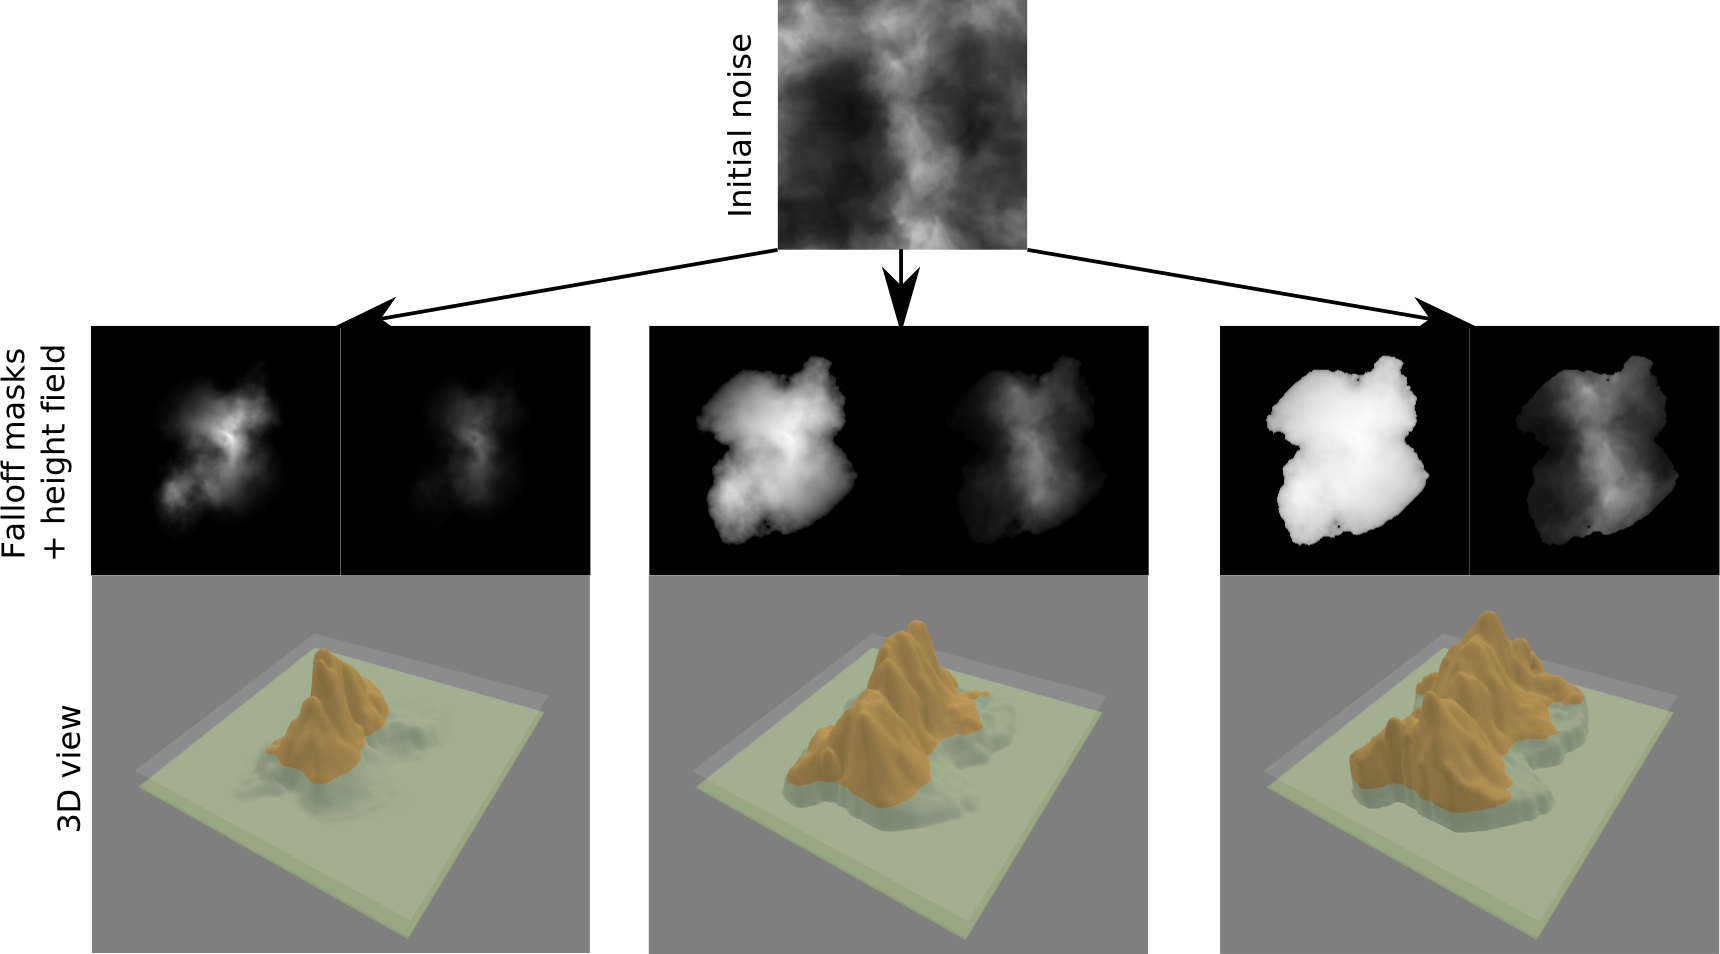
\includegraphics[width = \linewidth]{noise_examples3.pdf}
    \caption{Three different results of an island generated from noise functions. In each case, the initial height field is the same, computed through flow noise. The falloff masks are also generated with a combination of fBm noise mitigated by the euclidean distance from the image center, warp noise and gamma correction. The only parameter modified for each example is the gamma correction. The results are very different, and hardly controllable. It is also difficult to represent lagoons and reefs using this method.}
    \label{fig:coral-island_noise-example}
\end{figure}

Noise-based procedural generation remains one of the most widely used techniques for creating natural-looking terrains. Perlin noise \cite{Perlin1985}, Simplex noise \cite{Perlin2001}, and the Diamond-square algorithm \cite{Fournier1982} are foundational algorithms that generate pseudo-random yet continuous variations across a grid, producing terrain features that resemble organic landscapes. These techniques have been widely adopted in computer graphics and game development due to their efficiency and visual appeal.

Beyond basic noise functions, more advanced techniques such as fractal Brownian motion (fBm) and multifractal noise have been introduced to add finer-scale variation and detail \cite{Musgrave1989,Ebert2003}. FBm combines multiple layers, or "octaves," of noise at different frequencies and amplitudes, producing terrains that exhibit more realistic and varied features. The combination of noise with domain warping and signal processing techniques has been explored in depth in procedural modeling literature \cite{Reinhard2010}, enabling further control over visual complexity and terrain realism.

Noise functions are often paired with falloff maps to produce island-like terrains, where elevation gradually decreases toward the edges of the domain, mimicking coastlines and basic island shapes (see \cref{fig:coral-island_noise-example}). Various methods for enhancing island generation using noise and falloff blending have been proposed for applications in games and virtual worlds \cite{Olsen2004}. While these techniques excel at producing large, visually diverse landscapes quickly, they suffer from several key limitations when applied to the modeling of coral reef islands.

Critically, noise-based terrains lack grounding in geological or biological reality. They generate spatial patterns through mathematical noise, not through simulations of real-world processes such as volcanic subsidence or coral accretion. The signal processing parameters typically involved (frequency, lacunarity, gain, amplitude, ...) are tuned for visual effect rather than scientific plausibility. As highlighted in procedural modeling surveys \cite{Smelik2009,Galin2019}, this disconnect results in a lack of semantic control and poor correlation with actual environmental dynamics, making it difficult to represent phenomena like reef rings, lagoons, or atoll structures in a biologically or geologically coherent way.

Moreover, the biological aspects of coral growth are inherently tied to environmental conditions. Coral reefs form and persist only within specific ranges of water depth, sunlight, salinity, and water quality. Their growth patterns are further influenced by ecological health, nutrient availability, and symbiotic relationships. These dependencies are extremely difficult to capture in procedural noise systems, which are not designed to model such complex and coupled dynamics.

Our approach goes beyond the randomness of noise-based generation by incorporating real-world geological and biological processes into the terrain formation pipeline. Specifically, we model the gradual subsidence of volcanic islands and the upward growth of coral reefs, both of which are central to the long-term evolution of coral reef islands. By embedding these natural processes directly into the generation algorithm, we produce terrains that are not only more realistic but also more controllable. This integration of scientific modeling with procedural flexibility allows us to overcome the inherent limitations of traditional noise-based techniques and more accurately represent the complex formation of coral reef island systems.

\subsubsection{Simulation-based modeling}

Simulation-based terrain modeling methods aim to increase realism by replicating natural processes such as erosion, sediment transport, tectonic uplift, and vegetation growth. Unlike noise-based techniques, which rely on random functions, simulation-based approaches model causality and temporal dynamics to describe how a terrain evolves over time under physical or biological forces. These methods are often used to enhance base terrains, adding geologically plausible detail and structure \cite{Benes2006, Smelik2009}.

\subsubsubsection{Hydraulic and thermal erosion}

Hydraulic erosion models simulate the impact of flowing water on the landscape by modeling erosion, sediment pickup, transport, and deposition. Early implementations by Musgrave et al. \cite{Musgrave1989} laid the groundwork for erosion in procedural generation, while more recent works (e.g., \cite{Mei2007}) have accelerated these simulations using GPU architectures and particle-based methods. These simulations often follow Eulerian fluid models or Lagrangian particle systems to capture terrain displacement.

Thermal erosion, by contrast, simulates mass movement due to gravity, redistributing material from steeper slopes to gentler gradients, akin to landslides or soil creep \cite{Benes2006}. These erosion models generate realistic fluvial networks and landforms, but they are parameter-sensitive and computationally expensive.

Moreover, such models are generally designed for terrestrial landscapes and lack mechanisms for simulating underwater sedimentation, reef growth, or biogenic processes crucial to coral island formation. These models typically simulate time scales relevant to geomorphological processes (hundreds to thousands of years), which are mismatched with both the faster dynamics of biological processes like coral health and the slower geological evolution of reef islands.

\subsubsubsection{Tectonic uplift and geologic simulation}

Geological simulation approaches such as those proposed by Cordonnier et al. \cite{Cordonnier2016, Cordonnier2017a} and extended by Schott et al. \cite{Schott2023} model terrain evolution through crustal deformation and tectonic uplift. These methods simulate isostatic adjustments, plate tectonics, or local uplift phenomena, often over geological timescales.

Although well-suited for mountain-building processes or fault line modeling, these methods are not designed to account for biogenic terrain formation, such as coral reef accretion, which is critical for simulating coral reef islands. As a result, despite being physically grounded models, they do not capture the coupled geological and biological dynamics necessary for representing the long-term evolution of reef islands.

\subsubsubsection{Vegetation and ecosystem dynamics}

Some simulation-based terrain models integrate ecological dynamics to reflect the feedback between terrain and living systems. For instance, Ecormier-Nocca et al. \cite{Ecormier-Nocca2021} and Cordonnier et al. \cite{Cordonnier2017b} simulate interactions between vegetation and terrain erosion, modeling plant colonization, growth, and their influence on soil stability and moisture retention.

These ecosystem simulations allow more complex landscape evolution by considering biotic agents; however, they are designed primarily for terrestrial plants and temperate ecosystems. Coral colonies, in contrast, are marine organisms with strict environmental requirements such as limited depth, adequate sunlight, warm water temperatures, and clear water for photosynthesis via symbiotic algae. Accurately simulating these dependencies would require significant computation resources.

Furthermore, coral growth is not a passive process like sediment accumulation or root expansion, but an active accretion system that builds calcium carbonate structures over thousands of years. These unique growth mechanisms, constrained by marine ecology, fall outside the scope of existing vegetation or soil-plant-water feedback models.

\midConclusion

While simulation-based models represent a significant advancement over purely procedural approaches, they fall short in capturing the coupled geological and biological dynamics that shape coral reef islands. They are either computationally intensive, domain-specific, or biologically inapplicable, highlighting the need for a new class of terrain generation tools that embed long-term marine biogeomorphological processes into the procedural pipeline.




% \comment{Here, present hydraulic erosion (which will be developed indepth in \cref{chap:erosion}), then uplift simulation \cite{Cordonnier2017a,Cordonnier2016} and \cite{Schott2023}, then \cite{Ecormier-Nocca2021} and \cite{Cordonnier2017b} for simulating erosion + vegetation, but coral does not behave like a vegetal, nor fauna, nor geology. }



\subsection{Sketch-based terrain modeling}
\label{sec:coral-island_sota-sketches}

The term sketching encompasses several meanings: it can refer to performing gestures with the hand or body, creating a rough drawing, or outlining an idea in a simplified form. Accordingly, sketch-based modeling in 3D computer graphics can be understood through three complementary perspectives, each centered around a distinct core concept.

First, sketching may focus on interaction, where gestures captured through hand or body motion are used to manipulate virtual objects, often in immersive environments like virtual or augmented reality, drawing on established techniques such as sculpting and distortion \cite{Olsen2009, Cook2009}. Second, it can involve construction, where simple geometric primitives (curves, parametric shapes, implicit surfaces, ...) are combined under constraints to build more complex models. Finally, sketching may center on interpretation, where the user draws strokes on a 2D canvas and the system analyzes their meaning to generate a plausible 3D model.

While sketch-based modeling encompasses a wide range of techniques, including gesture-driven interaction in immersive environments, this work focuses primarily on the construction and interpretation aspects. In particular, construction serves as the foundation for procedural generation techniques using geometric primitives and constraints (addressed in this section), while interpretation becomes relevant when exploring data-driven approaches using deep learning to infer terrain structure from sketches (discussed in the following section). Interaction-based techniques, though significant in other contexts, fall outside the scope of this work. 

To distinguish clearly between the different aspects addressed in this chapter, we will refer to the constructive approach as sketch-based, and to the interpretive, learning-driven approach as learning-based. It is important to note, however, that the boundaries between these categories are inherently blurry and often overlap in practice.

In procedural terrain generation, sketch-based construction approaches enable users to shape landscapes by manipulating high-level geometric primitives through intuitive sketching interfaces. These methods allow the definition of key terrain features, such as mountains, valleys, and coastlines, by drawing their outlines on a two-dimensional canvas, which are then procedurally transformed into 2.5D or 3D terrain representations. This approach offers a high degree of artistic control, making it particularly effective for creative applications like video games and simulations, where modeling is primarily user-driven.

\subsubsection{Curve-based modeling}

Sketch-based terrain generation often begins with user-defined curves that act as high-level constraints to guide the shape of the terrain. These curves may represent silhouettes, ridgelines, valleys, or feature outlines. Once defined, they are interpreted by the system and translated into elevation changes through various computational techniques. This approach allows for intuitive control over large-scale landforms while maintaining a procedural foundation for terrain synthesis.

\AltTextImage{
    One of the earliest and most influential works in this domain is the system introduced by \citep{Gain2009}, which enables users to sketch silhouettes, ridges, and spine curves to define complex terrain structures. The method employs multiresolution surface deformation and propagates wavelet-based noise from the sketched features to their surroundings, allowing users to generate detailed, natural-looking terrains from minimal input. This approach demonstrated the effectiveness of combining intuitive sketch input with procedural detail synthesis.
    We draw direct inspiration from this work's dual-view sketching strategy, combining top-view and profile sketches, which closely aligns with our concentric curve and height-profile input approach.

    Expanding on this idea, \citep{Hnaidi2010} proposed a technique based on diffusion equations. In their method, curves are annotated with geometric constraints such as elevation or slope, and a diffusion process is used to interpolate these constraints across the terrain surface. This results in smooth, continuous elevation fields that conform to user-defined features such as rivers, ridgelines, or cliffs. The use of parameterized curves as terrain anchors allows for precise control over landform shaping, while maintaining a high degree of automation.
}{sketchingGain2009-vertical.png}{caption}{label}

\AltTextImage{
    In a different interaction paradigm, \citep{Tasse2014} introduced a first-person sketching interface, where users draw terrain silhouettes from a particular camera viewpoint. These silhouettes are then projected into 3D, and a deformation algorithm adjusts the terrain so that the drawn features are visible exactly as intended from the user's perspective. This method supports complex silhouettes with occlusions, T-junctions, and cusps, and represents a more immersive and perceptually grounded approach to sketch-based terrain editing.
}{sketchingTasse2014-vertical.png}{caption}{label}

These methods demonstrate the expressive power of curves as terrain-defining elements. By enabling users to sketch intuitive shapes and constraints, they bridge the gap between artistic intent and procedural complexity. Curve-driven approaches remain foundational in terrain modeling, particularly when user control over large-scale structure is essential. While we do not use the diffusion model, the idea of sketch-defined elevation constraints along curves informs our use of user-defined shape boundaries.


\subsubsection{Constraint-based modeling}

While curve-driven techniques provide intuitive shape design, constraint-based and gradient-based approaches focus on exerting precise control over terrain features through formal specifications such as elevation values, slopes, or gradient fields. These methods prioritize structural accuracy and procedural consistency, making them particularly suited to applications that demand terrain realism, integration with geographic data, or fine-grained editing capabilities.

\AltTextImage{
    A representative example of constraint-based modeling is presented by \citep{Gasch2020}, who propose a method for procedural terrain generation that respects user-defined elevation constraints. Their system allows users to fix values at specific control points (e.g., paths, landmarks) and then employs a system of equations to propagate these constraints throughout the terrain. Crucially, the method integrates these constraints with a noise-based procedural function to preserve natural randomness while conforming to user intent. This approach is especially valuable when generating terrains that must align with real-world data or gameplay constraints. 
    We do not adopt their constraint-solving mechanism, but conceptually relate our profile sketch input to a localized height constraint.
}{sketching-Gasch2020.png}{caption}{label}

\AltTextImage{
    Extending the idea of constrained procedural generation, \citep{Talgorn2018} introduce a real-time sketch-based terrain generation system based on a GPU-accelerated implementation of midpoint displacement. Users sketch curves with explicit elevation values, which act as absolute constraints, while the system extrapolates and interpolates terrain surfaces in real-time. Crucially, their model supports both global and local control over interpolation curvature and roughness, and introduces semantic labeling of sketched features (e.g., ridges vs. rivers) to influence how terrain propagates around constraints. This combination of sketch-based input, constraint propagation, and semantic control enables expressive, large-scale terrain modeling at interactive speeds. We do not reuse their fractal interpolation model, but we incorporate their notion of semantic labels and hierarchical constraint propagation to support real-time terrain shaping with sketch-defined features.
}{sketching-Talgorn2018.png}{caption}{label}

\AltTextImage{
    Building on the need for more intuitive editing, \citep{Guerin2022} introduce a novel paradigm by modeling terrain in the gradient domain. Rather than specifying elevation values directly, users interact with slope-based representations, allowing for the manipulation of terrain inclination and the integration of local edits into global terrain structure. By controlling terrain gradients and reconstructing elevation through integration, this method enables seamless blending between regions and supports a more natural editing workflow, particularly for sculpting realistic mountain ridges, valleys, or plateaus. 
    This gradient-domain editing approach offers interesting insights, but is not directly used, as we operate in the elevation domain with semantic control.
}{sketching-Guerin2022-vertical.png}{caption}{label}

Both approaches offer complementary strengths: constraint-based methods ensure precise adherence to user-defined features or data sources, while gradient-based systems provide fluid, perceptual control over terrain shaping. Together, they represent a shift toward high-level modeling tools that maintain procedural expressiveness while granting users a deeper degree of terrain control.

\subsubsection{Semantic terrain representation}
Beyond geometric sketching and low-level constraints, a third class of methods explores high-level terrain construction, where users guide terrain generation using abstract or semantic inputs. These approaches aim to simplify the authoring process by allowing users to describe what a terrain should contain (e.g., a mountain or a valley) without specifying how to generate it geometrically. Such methods often rely on symbolic sketching, sparse representations, or domain-specific visual cues, offering powerful tools for conceptual design and inverse procedural modeling.

\AltTextImage{
    In this vein, \citep{Genevaux2015} propose a method for representing terrains as sparse combinations of procedural primitives, referred to as "terrain atoms." These atoms are stored in a dictionary and can be either extracted from real-world data or generated synthetically. The terrain is modeled as a linear combination of these features, forming a Sparse Construction Tree that blends primitives in a compact and expressive form. This representation facilitates terrain editing, amplification, and reconstruction from coarse user input, making it ideal for scenarios that require terrain matching or abstract design control.
    While this work introduces a symbolic representation of terrain via atoms, it is not reused in our method, which instead relies on semantic label maps. 
}{sketching-Genevaux2015-1.png,sketching-Genevaux2015-2.png}{caption}{label}

\AltTextImage{
    A more illustrative and domain-specific use case is presented by \citep{Natali2012}, who introduce a system for rapid visualization of geological concepts. Here, users sketch schematic representations of subsurface structures such as faults, folds, or strata, and the system generates plausible 3D visualizations of geological terrains. The tool is designed primarily for educational and exploratory purposes, enabling geoscientists and students to create, manipulate, and communicate complex geological scenarios through intuitive sketch input. Although it extends beyond traditional terrain elevation modeling, the work exemplifies how sketch-based systems can operate on a conceptual level and support domain-specific semantics.
    This work inspired our use of sketch strokes to define deformation fields, although our implementation targets structured terrain generation rather than schematic visualization.
}{sketching-Natali-2012.png}{caption}{label}

These high-level approaches demonstrate the potential of sketch-based modeling not just as a geometric tool, but as a semantic interface between human intention and terrain synthesis. By abstracting terrain construction into symbolic or feature-based representations, they allow users to create rich, expressive landscapes without directly engaging with low-level geometry, making them particularly valuable for tasks involving conceptual design, education, and inverse procedural modeling.

\midConclusion

The works presented in this section illustrate the diversity of sketch-based approaches for constructive terrain modeling, from curve-driven shape control to constraint-based editing and semantic abstractions. While these methods offer valuable tools for intuitive user interaction and procedural shaping, they often lack ecological grounding, multi-view integration, or the ability to produce structured data suitable for training generative models. In our work, we reinterpret and adapt elements from these approaches such as dual-view sketching, curve-based region definition, and deformation fields, to support the generation of coral reef islands through a hybrid procedural and learning-based pipeline. This constructive sketch-based foundation enables us to balance user control with scalable terrain generation in data-sparse domains.

\comment{Also need to include \citep{Ketabchi2016}}

% \AltTextImage{


%     Sketching has been extended to geological modeling \cite{Patel2021}. \cite{Natali2012} proposed a system where users can interactively model underground layers by sketching subsurface structures. This provides a powerful tool for geologists and designers who need to model complex, multi-layered terrains, offering more control over both the surface and the subsurface.

%     The strokes added by the user are used to create a displacement field, deforming the vertices or the textures of the model. 

%     In our application we borrow this idea by generating a wind-field thanks to user strokes on a 2D canvas. This deformation field 
% }{sketching-Natali-2012.png}{Bla}{fig:sketching-natali-2012}

% \comment{
%     The next works uses diffusion equations to edit the landscapes in a natural manner.
% }
% \AltTextImage{
%     Sketch-based systems offer great flexibility, allowing users to directly define specific elements of the landscape according to their needs or preferences. For instance, \citep{Gain2009} introduced a multi-perspective sketching system that allows users to generate detailed landscapes by sketching from different angles. This method provides more control over the terrain's shape than traditional noise-based generation methods.
% }{sketchingGain2009-vertical-s.png}{From \cite{Gain2009}, a mountain is generated by a top-view shape and a height function}{fig:sketching-gain-2009}

% \AltTextImage{
%     Similarly, \citep{Tasse2014} explored sketching from the player's viewpoint, allowing users to dynamically define height information from within the virtual environment, creating an interactive terrain design experience.

%     The same is true for \cite{Hnaidi2010}.
% }{sketchingTasse2014-vertical-s.png}{From \cite{Tasse2014}, the first person view constraint allows for a sketching of mountains by a single stroke.}{fig:sketching-tasse-2014}

% \AltTextImage{
%     Curves are powerful geometrical tools as they are unaffected by the resolution of the terrain and only affected by the number of control points used to define them. Moreover, different works have been adding constraints on the curves drawn on the terrain, such as forcing all points at the position of a curve to be at a certain height, or that each side of the curve follow a certain gradient (see \cref{fig:sketching-guerin-2022}). In \cite{Guerin2022}, the authors applied diffusion on these constraints in order to propagate them smoothly and seamlessly around the sketch. Diffusion curves uses the heat diffusion equations to find an equilibrum \cite{Orzan2008}, which can be solved using multiresolution integrated in the GPU pipeline.
% }{sketching-Guerin2022.png}{From \cite{Guerin2022}, constraints are added to the surface of the terrain, including gradient constraint and height constraints, which are then diffused on the surface, allowing for the modeling of multiple landscape features}{fig:sketching-guerin-2022}


% In our work, we leverage the flexibility of sketching to define the key features of coral reef islands, such as the island shape, lagoons, and coral reefs, in a vectorized format. This is particularly important for modeling underwater and island landscapes, where these features are not simply surface elements but part of an evolving geological structure. By using sketches, we retain the semantic information of where the island and coral regions are located, which allows us to later apply our simplified model of Darwin's subsidence theory.

% % \wrapFigL{sketchingTalgorn2018.png}{0.25}{fig:sketching-taglorn-2018}{From \cite{Talgorn2018}, a mountain is generated by a top-view shape and a height function [Need to change the image to vertical]}

% Rather than focusing on detailed long-term or short-term evolution, our method adapts sketching to the unique requirements of island and underwater landscapes. Once the user defines the terrain layout through sketching, we apply a simplified subsidence model, where the volcanic island gradually sinks and coral reefs grow in response, remaining close to the water surface. This process provides a framework for simulating the evolution of the landscape in a geologically plausible manner.

% The key advantage of sketching in our system is that it combines the artistic control provided by traditional sketching methods with the ability to handle the geological processes specific to coral reef islands. By preserving the vectorized information from the sketch, we can accurately place and evolve features like lagoons and coral reefs, ensuring that the resulting terrain reflects both the user's design intent and the geological dynamics at play.




\subsection{Deep learning}
\label{sec:coral-island_sota-deep-learning}

\begin{figure}[H]
	\centering
	\includegraphics{schemaGAN_cGAN.jpg}
    \caption{The general structure of GAN and cGAN networks are similar: a generator network $G$ is trained to take some noise $z$ as input to try to create a "realistic" output $X_{\text{fake}}$ and a discriminator network $D$ is trained parallelly to distinguish generated data from real data. cGAN networks introduce an information of class $c$ in the input, which is used by the generator and discriminator in their inference process. In the end, only the generator is used to create new data. }
    \label{fig:coral-island_GAN-scheme}
\end{figure}

Over the past decade, deep learning has revolutionized many areas of computer graphics and procedural content creation by learning complex, data-driven priors directly from examples. Unlike purely procedural or sketch-based methods, which rely on hand-tuned noise functions or geometric constraints, neural networks can capture subtle patterns and high-frequency details without explicit programming of each effect. In terrain synthesis, this enables models to infer realistic elevation structures, textures, and region transitions from training data, even when that data is sparse or synthetic. In the context of coral-reef islands where high-resolution digital elevation models are rare, deep learning offers a way to abstract away low-level procedural rules and directly learn the mapping from semantic layouts (label maps) to plausible height fields. In the following sections, we first review general generative adversarial networks (GANs) and then focus on their conditional variant (cGAN), which forms the backbone of our sketch-to-terrain translation pipeline.

\subsubsection{Generative Aversarial Networks}
\label{sec:coral-island_sota-GAN}

Generative Adversarial Networks (GANs), introduced by \cite{Goodfellow2014}, are a class of generative models in which two neural networks are trained in opposition: a generator $G$ learns to produce synthetic data samples that resemble those from a target distribution, while a discriminator $D$ learns to distinguish real samples from those generated. Through this adversarial process, the generator improves its ability to mimic the underlying data distribution, enabling the creation of realistic outputs from random input.

GANs have been widely adopted for image synthesis, texture generation, and data augmentation, among other tasks. In terrain modeling, they offer the potential to generate plausible landforms by learning directly from real-world data, without requiring hand-crafted procedural rules. The following works demonstrate how different GAN variants have been applied to terrain synthesis, each with its own assumptions, design trade-offs, and limitations.



Early applications of GANs to terrain focused on unconditional generation, where elevation maps are synthesized from pure latent noise, without any spatial or semantic guidance. \citep{WulffJensen2018} trained a deep convolutional GAN (DCGAN) to produce realistic digital elevation models of mountainous landscapes, showing that terrain-like structures could emerge from purely data-driven learning. The model captured local elevation statistics and allowed for latent space interpolation, enabling smooth variations across generated terrains. However, the lack of spatial conditioning made it difficult to control or constrain specific features such as ridges, valleys, and coastlines, resulting in landscapes that reflected training set distributions but offered no means for intentional design.

\citep{Spick2019} extended this approach by introducing a Spatial GAN that generates height and texture maps jointly. By conditioning the generation process on spatial coordinates, their model enforced local consistency and reduced structural artifacts. This integration simplified the content pipeline by fusing geometry and appearance into a single pass. Yet despite improved quality, the generation process remained fundamentally uncontrolled: there was no way for users to specify terrain layout, features, or semantics. As with earlier GANs, the model learned to mimic terrain distributions but could not support authoring or guided synthesis.

To address the lack of control inherent in purely noise-driven GANs, later works introduced multi-stage architectures in which a second, conditional GAN refines or interprets the output of a first-stage generator. \citep{Beckham2017} proposed a two-step pipeline where a DCGAN generates bare terrain heightmaps from noise, and a conditional pix2pix network adds texture based on semantic cues. This separation of geometry and appearance allows for basic stylization and terrain remixing, but still suffers from the lack of control in the initial heightmap generation. In a conceptually similar structure, \citep{Panagiotou2020} reversed the mapping: an unconditional GAN first synthesizes aerial RGB imagery from noise, which is then passed to a cGAN trained to predict plausible DEMs. While this image-to-DEM translation enables realistic terrain reconstruction, it depends on large collections of paired data and lacks any semantic or structural control from the user. In both cases, despite the introduction of a conditional refinement stage, the generation process remains fundamentally anchored in an unconstrained latent input, offering limited authoring capability and no principled way to shape landform structures.

These approaches show a shift toward using conditional models to guide terrain generation with more structure. But because they still start from random noise, they offer little real control over the layout or meaning of the terrain. A natural next step is to guide the generation process directly from user-defined semantic inputs, such as sketches or label maps, to produce terrain that reflects both the training data and the user's intent.


\subsubsection{Conditional GANs for terrain generation}
\label{sec:coral-island_sota-cGAN}

While traditional GANs generate data from noise, Conditional GANs (cGANs) extend this concept by incorporating side information, often called class map or label map, to guide generation toward user-specified outcomes \cite{Mirza2014}. This makes them particularly attractive for structured content synthesis tasks, including terrain generation, where user input often defines large-scale layout while realism must emerge from learned detail. The pix2pix framework by \citep{Isola2017} is the canonical cGAN formulation for image-to-image translation. It uses a U-Net generator conditioned on an input image (a sketch or a label map, for example), and a PatchGAN discriminator that evaluates realism at the patch level, encouraging fine detail and local consistency.

\begin{figure}[H]
\centering
\includegraphics[width = 0.8 \linewidth]{example_pix2pix_facade.png}
\includegraphics[width = 0.8 \linewidth]{example_pix2pix_maps.png}
\caption{Example of pix2pix image-to-image translation: (top) a trained model converts semantic label maps into realistic façade images, or (bottom) the construction of highly plausible aerial images from navigation map sketches. This paradigm generalizes to many tasks, including terrain generation.}
\label{fig:coral-island_pix2pix-example}
\end{figure}

In the domain of terrain generation, the use of cGANs remains surprisingly rare. The most directly relevant precedent is the work of \citep{Guerin2017}, who train a pix2pix-style cGAN to map sketched terrain features such as valleys, ridgelines, or peaks, into full-resolution digital elevation models (DEMs). Their results demonstrate that cGANs can plausibly reconstruct complex topographic forms from sparse semantic cues, offering a promising balance between user control and learned realism. Similarly, \citep{Sisodia2022} applies a cGAN to generate stylized terrain heightmaps from sketch maps in the context of 2D game environments, further validating the sketch-to-terrain pipeline.

Another related line of work explores learning-based terrain synthesis using partial or sparse spatial inputs. \citep{Voulgaris2021} propose a GAN-based system that maps sparse "altitude dot" maps to plausible terrain imagery, acting as a minimal-interaction generative authoring tool. While not strictly a cGAN, their system reflects a similar spirit: conditioning generation on lightweight user constraints. Likewise, \cite{Panagiotou2020} and \cite{Beckham2017} trained a cGAN to invert RGB satellite imagery into elevation data, framing terrain modeling as an appearance-to-geometry and geometry-to-appearance translation task. However, such image-to-DEM (and DEM-to-image) systems are heavily dependent on large paired datasets, which limits their applicability in settings like coral reef islands, where training data are scarce.

Despite this emerging body of work, there is still no standard pipeline for generating detailed terrains from semantic layout maps using cGANs, particularly in biologically driven environments like coral reef islands. This gap is outstanding given the success of cGANs in analogous image synthesis domains, and the explosive progress in the field of deep generative models. The potential of this approach remains underexploited, especially when it comes to coupling user control with long-term geological plausibility.

\midConclusion

In our method, we address this gap by training a pix2pix cGAN to transform label maps (semantic region maps produced by procedural sketch-based modeling) into realistic coral reef island height fields. Each input map encodes key zones of an island (e.g., lagoon, reef crest, beach, island core) using categorical labels, serving as a semantic constraints for terrain synthesis. The cGAN generator learns to condition elevation details on both the global layout and the implicit patterns encoded in the training data. By generating our own synthetic dataset with procedurally modeled coral islands (see \cref{fig:coral-island_difficulties-dataset}), we overcome the shortage of labeled elevation data and enforce geological coherence via data generation design.

\begin{figure}[H]
\includegraphics[width=0.9 \linewidth]{placeholder.pdf}
\caption{Examples of procedural region maps used for training: left to right, canonical island, off-center island, elongated shapes, and multi-island scenes. These maps serve as semantic inputs to the cGAN.}
\label{fig:coral-island_difficulties-dataset}
\end{figure}

This setup offers several key advantages: it respects user-defined structure while allowing the generator to introduce realistic variation, it removes procedural biases such as radial symmetry and fixed island typologies, and it enables the generation of irregular, non-circular landforms while implicitly modeling geological processes like subsidence and coral accretion through training-time priors. 

In this context, conditional GANs emerge as a powerful yet underutilized tool for terrain modeling. By training on procedurally generated coral island data, we show that sketch-conditioned learning can effectively bridge the gap between high-level user intent and geologically plausible terrain synthesis.





% To steer generation toward a desired output, Conditional GANs (cGANs) augment both $G$ and $D$ with side information $y$, such as class labels or input images \cite{Mirza2014}.  The objective becomes
% \[
% \min_G \max_D \; \mathbb{E}_{x,y\sim p_{\text{data}}}[\log D(x,y)] \;+\;
% \mathbb{E}_{z\sim p_z,y\sim p_{\text{data}}}[\log(1 - D(G(z,y),y))].
% \]
% The pix2pix model, proposed in \cite{Isola2017}, applied a U-Net generator and PatchGAN discriminator to learn mappings between paired images such as edge maps to photographs, label maps to facades, and more, demonstrating sharp, structurally coherent translations on a variety of vision tasks.  The key insight is that $y$ can encode spatial layouts (semantic labels, sketches) that $G$ uses to condition high-frequency detail synthesis, while $D$ focuses on local realism through a patchwise adversarial loss.

% \begin{figure}[H]
% 	\centering
% 	\includegraphics[width = 0.8 \linewidth]{example_pix2pix_facade.png}
%     \caption{Example of application of the pix2pix deep learning model: From a trained dataset of facades composed of real world images associated with their label maps, providing a new label map outputs a realistic facade image. }
%     \label{fig:coral-island_pix2pix-example}
% \end{figure}


% \comment{
%     \cite{Isola2017} demonstrated pix2pix on tasks like maps-to-aerial photos, which inspires our use of it for sketch-to-terrain translation.
% }

% \comment{Talk about \cite{Voulgaris2021} (sparse height points in a 2D space to generate plausible aerial images (no geometry)).}

% \AltTextImage{
%     In terrain generation, or more specifically terrain authoring, cGANs have been applied to generate diverse landscapes by learning the patterns and features found in real-world terrains. For example, \citep{Guerin2017} demonstrated how cGANs can be used to transform 2D sketches into 3D terrains by training the network on a dataset of terrain features, allowing the system to generate new landscapes based on simple user input (see \cref{fig:coral-island_Guerin2017-example}). cGANs are particularly well-suited for this task because they can capture the subtle details of terrain that would be difficult to model explicitly, such as the natural flow of elevation or the transitions between different terrain types.
% }{Guerin_example_cgan.png}{\cite{Guerin2017} trains a cGAN from real world data, such that a sketch drawn by the user gets transformed into a plausible height field respecting the user constraints.}{fig:coral-island_Guerin2017-example}

% In the case of terrain generation, a cGAN allows the user to specify high-level constraints (such as the regions where different terrain types should be) while the generator fills in the finer details based on what it has learned from the training data. This makes cGANs particularly effective in applications where a mix of user input and data-driven generation is required, as the user can control the broad layout of the terrain while the model ensures that the resulting terrain looks natural and plausible.

% In our approach, we use a cGAN to generate coral reef islands, providing a balance between user control and realistic terrain generation. After the initial algorithm outlines the regions of the island such as the island itself, beaches, and lagoons, these regions are transformed into a single image, where each pixel represents a different region ID. This image is used as the input for the cGAN, which conditions the generation process on this initial layout.


% The cGAN is trained on a dataset of island examples, which are created by our own procedural generation algorithm and further augmented to introduce a wide variety of shapes and features. This training allows the cGAN to generate coral reef islands that follow the high-level layout provided by the user while introducing natural variations and details that reflect real-world island characteristics. By conditioning the cGAN on the user-defined region map, we ensure that the generated islands maintain structural coherence while still exhibiting realistic features like smooth transitions between regions, varied terrain, and non-circular shapes.

% One of the key advantages of using a cGAN in our system is its ability to overcome procedural constraints. Traditional procedural generation methods often impose limitations like radial symmetry or require islands to follow overly simplified geometries. With the cGAN, these constraints can be lifted. The model can generate irregular, non-circular islands that adhere to the user's input but introduce a level of complexity and realism that would be difficult to achieve with purely procedural methods.

% \begin{figure}[H]
%     \includegraphics[width=0.9 \linewidth]{placeholder.pdf}
%     \caption{Additional difficulties are added to our dataset: from left to right, a simple map, translation from the center, non-radial map, multiple islands}
%     \label{fig:coral-island_difficulties-dataset}
% \end{figure}

% Additionally, the cGAN ensures that the generated island terrain aligns with the geological processes modeled in the system, such as subsidence and coral reef growth. By training the cGAN on thousands of examples that reflect these processes, we ensure that the final generated island models are both flexible and geologically plausible. The combination of user-driven design and data-driven generation through the cGAN allows for the creation of coral reef islands that are not only tailored to the user's input but also realistic in their form and structure.

% \midConclusion
% In summary, traditional procedural methods can create terrains but struggle with fine realism and user-directed specific shapes, sketch-based methods allow control but typically lack automated detail refinement, and GAN-based generation can produce realistic outputs but is constrained by data availability. Our approach addresses these gaps by combining a user-friendly sketch interface with a cGAN trained on procedurally generated examples, effectively merging the strengths of procedural and learned methods.



% \comment{
%     Early work by \cite{Goodfellow2014} introduced GANs ...  %, which have since been applied to terrain: e.g., researchers trained GANs on satellite elevation data to produce realistic mountains. Others have explored GANs for game level generation, showing neural nets can capture design patterns. However, these all rely on large training datasets of real examples, a luxury we don't have for coral reef islands.
% }

% A Generative Adversarial Network (GAN) consists of two competing neural networks: a generator that attempts to produce realistic data, and a discriminator that tries to distinguish between real and generated data. In the conditional GAN (cGAN) variant, both the generator and discriminator are conditioned on some input, meaning the generated output is influenced by additional information, such as a label map or image.



% The training dynamics of Generative Adversarial Networks (GANs) poses the challenge of simultaneously training two interconnected networks: the generator and the discriminator. The discriminator's accuracy crucially influences the generator's training outcomes. A discriminator that fails to accurately classify real from generated data may provide misleading feedback to the generator, hindering its ability to learn and improve. Conversely, an overly competent discriminator can excessively penalize the generator, stifling any potential for it to refine its outputs. This can result in the generator settling for a suboptimal minima, where it continuously generates non-diverse or overly simplistic outputs.

% Achieving an optimal balance between the performance of the generator and the discriminator involves meticulous tuning of hyperparameters. This balance is critical because it avoids the well-documented problem of mode collapse, where the generator learns to produce a limited variety of outputs [SOURCES]. It also ensures that the generator has enough leeway to explore the data distribution effectively without being overly constrained by the discriminator.

% Strategies such as employing adaptive learning rates for the discriminator or using different training frequencies for each network can help mitigate these issues. For example, researchers have found that updating the generator less frequently than the discriminator can prevent the discriminator from becoming too strong too quickly, thus supporting a more balanced training process. [SOURCES]

% Other approaches like curriculum learning can further optimize the training process. Curriculum learning strategically increases the complexity of training data over time, gradually challenging the model to improve its capabilities without overwhelming it initially. This method is particularly effective in preventing common pitfalls such as mode collapse by ensuring that the generator learns to replicate an increasingly diverse set of outputs. [SOURCES]


% \comment{Quickly present \cite{WulffJensen2018} (DC GAN), \cite{Spick2019} (SGAN, which is almost exactly the same thing, but generates height+texture in one pass), \cite{Beckham2017} (height field generated from random, allowing interpolation, and texture added by cGAN), \cite{Panagiotou2020} (exactly the other direction than Beckham), all are trained from real images}

% \subsubsection{Conditional Generative Adversarial Networks}
% \label{sec:coral-island_sota-cGAN}

% For island generation, we use the pix2pix model, a specific cGAN designed for image-to-image translation. In this case, the input to the generator is a label map which is a 2D image where each pixel is assigned an ID representing a different region of the island (e.g., island body, beach, lagoon, coral reef). The output is an image where each pixel corresponds to the elevation of the terrain at that point, ie. a height field.


% \begin{figure}[H]
% 	\centering
% 	\includegraphics[width = 0.8 \linewidth]{example_pix2pix_facade.png}
%     \caption{Example of application of the pix2pix deep learning model: From a trained dataset of facades composed of real world images associated with their label maps, providing a new label map outputs a realistic facade image. }
%     \label{fig:coral-island_pix2pix-example}
% \end{figure}


% \comment{
%     \cite{Isola2017} demonstrated pix2pix on tasks like maps-to-aerial photos, which inspires our use of it for sketch-to-terrain translation.
% }


% The pix2pix model operates on the framework of a conditional GAN, where the generator model is typically a U-Net-based architecture, and the discriminator is a PatchGAN. This structure allows the generator to produce full-resolution images while the discriminator focuses on classifying if individual sections of the image are real or fake. For island terrain generation, the U-Net architecture is particularly advantageous due to its ability to handle detailed spatial hierarchies, which is essential when translating simple label maps into complex height fields. 

% \comment{Talk about \cite{Sisodia2022} (Use of pix2pix for terrain gen + ESRGAN [superresolution model] for more details [papier a chier])}


% The cGAN model was chosen for this task because it allows us to overcome some of the constraints of the initial procedural algorithm. While the first algorithm generates island terrains based on radial symmetry and a limited set of input parameters, cGAN can generate more complex and varied terrains by learning from a large dataset of examples. Specifically, the use of cGAN addresses the following challenges:
% \begin{Itemize}
%     \Item{Increased variety:} The cGAN model can generate a wide range of island shapes and terrains by learning from the dataset. This allows for the creation of terrains that go beyond the predefined structures of the initial algorithm, introducing more natural variation in island features.

%     \Item{Overcoming constraints:} In the initial algorithm, islands are always centered in the image and adhere to a radial symmetry. Using cGAN, we apply data augmentation (translation, scaling, and copy-pasting multiple islands in one sample) to remove these constraints, allowing islands to take more irregular shapes and positions.

%     \Item{Flexibility:} Once trained, the cGAN model acts as a \remove{black box}{} that generates island terrains based on the label input. While this confronts the user to randomness during the generation process, the model can produce a variety of terrains that still respect the underlying structure of the label map. This enables a flexible, rapid generation process without requiring the user to fine-tune unintuitive parameters manually.
% \end{Itemize}

% The cGAN model is trained using a dataset of island terrains generated by the initial algorithm. To create this dataset, the algorithm randomly generates top-view shapes for the island's features, adds noise such as fractional Brownian motion, and introduces random wind velocity fields. The profile function remains consistent in determining the relative positions of the island, beach, and lagoon, but the top-view shapes vary through noise and deformation.


% However, given the specific requirements of our framework where ease of implementation is a priority, and the nature of the outputs (synthetic representations of island topographies) where visual appeal is more critical than precise accuracy, a different approach is justified. In this context, employing a pretrained model can significantly reduce the risk of training instabilities such as mode collapse while simplifying the development process. By using a pretrained model, we leverage previously learned features and patterns, which can facilitate a more stable and efficient training phase. As such, randomly shuffling the easy and difficult examples in the training schedule is sufficient to keep the model progressing.



% \subsubsection{Deep learning for terrain generation}
% \label{sec:coral-island_sota-cGAN-for-terrains}

% \begin{figure}[H]
%     \includegraphics[width=0.9 \linewidth]{Guerin_example_cgan.png}
%     \caption{\cite{Guerin2017} trains a cGAN from real world data, such that a sketch drawn by the user gets transformed into a plausible height field respecting the user constraints.}
%     \label{fig:coral-island_Guerin2017-example}
% \end{figure}

% \comment{Talk about \cite{Voulgaris2021} (sparse height points in a 2D space to generate plausible aerial images (no geometry)).}

% In terrain generation, GANs have been applied to generate diverse landscapes by learning the patterns and features found in real-world terrains. For example, \citep{Guerin2017} demonstrated how GANs can be used to transform 2D sketches into 3D terrains by training the network on a dataset of terrain features, allowing the system to generate new landscapes based on simple user input. GANs are particularly well-suited for this task because they can capture the subtle details of terrain that would be difficult to model explicitly, such as the natural flow of elevation or the transitions between different terrain types.

% A variant of GANs, known as Conditional Generative Adversarial Networks (cGANs), takes the power of GANs one step further by allowing the generated data to be conditioned on additional inputs. In a cGAN, both the generator and the discriminator receive additional information such as a class label, a sketch, or an image, that guides the generation process. This makes cGANs particularly useful for terrain generation tasks where users want to control specific aspects of the output while still relying on the model to generate realistic details.

% In the case of terrain generation, a cGAN allows the user to specify high-level constraints (such as the regions where different terrain types should be) while the generator fills in the finer details based on what it has learned from the training data. This makes cGANs particularly effective in applications where a mix of user input and data-driven generation is required, as the user can control the broad layout of the terrain while the model ensures that the resulting terrain looks natural and plausible.





\section{Description of our method}
\label{sec:coral-island_method-description}


\begin{figure}[H]
    \includegraphics[]{pipeline_full.pdf}
    \caption{Our method is split in three interleaved stages: the generation process (\cref{sec:coral-island_example-generation}) which creates pairs of height fields and label maps of an island from sketches, the model training (\cref{sec:coral-island_cGAN-training}) which use a synthetic dataset from the previous stage to obtain a cGAN model that generates height fields from label maps to remove the constraints embedded in the initial generation process, and finally, the inference process (\cref{sec:coral-island_results}) uses the trained cGAN to generate the final height fields, including the coral generation process, automatically. }
    \label{fig:coral-island_pipeline}
\end{figure}

Our method for generating coral reef islands combines user-driven sketching, procedural techniques, and deep learning to create realistic and varied island terrains (\cref{fig:coral-island_pipeline}). 

The pipeline consists of two distinct phases: a procedural data-generation phase and a deep-learning-driven inference phase. 

\subsection{Procedural generation phase}
\label{sec:coral-island_proc-phase}

In the initial procedural phase, the user sketches key island features from two complementary viewpoints: a top view, defining the horizontal layout of island features (island boundaries, beach width, lagoon areas, coral reefs), and a profile view, specifying the vertical elevation profile from island center to ocean (\cref{sec:coral-island_generation-initial}).

Additionally, users can sketch a wind deformation map, enabling simulation of natural erosion patterns caused by wind and waves (\cref{sec:coral-island_wind-deformation}).

From these sketches, the procedural system generates a synthetic island terrain with the keep-up stategy of coral reefs (\cref{sec:coral-island_coral-reef}) and a corresponding semantic label map, where each pixel indicates its region type (island, beach, lagoon, reef, abyss) (\cref{sec:coral-island_procedural-output}).




\subsubsection*{User interaction}
\label{sec:coral-island_description-UI}

\begin{figure}[H]
    \centering
    \includegraphics[width = 0.9 \linewidth]{user_interaction_generation.png}
    \caption{The user can interact directly on the island by editing the different canvases in no specific order. This UI shows, from left to right, the top-view sketch with the different outlines of each regions, the profile-view sketch with the outlines represented in dotted lines, the wind velocity sketch drawn with strokes (last stroke is visible), and the resistance function showing here a high resistance at the top of the island and on the front reef.}
    \label{fig:coral-island_wind-from-strokes-interaction}
\end{figure}

As users draw the top-view and profile-view sketches, the system provides real-time feedback on the resulting terrain. The top-view sketch influences the horizontal layout of the island, while the profile-view sketch defines its vertical structure. These sketches can be adjusted independently, allowing the user to fine-tune both the outline and elevation of the island.

While sketching the basic shape, users can apply wind deformation strokes to modify the island's features further. These strokes represent wind and wave influences, distorting the island's shape to introduce more natural, non-radial features such as indentations along the coastline, variable lagoon shapes, or concave formations. The system automatically applies these deformations, providing real-time feedback as the user interacts with the terrain.

This interactive process, combining sketches and wind deformation, allows users to quickly iterate on their designs, refining the terrain to meet specific aesthetic or functional goals.


\comment{Add output description from full procedural}

\subsection{Learning-based generation phase}
\label{sec:coral-island_cGAN-phase}

We repeat this procedural generation process many times with varied parameters (different shapes, scales, subsidence levels, and wind patterns) to create a large synthetic dataset (\cref{sec:coral-island_dataset-generation}). Each dataset entry consists of a label map paired with its procedurally generated terrain height field. Data augmentation is applied to the generated pairs to reduce the impact of the constraints induced from the procedural method (\cref{sec:coral-island_data-augmentation}).

We use this dataset to train a Conditional Generative Adversarial Network (cGAN), specifically the pix2pix architecture, capable of translating label semantic maps into realistic terrain height fields (\cref{sec:coral-island_cGAN-output}).

After training, the procedural step becomes unnecessary. To generate new island terrains, the user only needs to provide a label semantic map as input to the trained cGAN. The cGAN then synthesizes realistic island elevation details directly, capturing learned geological and geomorphological patterns from the synthetic training data (\cref{sec:coral-island_results}).

\subsubsection*{User interaction}
\label{sec:coral-island_cGAN-phase-interaction}

Thus, the trained cGAN provides a user-friendly interface: users draw or edit simple label maps (regions) to rapidly generate diverse, geologically plausible coral reef island terrains, incorporating realistic features such as smooth transitions between regions, detailed coral reef structures, and naturally varied shapes free from procedural constraints.

\midConclusion

This combined procedural-and-learning approach provides a simple, flexible, and powerful tool for island terrain generation, enabling users to intuitively generate realistic and diverse coral reef islands aligned with real-world geological and biological processes such as volcanic subsidence, coral reef growth, and wind-driven erosion.






















\section{Procedural island generation}
\label{sec:coral-island_example-generation}

\begin{figure}[H]
	\centering
	\autofitgraphics[]{placeholder.pdf}
    \caption{The example generation fully takes its potential in the procedural techniques, using sketches from the user (top-view sketch, profile-view sketch, wind sketch, and resistance sketch) to generate a height field in accordance with a label map. }
    \label{fig:coral-island_example-pipeline}
\end{figure}

The generation of coral reef island terrains involves a structured process that takes the user's sketches and produces a complete 3D terrain model. This process begins with the creation of the initial height field based on the user's input, followed by the application of wind deformation to introduce natural variations, and concludes with the integration of coral reef features through subsidence and coral growth modeling.





% \subsection{User inputs}
% \label{sec:coral-island_example-inputs}

The generation of coral reef islands in this system begins with two intuitive sketch-based inputs from the user: a top-view sketch and a profile-view sketch, which define the islands horizontal layout and vertical elevation profile. In addition to these sketches, the user can further refine the terrain by applying wind deformation strokes, which simulate the effects of wind and waves on the islands shape. This combination of sketches and wind inputs gives users precise control over both the islands structure and its natural variations, such as irregular coastlines or concave features. We will present the usefulness of these sketches in this section, and describe the technical details in the next section.

% \subsubsection{Top-view sketch}
% \label{sec:coral-island_top-view}
\subsection{Initial height field generation}
\label{sec:coral-island_generation-initial}


\begin{figure}[H]
	\centering
    \autofitgraphics[]{Cicia_island.png, Cicia_island-outlines.png}
	\includegraphics[width=0.90 \linewidth]{Cicia_island-3D.png}
    \caption{(Left) A real world example of aerial image (and 3D visualization on bottom) of an island (Cicia Island) may be segmented in regions. (Right) We can represent the different regions by the boundaries they form.}
    \label{fig:coral-island_top-view-sketch}
\end{figure}

The top-view sketch defines the islands outline as seen from above. Using a simple drawing interface, the user can delineate the boundaries between key regions of the island, including the island itself, the beaches, the lagoon, and the surrounding abyss. The system assumes that these regions are arranged concentrically around the center of the island, with each boundary defined by a radial distance from the center.

Each region's boundary is represented in polar coordinates, with $\radius_\p$ indicating the radial distance from the islands center and $\angl_\p$ representing the angular position. This polar representation allows the system to map the users sketch onto a circular framework, ensuring smooth transitions between regions and maintaining a coherent layout for the island.

In this sketch, the user defines the overall horizontal layout of the island, including the size and shape of each feature. Variations in the outline are introduced by allowing the radial distances to vary with angle, ensuring that the island is not strictly symmetrical and introducing more natural, irregular shapes.

\begin{figure}[H]
    \autofitgraphics[]{binary-heights-input-only-outlines-2.png, binary-heights-output-only-heightmap-2.png, binary-heights-render-2.png}
    \caption{Using only the outlines of the island as a input sketch, we can provide a height to each point of the field depending on the region in which it rely.}
    \label{fig:coral-island_procedural-height-only}
\end{figure}

% \subsubsection{Profile-view sketch}
% \label{sec:coral-island_profile-view}

\begin{figure}[H]
	\centering
    \autofitgraphics[]{profileFunction.pdf, schema_profile.jpg}
    \caption{(Left) A profile function $\heightProfile$ is defined as a 1D function and represents the surface from the center of the island to the abysses. (Right) The cross-section representation of an island is often represented as a 1D function defined using terrain features as landmarks. }
    \label{fig:coral-island_profile-function}
\end{figure}

The profile-view sketch defines the vertical elevation profile of the island along any radial direction, offering control over the islands height. In this view, the user specifies the elevation of different regions of the island, such as the island peak, beach, lagoon, abyss, and everything in-between, by drawing the corresponding profile curve.

The regions outlines correspond to key terrain transitions: the highest point of the island (center), the island border, the beach, the lagoon, and the deep-sea abyss. The system uses these milestones to interpolate a continuous 1D height function $\heightProfile(\distRegions)$, where $\distRegions$ represents a non-uniform region distance from the islands center, and $h = \heightProfile(\distRegions)$ gives the height at each point. This continuous profile ensures smooth elevation transitions across the island.

By combining the top-view and profile-view sketches, the system can generate a full 3D terrain model that accurately reflects the users design by revolution modeling.

The generation of the coral reef island terrain begins by transforming the user-defined top-view and profile-view sketches into a coherent 3D height field. This process combines the radial layout of the top-view sketch with the elevation information provided by the profile-view sketch, creating a terrain that accurately represents the desired features, such as the island, beaches, lagoons, and abyss.

For any point $\p$ on the terrain, the system first computes the polar coordinates $(\radius_\p, \angl_\p)$, where $\radius_\p$ is the radial distance from the island's center, and $\angl_\p$ is the angular component. The radial distance $\radius_\p$ is used to determine which region the point belongs to (island, beach, lagoon, reef, or abyss). The user-defined outlines in the profile sketch specify the radial limits between these regions.

\AltTextImage{
Each point's height is determined by the profile function $\heightProfile(\distRegions)$, where $\distRegions$ represents a "piecewise parametric distance" from the island's center. The piecewise parametric distance works by dividing the radial distance from the center into segments, defined by these region boundaries. Each segment corresponds to a distinct region of the terrain, and within each segment, the distance $\distRegions$ is interpolated between the region boundaries. For a point $\p$ lying between two boundaries $\Radius_{i}$ and $\Radius_{i+1}$, the distance $\distRegions_\p$ is calculated as:

\begin{align}
    \distRegions_\p = i + \frac{\radius_\p - \Radius_{i}}{\Radius_{i + 1} - \Radius_{i}}
\end{align}
where $i$ is the index of the nearest lower region boundary. This method allows for smooth transitions between regions, even when the spacing between boundaries varies. 

}{placeholder.pdf}{A drawing showing what $\tilde{x}$ represents on a top-view sketch}{fig:coral-island_parametric-distance}

For any point $\p$, the height is finally computed as:
\begin{align}
    h(\p) = \heightProfile(\distRegions_\p)
\end{align}

This approach ensures that the height field accurately follows the elevation profile specified by the user while maintaining smooth transitions between different regions of the island.

The result is a height field that captures both the radial structure of the island (from the top-view sketch) and the vertical elevation profile (from the profile-view sketch), producing a realistic representation of islands with smooth transitions between the key terrain features.

\begin{figure}[H]
    \autofitgraphics[]{smooth-input-outline-heights-1.png, smooth-output-heights-1.png, smooth-render-1.png}
    \autofitgraphics[]{smooth-input-outline-heights-2.png, smooth-output-heights-2.png, smooth-render-2.png}
    \autofitgraphics[]{smooth-input-outline-heights-3.png, smooth-output-heights-3.png, smooth-render-3.png}
    \caption{Providing a smooth function between each region results in islands with plausible reliefs. We fixed the outlines while editing only the height function in order to produce, from top to bottom, a low island, a coral reef island, and finally an identical island without the reef. }
    \label{fig:coral-island_procedural-smooth-heights}
\end{figure}





\subsubsection{Wind deformation}
\label{sec:coral-island_wind-deformation}
% \subsubsection{Wind velocity field}
% \label{sec:coral-island_wind-view}

\begin{figure}[H]
    \centering
    \includegraphics[width = 0.8 \linewidth]{windByStrokes.pdf}
    \caption{From the parametric curve defined by a user (red), we define the velocity field by considering the velocity (first derivative) of the curve at the closest point $\closestCp$, modulated by a gaussian distance function $G(x)$. }
    \label{fig:coral-island_wind-from-strokes}
\end{figure}

In addition to the sketches, the user can influence the shape of the island by defining a wind velocity field. This field simulates the effects of wind and wave erosion on the island's surface, introducing natural deformations such as coastline indentations, and more importantly allow the user to break the radial symmetry constraint.

The wind field is represented as a series of wind strokes drawn by the user on a 2D canvas. Each stroke represents a parametric curve, where the direction and strength of the wind are encoded as a vector field. The user controls the wind's direction by drawing these curves, and the system interprets the strokes to create a velocity field that defines how the terrain should be deformed.

As the user draws a wind stroke, the system generates a set of control points along the curve, with the option to adjust the stroke's width. The width of each stroke determines the area of influence around the curve, where wider strokes result in broader deformations of the terrain.
The deformation strength decreases with distance from the wind curve using a Gaussian falloff function using the stroke width as standard deviation, ensuring that the terrain transitions smoothly from deformed regions to non-deformed areas.
Once the wind strokes are applied, the system processes the wind velocity field by displacing the terrain points accordingly. The height field, originally generated from the user's sketches, is modified by the wind field to create non-radial features, breaking the initial radial symmetry and producing a more organic island shape.








% \subsection{Generation process}
% \label{sec:coral-island_generation-process}
% The generation of coral reef island terrains involves a structured process that takes the user's sketches and produces a complete 3D terrain model. This process begins with the creation of the initial height field based on the user's input, followed by the application of wind deformation to introduce natural variations, and concludes with the integration of coral reef features through subsidence and coral growth modeling.

% \subsubsection{Initial height field generation}
% \label{sec:coral-island_generation-initial}
% The generation of the coral reef island terrain begins by transforming the user-defined top-view and profile-view sketches into a coherent 3D height field. This process combines the radial layout of the top-view sketch with the elevation information provided by the profile-view sketch, creating a terrain that accurately represents the desired features, such as the island, beaches, lagoons, and abyss.

% For any point $\p$ on the terrain, the system first computes the polar coordinates $(\radius_\p, \angl_\p)$, where $\radius_\p$ is the radial distance from the island's center, and $\angl_\p$ is the angular component. The radial distance $\radius_\p$ is used to determine which region the point belongs to (island, beach, lagoon, reef, or abyss). The user-defined outlines in the profile sketch specify the radial limits between these regions.

% Each point's height is determined by the profile function $\heightProfile(\distRegions)$, where $\distRegions$ represents a "piecewise parametric distance" from the island's center. The piecewise parametric distance works by dividing the radial distance from the center into segments, defined by these region boundaries. Each segment corresponds to a distinct region of the terrain, and within each segment, the distance $\distRegions$ is interpolated between the region boundaries. For a point $\p$ lying between two boundaries $\Radius_{i}$ and $\Radius_{i+1}$, the distance $\distRegions_\p$ is calculated as:

% \begin{align}
%     \distRegions_\p = i + \frac{\radius_\p - \Radius_{i}}{\Radius_{i + 1} - \Radius_{i}}
% \end{align}
% where $i$ is the index of the nearest lower region boundary. This method allows for smooth transitions between regions, even when the spacing between boundaries varies. 

% For any point $\p$, the height is finally computed as:
% \begin{align}
%     h(\p) = \heightProfile(\distRegions_\p)
% \end{align}

% This approach ensures that the height field accurately follows the elevation profile specified by the user while maintaining smooth transitions between different regions of the island.

% The result is a height field that captures both the radial structure of the island (from the top-view sketch) and the vertical elevation profile (from the profile-view sketch), producing a realistic representation of islands with smooth transitions between the key terrain features.



% \subsection{Wind deformation}
% \label{sec:coral-island_wind-deformation}

After generating the initial height field based on the top-view and profile-view sketches, the next step in the process introduces wind deformation. This step simulates the long-term effects of wind and wave erosion, breaking the radial symmetry of the terrain and adding natural variations such as concave coastlines and irregular island shapes.

The wind deformation can be controlled through a user-defined vector field, which represents the direction and strength of wind flows across the terrain. Users interact with the system by drawing strokes on a 2D canvas, which are then interpreted as parametric curves $\curve$ representing wind patterns. Each stroke defines a wind flow in the curve's direction $\curve'$, a strength $S$, and an effect width $\std$; these wind flows are used to displace the terrain, simulating the gradual reshaping of the island due to wind and wave erosion.

The strokes are represented as Catmull-Rom splines, a type of parametric curve that allows for smooth, continuous wind paths. For any point $\p$ on the terrain, the deformation vector $\warp(\p)$ is calculated based on the proximity of $\p$ to the nearest wind strokes. The strength of the displacement is controlled by a Gaussian scaling function, which ensures that points closer to the wind strokes experience stronger displacement, while points farther away are less affected.

The displacement function $\warp(\p)$ is computed as a sum of the influences from all nearby wind strokes. For each stroke, the deformation vector is scaled by a Gaussian function that smoothly decreases with the distance from $\closestCp$ the closest point on the parametric curve $\curve$, as follows:

\begin{align}
    \warp(\p) = \sum_{\curve \in \text{curves}} S \frac{\curve'(\q)}{\| \curve'(\q) \| } \cdot G_\std\left(\| \p - \closestCp \| \right) % e^{-\frac{\norm{\p - \closestCp}^2}{2 \std^2}} 
    \\
    G_\std(x) = \frac{1}{\std \sqrt{2\pi}} e^{-\frac{x^2}{2 \std^2}}
\end{align}

Once the deformation vector $\warp(\p)$ is computed, the terrain height at point $\p$ is adjusted by displacing $\p$ to a new point $\warp(\p)$.
We can then compute the final height $h(\warp \circ \p) = \heightProfile(t_{\p})$, or, as the implicit modeling community would write it, 
\begin{align}
    \Tilde{h} = \warp^{-1} \circ h
\end{align}

This process introduces variations in the terrain, distorting the coastline, creating concave regions, and breaking the original radial symmetry defined by the top-view and profile-view sketches.

% \subsubsection{Resistance to deformation}
% \label{sec:coral-island_resistance}

\begin{figure}[H]
	\centering
	\includegraphics[width=0.45 \linewidth]{resistanceFunction.pdf}
    \caption{The resistance function of the island is defined in the same way than the $\heightProfile$ function. The resistance to erosion and deformation arise from multiple factors such as depth, materials, wind shadowing, biotic and abiotic factors, ... Modeling all these factors is complex. As such, using a user-defined approximation through a resistance function $\resistance$ allows for more control. }
    \label{fig:coral-island_resistance-function}
\end{figure}

To ensure that certain regions of the terrain, such as deep-water areas, remain relatively unaffected by the wind, a resistance function $\resistance(\distRegions)$ is applied. The resistance function modulates the effect of the wind deformation based on the previously computed piecewise parametric distance $\distRegions$, with the same interaction means than the $\heightProfile$ function.

The resistance function $\resistance(\distRegions)$ is defined similarly to the profile function, and it controls the magnitude of the displacement at each point. For example, regions near the coastline (such as the beach and lagoon) might have lower resistance, allowing for more significant deformation (simulating coastal erosion from wave-energy), while regions farther away (such as the abyss) have higher resistance, limiting the wind and coastal erosion impact.

The deformation vector previously described is scaled by the resistance function at each point $\p$, such that the final deformation vector becomes:

\begin{align}
    \Tilde{\warp}(\p) = \left(1 - \resistance(\distRegions_\p) \right) \cdot \warp(\p)
\end{align}

This ensures that the wind deformation has the greatest impact on areas like the coastline and beach, where erosion naturally plays a larger role, while deeper regions like the abyss or stronger regions like mountains remain stable and relatively unchanged.

\begin{figure}[H]
    \autofitgraphics[]{result_low_resistance.png, result_high_resistance.png}
    \caption{(Left) Given a uniform wind velocity field and a resistance function similar as \cref{fig:coral-island_resistance-function}, the coasts are smoothly eroded while the interior of the island is almost unaffected. (Right) Modifying the resistance function to affect a strong resistance to borders simulate the effect of coast reinforcements.}
\end{figure}

% \subsubsection{Deformation and height field update}
% \label{sec:coral-island_deformation}

The wind deformation process results in a modified height field where the terrain has been warped according to the user-defined wind strokes. This deformation introduces non-radial features, such as concave coastlines or irregularities along the beach and lagoon, making the island appear more natural and varied.

Both the height field and the label map (which tracks the terrain regions) are updated to reflect the wind deformation. This ensures that the semantic information of the terrain remains consistent even after the terrain has been warped. The label map is deformed in the same way as the height field, preserving the logical structure of the island for further post-processing, such as texturing.

For instance, consider a simple circular island generated from the initial height field. By applying wind strokes along one side of the island, the deformation process can create concave regions along the coastline, making the shape more irregular and mimicking the effects of real-world wind and wave erosion. The resistance function ensures that while the beach and lagoon areas are deformed, the abyss remains largely unaffected as they are far from the wind and wave effective areas, preserving the island's overall structure.




\subsection{Coral reef modeling}
\label{sec:coral-island_coral-reef}

% \begin{figure}[H]
%     \includegraphics{placeholder.pdf}
%     \caption{The modeling of the reef simultaneously consider the subsidence of the island and the growth of the coral colonies. Differenciating the island generation with the coral modeling allows to define the parts of the island that should be constituted by volcanic rocks (grey) for the parts of calcium from coral skeletons (red).}
%     \label{fig:coral-island_coral-modeling-example}
% \end{figure}

Once the terrain has been generated and deformed by the wind, the system simulates the subsidence of the volcanic island and parallely the growth of coral reefs. These processes reflect the long-term geological evolution of coral reef islands, where the volcanic island gradually sinks (subsides) while coral reefs grow upward to "keep-up" with the sinking landmass.

\subsubsection{Subsidence}
\label{sec:coral-island_subsidence}

The subsidence of the island is modeled by scaling the initial height field downward, simulating the effect of the volcanic island slowly sinking into the ocean. The user provides a subsidence rate $\subsidRate$, which represents the proportion by which the island has sunk over time. The subsidence is applied uniformly to the terrain, meaning all points on the island sink by the same factor.

The subsided height field $\heightSubsid(\p)$ is computed by scaling the original height field $h_0(\p)$ with the subsidence factor $\subsidRate \in [0, 1]$:

\begin{align}
    \heightSubsid(\p) = (1 - \subsidRate) \cdot h_0(\p)
\end{align}

This scaling reduces the overall height of the island, simulating how volcanic islands sink over time due to tectonic activity and erosion. The subsidence factor $\subsidRate$ is applied uniformly across the terrain, meaning that all points on the island experience the same degree of subsidence, regardless of their original height or location.

\subsubsection{Coral reef growth}
\label{sec:coral-island_reef-growth}

\begin{figure}[H]
    \includegraphics[width=0.7\linewidth]{Reef_function.png}
    \caption{The modeling of the reef growth in our model is described by a piecewise function $\heightCoral$ which is flat in the lagoon, the crest and abyss, and follows a smoothstep function as transitions for the backreef and fore reef regions. }
    \label{fig:coral-island_reef-function}
\end{figure}

As the volcanic island subsides, coral reefs grow upward to remain close to the water surface, following the “keep-up” strategy observed in most real-world coral formations. Coral growth is restricted to regions where the depth is within the optimal range for coral development, typically from the water surface to around 30 meters below before being much scarcier.

The coral reef features (reef crest, back reef, and fore reef) are modeled separately from the subsidence process. The system generates a coral feature height field $\heightCoral(\p)$, which remains unaffected by the island's subsidence. This height field ensures that coral regions remain near the water surface, even as the island sinks.

In our model, coral reef growth is entirely independent of the subsided terrain. Even as the volcanic island sinks, coral growth is driven only by the proximity of terrain to the water surface, ensuring that coral features always remain near the surface, irrespective of how much the island subsides.

% \AltTextImageR{
    The coral reef height field is generated using depth values specific for the various coral regions:
    \begin{Itemize}
        \Item{} The reef crest is modeled near the water surface, typically just below sea level, at $h_\text{crest} = -2$m,
        \Item{} The back reef and lagoon are slightly deeper but remain within the range where corals can grow at $h_\text{back} = -20$m,
        \Item{} The fore reef slopes downward into the deep ocean, transitioning into the abyss with $h_\text{abyss} = -100$m.
    \end{Itemize}
% }{placeholder.pdf}{}{fig:coral-island_reef-profile}

In our coral growth model, we interpolate between the different regions by applying a smoothstep operator $\smooth: x \in \R$ defined as:
\begin{align}
    \smooth(x) = 3x^2 - 2x^3
\end{align}

For conciseness, we will note the interpolating function of a value from $a$ to $b$ for $x$ clamped between $x_0$ and $x_1$ $S(a, b, x_0, x_1, x) = a + (b-a) \smooth\left(\frac{x - x_0}{x_1 - x_0}\right)$.

We arbitrarily define the delimitation of each of the subregions of the reef with $(x_{i|0}, x_{i|1}) \in [0, 1]^2, x_{i|0} < x_{i|1}$ with $x_i = 0$ signifying the begining of the reef and $x_i = 1$ the end of the reef:
\begin{Itemize}
    \Item{} The back reef is defined from $x_{\text{back}|0} = 0.5, x_{\text{back}|1} = 0.5$,
    \Item{} The reef crest spans between $x_{\text{crest}|0} = 0.75, x_{\text{crest}|1} = 0.8$,
    \Item{} And the abyss is defined at $x_{\text{abyss}|0} = 1$,
\end{Itemize}
Any other subregion is defined as the transition area between two subregions.

We obtain the piecewise function as shown in \cref{fig:coral-island_reef-function}:
\begin{align}
    \heightCoral(x) &= \sum_{r \in \text{subregions}}{
    \begin{dcases}
        h_r & \text{if } x_{r|0} \leq x \leq x_{r|1} \\
        0 & \text{otherwise}
    \end{dcases}
    } \nonumber \\ 
    &+
    \sum_{t \in \text{transitions}} {
        \begin{dcases}
            S(h_{t}, h_{t+1}, x_{t|1}, x_{t+1|0}, x) & \text{if } x_{t|1} < x < x_{t+1|0} \\
            0 & \text{otherwise}
        \end{dcases}
    }
\end{align}

\subsubsection{Blending height fields}
\label{subsubsec:height-functions-blending}

\begin{figure}[H]
    \autofitgraphics[]{blend_function_low_approx.png, blend_function_high_approx.png}
    \autofitgraphics[]{blend_compare_closeup_low.png, blend_compare_closeup_high.png}
    \caption{Blending two functions $f: \R \to \R$ (black) and $g: \R \to \R$ (blue) with the $\max$ operator (red), causing a discontinuity, and with the $\smoothmax$ operator (green), resolving the issue at the cost of slight underestimations with low values of $k$. Left: $k=5$, right: $k=50$}
    \label{fig:coral-island_blend-function-island}
\end{figure}

\begin{figure}[H]
    \autofitgraphics[]{blend_function_with_upper_low.png, blend_function_with_upper_high.png}
    \autofitgraphics[]{blend_closeup_k_5.png, blend_closeup_k_10.png, blend_closeup_k_50.png}
    \caption{The $\smoothmax^+$ operator(orange) is a function that use to overestimate the maximum value of two functions, especially when the difference between the two functions is small, while the $\smoothmax^-$ function (green) tends to underestimate the $\max$ operator. Taking $\smoothmax$ (red) as the average of $\smoothmax^-$ and $\smoothmax^+$ creates a much more precise blending, even with lower values of $k$ (Left: $k=5$, center: $k=10$, right: $k=50$).}
    \label{fig:coral-island_blend-function-island-with-upper}
\end{figure}

The final step is to blend the subsided height field $\heightSubsid(\p)$ with the coral feature height field $\heightCoral(\p)$ to produce the final terrain. The goal is to ensure that coral features remain near the water surface while allowing the rest of the island to subside.

To achieve this, the system uses a smooth max function, which smoothly blends the two height fields. The smooth max function ensures that the coral regions dominate where coral growth is present, while the subsided island terrain dominates in other regions. This blending method ensures that the transition between the coral and subsided regions is smooth and visually consistent.

We define our smooth max function $\smoothmax: a, b \in \R^2$ as the mean of two functions, $\smoothmax^-$ and $\smoothmax^+$, adapted from Ingo Quilez's smooth min function, that respectively underestimate and overestimate the function $\max$:

\begin{align}
    \smoothmax^-(a, b) &= a + \frac{b - a}{1 + \exp\left(-k \cdot (b - a) \right)} \\
    \smoothmax^+(a, b) &= a + \frac{b - a}{1 - \exp\left(-k \cdot (b - a) \right)} \\
    \smoothmax(a, b)   &= a + \frac{\smoothmax^-(a, b) + \smoothmax^+(a, b)}{2} %}{2}
\end{align}

Here, $a = \heightSubsid(\p)$ is the height from the subsided island, $b = \heightCoral(\p)$ is the height from the coral reef feature, and $k$ controls the smoothness of the transition. Higher values of $k$ brings the $\smoothmax$ function closer to the $\max$ function (\cref{fig:coral-island_blend-function-island}).

This smooth max function guarantees visual continuity by preventing abrupt height differences between the coral regions and the subsided terrain, creating a smooth, gradual transition that mimics the natural blending of coral reefs with deeper areas. The coral feature height field takes precedence where coral can grow, typically in shallow regions. In deeper regions, such as the abyss, the subsided height field naturally dominates, ensuring that the final terrain accurately reflects both subsidence and coral growth processes.

Note that the $\smoothmax$ function is undefined for $a = b$, however, a proof of continuity for $\smoothmax \in C^\infty$ is provided in \cref{chap:smoothmax-proof} resulting in:
\begin{align}
    \smoothmax(a, b) = \begin{dcases}
        a + \frac{1}{2k} & \text{ if } a = b, \\
        \frac{\smoothmax^-(a, b) + \smoothmax^+(a, b)}{2} & \text{otherwise}
    \end{dcases}    
\end{align}

\subsubsection{Output}
\label{sec:coral-island_procedural-output}

The resulting terrain represents a plausible coral reef island, where the volcanic island has subsided, and coral reefs have grown upward to keep pace with the water level. The smooth blending between the subsided terrain and the coral features ensures a natural transition between regions like the island, lagoon, and coral reefs.

One of the key strengths of this method is its flexibility as the subsidence and coral reef growth processes are modeled independently, allowing for a wide range of configurations. Users can generate plausible island terrains with or without coral features, or apply the coral reef growth simulation to existing height fields from other sources.


% \comment{Here, I would like a big gap, possibly by introducing ablation study, procedural results, and a short conclusion. }

\section{Learning-based generation}
\label{sec:coral-island_cGAN-training}

In this section, we introduce the use of a conditional Generative Adversarial Network (cGAN), specifically the pix2pix model, to enhance the island generation process by increasing the variety and flexibility of terrains. While the initial procedural algorithm can create numerous island examples, cGAN provides additional flexibility in generating more complex terrain without the rigid constraints of the procedural algorithm that stem from our initial assumptions based on coral reef formation theory.








% \subsection{Generation with cGAN}
% \label{sec:coral-island_cGAN-generation}
\subsection{Dataset generation}
\label{sec:coral-island_dataset-generation}


\begin{figure}[H]
	\centering
	\autofitgraphics[]{placeholder.pdf}
    \caption{Using a large set of pairs of height field-label map, the training of a deep learning model result in a user-friendly interface requiring solely a hand-drawn label map to produce a 2.5D height field of the desired island.}
    \label{fig:coral-island_cGAN-pipeline}
\end{figure}


The creation of the dataset is done through the use of the procedural algorithm for which we alter the input parameters. 

For each generation, the top-view and profile-view sketches use an initial layout. Each outline of the top-view sketch is defined as a centered circle of random radius $\radius_\text{min} \leq \radius^* \leq \radius_\text{max}$. We add another deformation based on Perlin noise such that the final contour is defined as 
\begin{align}
    \radius(\angl) = \radius^* + \noise(\angl)
\end{align}

On the other hand, we define an initial profile-view sketch by defining $\heightProfile^*(\distRegions)$ the initial height function for which fBm noise is applied to obtain 
\begin{align}
    \heightProfile(\distRegions) = \heightProfile^*(\distRegions) \cdot \noise(\distRegions)
\end{align}

An identical process is done for the resistance function:
\begin{align}
    \resistance(\distRegions) = \resistance^*(\distRegions) \cdot \noise(\distRegions)
\end{align}

Finally, we need to generate a random wind field. The realistic nature of wind is ignored for the generation of the wind strokes in order to provide complexity and variety in the results. 
We generate a random number $n$ of strokes and their path by a uniformly sampling a random number $m$ of points. The spread and intensity of each stroke is also random.

Once all inputs are set, we generate an example for multiple level of subsidence $\subsidRate \in [0, 1]$ to obtain a height field incorporating the coral reef modeling and the associated label map. 

The Pix2pix model was originally pretrained using RGB images. In this training phase, the images were label using the HSV (Hue, Saturation, Value) color space, where the Hue component specifically carried the label information. Both the Saturation and Value components were kept neutral, meaning they did not convey any significant label-related data. The target images, the ones the model aimed to reproduce, were formatted in RGB.

For the purpose of fine-tuning the model, we retained the use of the Hue component to encode the labels from the label map. We introduced a new dimension to the model's learning capabilities by incorporating the subsidence rate, denoted as $\subsidRate$, into the Value component. This addition not only utilizes the model's existing capability to interpret the HSV format but also enriches the input data, which now carries additional, valuable environmental information.

Moreover, we purposefully left the Saturation component unchanged at this stage, reserving space for potentially including another parameter in the future, which would allow us to expand the model's utility without altering the foundational HSV encoding scheme established during its initial training. By adhering to this encoding format, we ensure continuity in data representation, which maximizes the efficiency of the pretrained model. This strategic update enhances the model's adaptability and broadens its applicability to tackle new, complex challenges more effectively.

This configuration allows the process to create quickly a large quantity of data, with multiple parameters, of a single island centered in the image. 

\subsection{Data augmentation}
\label{sec:coral-island_data-augmentation}

\begin{figure}[H]
    \autofitgraphics[]{6_features.png, 6_heightmaps.png, 6_results.png}
    \caption{By applying our three data augmentation functions, the deep learning model learns to overcome some constraints previously set by the initial algorithm: (A) the translation removes the constraint to have an island ultimately at the center of the map, (B) the directional scaling, typical from image processing, reduces the symmety constraint on the results and (C) the copy-paste unlock the possibility to obtain more than one island per map.}
    \label{fig:coral-island_data-augmentation-examples}
\end{figure}

To enhance the variety of the dataset and improve the model's ability to generalize, we apply several data augmentation techniques:
\begin{Itemize}
    \AltTextImage{
        \Item{Translation:} Since the original algorithm always centers the island, we translate the islands within the image to remove this constraint (\cref{fig:coral-island_data-augmentation-translation}). This ensures that the cGAN can generate islands in any position within the frame. }
        {translation_example.png}{}{fig:coral-island_data-augmentation-translation}

    \AltTextImage{
        \Item{Directional scaling:} By scaling the terrain in one direction, we create elongated islands that resemble corridors or archipelagos, adding another layer of diversity to the dataset. Such islands are usually found on tectonic plates convergence boundaries, creating island arcs with high density of volcanic centers like the Izu-Bonin-Mariana arc system (\cref{fig:coral-island_data-augmentation-scaling} shows an example of elongated island). }
        {Babeldaob_island.png}{Babeldaob Island, in the Caroline Islands.}{fig:coral-island_data-augmentation-scaling}

    \AltTextImage{
        \Item{Copy-paste:} In some cases, we combine multiple islands into a single sample, ensuring they do not overlap. The regions not covered by any island are assigned the abyss ID. Although this approach ensures non-overlapping regions, future work could explore using blending techniques to position islands more closely without the risk of overlap (\cref{fig:coral-island_data-augmentation-copy-paste}).}
        {copy_paste_example.png}{}{fig:coral-island_data-augmentation-copy-paste}
\end{Itemize}

All augmentation techniques are applied both to the height field and the label map simultaneously to ensure consistency between the input (the label map) and the output (the height field).

\subsection{Model output}
\label{sec:coral-island_cGAN-output}

Once trained, the cGAN model generates a height field from a given label map. The output is a complete 2D height map representing the terrain's elevation at each point. Although the cGAN's internal logic is not easily interpretable, the label map remains available after inference and retains valuable information for the user.

% The label map can be used for post-processing tasks, such as:
% \begin{Itemize}
%     \AltTextImage{
%         \Item{Texturing:} Different regions of the terrain (e.g., beach, lagoon, coral reef) can be textured based on their region ID from the label map, allowing for detailed terrain decoration.}
%         {placeholder.pdf}{}{fig:coral-island_label-image-texture}

%     \AltTextImage{
%         \Item{Material information:} The label map can provide cues about the underlying ground material in each region, which can be useful for additional processing, such as erosion simulations.}
%         {placeholder.pdf}{}{fig:coral-island_label-image-materials}
% \end{Itemize}

A label map is a symbolic representation of the terrain, where each pixel of the map (each color) represents a class. We can use this information to keep a sparse representation of the environment, for which we will see how to treat in the next chapter about \glosses{EnvObj}.

% The training of the model can be done in the other direction, from height field to label map. \\
% If we wish to extract its content into \glosses{EnvObj}, we can use the label map, skeletonize each class blob through medial axes, then attribute to each resulting polyline a class, that we will call, in the next chapter, \glosses{EnvObj}.

\section{Results and discussion}
\label{sec:coral-island_results}

The resulting model for coral island generation enables a high control-level from a user perspective as the unconstraint painting allows for complex scenarios while producing in real-time the resulting height fields. In this chapter we used the software Blender to provide renders directly from the outputed height fields. As our pix2pix model is trained to output $256\times256$ images, the resolution of the 3D models is limited by this architecture.

% \comment{
%     - Talk briefly about initial algo -> Can be incremented with more complex simulations if desired. Here we present the base case.

%     - In this section we consider the leaning-based model as the final interface with the user.
% }
\subsection{Control}
\label{sec:coral-island_control}

Using deep-learning-based models, most constraints from our initial assumptions are lifted (radial layout, isolated islands, ...). The control over the overall shapes of the islands regions are given through digital painting, here using the GIMP software. Each pixel of the image are encoded in HSV, with the region identifier encoded in the Hue channel. The user may increase or decrease the subsidence level of the island by modifying the Saturation channel over the whole image (see \cref{fig:coral-island_results-subsidence}).

Since the model is based on statistics over the pixel values instead of hard values, users are not limited to a finite number of region identifiers, meaning that the output is more or less robust to noise (due to image compression, for example) and to the fuzzy values resulting from anti-aliasing of brushes often set by default, or resizing algorithm, by image editors, or even due to compression algorithm. The example displayed in \cref{fig:coral-island_results-fuzzy} presents a sketch for which the outlines of the regions are at the same time blurry and with layouts that are not expected (such as the small red regions inside the southern lagoon region or the adjacency of beach regions directly with the abyssal region) on the top figure and over-saturated on the bottom figure. The learned model does not include inconsistancies and results in plausible 3D models.

The tolerence over the input values may be used to provide even more control about the transitions between two regions. \cref{fig:coral-island_results_dino} shows an example of input map with regions that are leaking over neighboring regions, and the introduction of new hue values non-existant in the dataset (light green and dark green) but are the interpolated hue value of mountain regions and beach regions.

Since the procedural phase included low randomness, the output of the cGAN is limiting its inpredictibility and the results to a slight change on the input create only slight changes on the output, preventing unexpected results. \cref{fig:coral-island_results-subsidence} shows the result of an input map with only a variation on the subsidence level, the resulting height fields are very similar. Adding the real-time computation of outputs, it becomes possible to construct progressively a landscape and correct small mistakes to intuitively design islands inspired by real-world regions (see an reproduction of Mayotte in \cref{fig:coral-island_example-Mayotte}). 

% \comment{
%     - Freedom of shape, drawing method, noise method, scene complexity, ... 

%     - Allow fuzzy drawings 

%     - The blending between regions can be controlled

%     - Results in real-time

%     - Controllable subsidence factor, but could also encode more parameters. Here the channel "Value" is kept unused. Other cGAN architectures can accept additional $n$-dimensional vectors, meaning that many parameters coming from the procedural phase could be included (including the wind field, for example). We kept it to the bare minimum of the possibilities of a cGAN here.

%     - Since the procedural phase include very low randomness, the output of the cGAN is limiting its inpredictibility and the results to a slight change on the input create only slight changes on the output, preventing unexpected results.
% }


\begin{figure}
    \autofitgraphics[]{2_features.png, 2_heightmaps.png, 2_results.png}
    \autofitgraphics[]{1_features.png, 1_heightmaps.png, 1_results.png}
    \caption{An identical label map yield similar height fields over multiple inferences from the model, even after modifying the subsidence factor (visible in the luminosity of the input image).}
    \label{fig:coral-island_results-subsidence}
\end{figure}
\begin{figure}
    \autofitgraphics[]{3_features.png, 3_heightmaps.png, 3_results.png}
    \autofitgraphics[]{4_features.png, 4_heightmaps.png, 4_results.png}
    \caption{Using a generative neural network allows a higher level of tolerence on the user input. Here the user used an fuzzy brush to draw the label map, resulting in some pixels that are inconsistent with the dataset and unlogical island layouts (some small "abyss" regions [red] are found between "beach" [green], "lagoon" [cyan] and "reef" [blue]). The model ignores the inconsistencies even for over-saturated pixels. }
    \label{fig:coral-island_results-fuzzy}
\end{figure}
\begin{figure}
    \autofitgraphics[]{DinoIsland_features.png, DinoIsland_heightmaps.png, DinoIsland_results.png}
    \caption{Without constraints on the generation, the user may use unrealistic layout and the neural network will however output a plausible result.}
    \label{fig:coral-island_results_dino}
\end{figure}
\begin{figure}
    \autofitgraphics[]{Mayotte-example.png, 5_results.png}
    \caption{Comparison between of real (left) and synthetic (right) islands of Mayotte.}
    \label{fig:coral-island_example-Mayotte}
\end{figure}


\subsection{Performances}
\label{sec:coral-island_performances}

The Python script for the initial island dataset generation is poorly optimized and takes about 2.5s per island of size $256 \times 256$ as the parallelization does not take place here. Implementing an optimized C++ version of the initial generation process reduces this execution time to 50ms per generation.

On the other hand, the inference time for a single input image of dimension $256 \times 256$ is constant whatever the complexity of the scene. Using the NVIDIA GeForce GTX 1650 Ti GPU with Python 3.10 and PyTorch version 2.5.1+cu121, the inference time measured is 5ms (std 1.1ms). 

We not only show that using a neural network reduces the constraints on the generation process, but also that the execution time is only dependant on the network architecture, without influence from the dataset generation algorithm. 



\subsection{Advantages of the approach}
\label{sec:coral-island_advantages}

One of the main strengths of this approach is its ability to produce a wide variety of island terrains, even in the absence of real-world data. The procedural generation methods allow for high flexibility in designing both the shape and features of the island, while the use of cGAN enables further refinement and the generation of terrains that are not bound by the original constraints of the procedural model. By combining these two methods, we leverage the advantages of both: the structured control of procedural techniques and the pattern-learning capabilities of deep learning.

A key advantage of this approach is the retention of semantic information about the terrain throughout the generation process. The label map, which serves as the input to the cGAN, can also be used after terrain generation to provide a detailed representation of the different regions of the island (such as the beach, lagoon, coral reef, and island body). This label map can guide post-processing operations, such as applying different textures based on terrain features or adding other environmental elements like vegetation. The preservation of semantic information provides a useful connection to the next stage of terrain manipulation, making the process more versatile and adaptable to different use cases.

Furthermore, the use of an out-of-the-box cGAN model highlights the feasibility of employing existing neural network architectures with minimal modifications in the field of procedural generation. This is particularly important in domains where real-world data is scarce, such as coral reef islands, allowing synthetic data to be effectively used for training purposes.


\subsection{Limitations}
\label{sec:coral-island_limitations}

While the cGAN model provides increased flexibility and variety in island generation, it does come with certain limitations:

\begin{Itemize}
    \Item{Biases from the synthetic dataset:} Since the cGAN model is trained entirely on a procedurally generated dataset, it inherits the biases present in the initial algorithm. For example, while the model can break free from the radial symmetry constraint and center positioning, it still relies on the synthetic data's structure and patterns. This can limit the true diversity of the generated terrains, as the cGAN cannot generate terrains that deviate too far from the examples in the training set.
    \Item{Lack of user control:} Another limitation of using cGAN in this context is the lack of real-time user control during terrain generation. While traditional procedural generation methods allow users to tweak parameters (e.g., island size, beach width) during the generation process, the cGAN model operation is abstracted from the user, providing no mechanism for direct interaction beyond the initial label map. This reduces the level of customization available to the user. \comment{Here, I had a WTF moment...}
    \Item{Data-driven dependence:} The quality of the generated terrain depends entirely on the quality of the training dataset. Since the dataset is synthetically generated, any limitations or biases in the initial dataset directly affect the cGAN's output. This dependence on data quality makes it crucial to design a well-augmented and varied dataset to ensure diverse and realistic outputs.
\end{Itemize}

While this approach brings significant advantages, there are also some limitations to consider. The reliance on a synthetic dataset means that the cGAN inherits some biases and limitations of the original procedural algorithm. This could limit the true diversity of the terrains that the model can generate, as the output is confined by the patterns present in the training data. Additionally, the cGAN model's internal logic lacks transparency, offering limited user control over the generation process once the model has been trained. This contrasts with traditional procedural methods, which typically allow for real-time tweaking of parameters.


\section{Conclusion and future works}
\label{sec:coral-island_conclusion}

This work has presented a novel approach to generating coral reef island terrains by combining traditional procedural methods with deep learning techniques. We first developed a procedural generation algorithm capable of creating a wide variety of island terrains through a combination of top-view and profile-view sketches, wind deformation, and subsidence and coral reef growth simulation. By applying these methods, we were able to produce realistic terrains based on geological processes, capturing key features of coral reef islands such as beaches, lagoons, and coral reefs.

To further enhance flexibility and realism in the generation process, we incorporated a Conditional Generative Adversarial Network (cGAN), using the pix2pix model to generate height maps from label maps of island features. The cGAN model allowed us to overcome some of the constraints inherent in the procedural algorithm, such as radial symmetry and fixed island positioning. With data augmentation techniques, we were able to train the cGAN on a synthetic dataset, generating varied and realistic island terrains.


% \subsection{Future works}

There are several directions for future research and improvements. One promising avenue is to incorporate the wind velocity field more directly into the cGAN training process, potentially as an additional input condition. This would allow the model to better capture wind-driven terrain features such as cliffs or other deformations influenced by wind patterns.

Another area for exploration is improving user interaction during the terrain generation process. While the current model allows for rapid terrain generation, adding more options for users to interact with the cGAN, such as tweaking parameters like wind strength or island size, could enhance the flexibility of the system.

Finally, further improvements could be made to the synthetic dataset. Incorporating more complex geological processes, such as wave erosion or tidal influences, could lead to even more realistic terrains. Additionally, refining the way islands are blended in multi-island samples, or adding more diverse input conditions (e.g., different geological settings), could help the model generalize better and produce more varied and dynamic landscapes.


One possible future improvement could involve incorporating the wind velocity field into the cGAN training process. While the label map is the only input used in the current implementation, the wind field could be added as an additional condition. This would be especially useful if the initial algorithm were augmented to include wind-driven features, such as cliffs or specific terrain deformations influenced by wind patterns. Adding the wind field as an input could help the cGAN generate more realistic terrains that better reflect the influence of wind on the landscape.

Additionally, further development could explore improving how multiple islands are combined in a single sample. For example, using blending techniques to handle overlapping regions could allow islands to be positioned closer together, enabling the generation of more complex archipelagos without sacrificing the integrity of the height field.

Many other neural networks models could be exploited to increase the possibilities, such as newer variants of cGANs \cite{Park2019}, or models with style transfer functionalities \cite{Gatys2015,Zhu2020} in order to change the overall aspect of a terrain \cite{Perche2023a,Perche2023b}, use text-to-images models \cite{Rombach2021,Radford2021} to generate height fields from a verbal prompt, or super-resolution models \cite{Dong2014} to increase the definition of details in the final output \cite{Guerin2016a}.


\part{Modelisation}

\chapter*{Abstract}
\label{chap:modelisation-abstract}
- Methods completely different \\
** Physical phenomena are different \\
** => Simulation/generation methods must be specific for one landscape \\
- Methods are developed at different instants of the thesis work, \\
** We will see different procedural generation domains: \\
*** Analytical solutions (coral islands \#1) \\
*** Deep Neural Networks (coral islands \#2) \\
*** 3D user interaction (karst networks) \\
- Deep Learning tends to replace procedural methods in 2D domain, \\
** But still too complex for 3D models \\
*** (lack of data, lack of research interest for now) \\
** Still requires a lot of data, which, is (while not easy) possible using aerial images, but is way too sparse with underwater landscapes or underground biomes. \\
- We want to control the area in which an element is modeled in the terrain \\
** Because that's how we define them in the previous chapter. \\
** Thus we cannot use simple random noise methods => no bounds \\
*** Only solution is to use falloff maps, but meh... \\
- As such, we want to keep the skeleton of our elements using primitives (points, curves, regions) \\
** => Much easier to add constraints / manipulate primitives in a "procedural generation" way. \\
- Warning: usage of Deep Learning is at the limit of "procedural generation" and is not considered as part of it by the whole community. \\
(Complete with the Reddit poll). \\
- ... 


\chapter{Volumetric Terrain Modeling [MAYBE TO BE MOVED TO INTRO]}
\label{chap:volumic-modeling}
\minitoc

- Volumetric modeling is important for representing 3D structures \\
- Allows for the representation of cavities, arches, overlays, etc. \\
- The concept of materials allows for including much more information for the following parts: amplification and rendering \\
** Amplification (e.g., erosion) needs to know the type of soil at the surface and subsurface to be realistic \\
** Rendering needs to know the material at the surface to correctly display textures \\
- ...

\section{Implicit terrains with materials}
\label{sec:volumic-modeling_implicit-terrain-with-materials}
- ...

\subsection{Material density}
- ...

\subsubsection{Material granularity}
- ...

\subsubsection{Soil triangle}
- ...

\subsection{Scalar functions}
- ...

\subsection{Blending functions}
- ...

\subsection{Placement functions}
- ...

\subsection{Material usage}
- ...

\subsubsection{Defining the final material}
- ...

\subsubsection{Post-processing: material transformation}
- ...

\section{Graphical Representation of \glosses{EnvObj}}
\label{sec:volumic-modeling_graphic-representation-env-objects}
- Implicit surfaces \\
- Meshes \\
- ...


\chapter{Automatic Generation of Coral Islands}
\label{chap:coral-island}
\minitoc

\section{Introduction}
\label{sec:coral-island_introduction}
- Definition of coral islands \\
** Different types of coral islands \\
*** Here, volcanic islands \\
- Presentation of corals \\
- Difference from regular landscapes \\
** Concept of corals \\
*** Long-term evolution (island) and short-term evolution (corals) \\
**** Geological process of island subsidence \\
- ...

\subsection{Multiple theories}
- Complexity of Coral Reef Ecosystems \\
** Biological Diversity \\
*** Varied species of corals and their differing growth patterns \\
*** Interaction with marine flora and fauna \\
** Environmental Factors \\
*** Influence of water temperature, salinity, and light availability \\
*** Impact of ocean currents and wave action \\
- Geological Processes \\
** Dynamic Nature of Earth's Crust \\
*** Plate tectonics and volcanic activity \\
*** Subsidence and uplift processes \\
** Variations in Sea Levels \\
*** Historical fluctuations due to glacial and interglacial periods \\
*** Current sea level rise and its impact on coral reefs \\
- Historical and Technological Context \\
** Historical Developments in Marine Science \\
*** Early exploration and observations by naturalists like Darwin and Wallace \\
*** Advances in geological and oceanographic methods \\
** Technological Advancements \\
*** Development of deep-sea exploration tools \\
*** Use of sonar mapping, core sampling, and seismic surveys \\
- Limitations of Early Theories \\
** Inadequate Data and Observation \\
*** Limited access to deep-sea environments in the 19th and early 20th centuries \\
*** Reliance on surface observations and anecdotal evidence \\
** Evolving Scientific Understanding \\
*** Changes in scientific paradigms and theories over time \\
*** Integration of new findings and methodologies \\
- Different Perspectives and Disciplines \\
** Geological vs. Biological Perspectives \\
*** Focus on geological processes like subsidence and sea level change \\
*** Emphasis on biological factors such as coral growth and reproduction \\
** Interdisciplinary Approaches \\
*** Collaboration between geologists, marine biologists, and oceanographers \\
*** Diverse methodologies leading to different interpretations \\
- Regional and Case-Specific Variations \\
** Geographical Differences \\
*** Variations in reef types and formations across different regions \\
*** Influence of local environmental conditions and geological settings \\
** Case Studies of Specific Islands \\
*** Unique formation histories of individual atolls and coral islands \\
*** Examples from the Pacific, Indian, and Atlantic Oceans \\
- Ongoing Research and Discoveries \\
** New Findings and Theories \\
*** Continuous exploration leading to new hypotheses and models \\
*** Advances in climate science impacting understanding of historical sea levels \\
** Reevaluation of Existing Theories \\
*** Critical assessment of long-standing theories with new data \\
*** Adaptation and refinement of theories over time

\subsubsection{Theory 1: Subsidence Theory}
- Origin and proponents \\
** Charles Darwin (The Structure and Distribution of Coral Reefs, 1842) \\
** Alfred Russel Wallace \\
- Mechanism \\
** Initial formation around a volcanic island (fringing reef) \\
** Gradual sinking of the volcanic island (subsidence) \\
** Transition to a barrier reef with a lagoon \\
** Complete submersion of the volcanic island leading to atoll formation \\
- Supporting evidence \\
** Observations from the HMS Beagle voyage \\
** Modern geological surveys and core samples

\subsubsection{Theory 2: Growth on Submarine Mountains Theory}
- Origin and proponents \\
** John Murray \\
** Alexander Agassiz \\
- Mechanism \\
** Coral colonization on underwater mountains (guyots) \\
** Vertical growth of corals towards the sea surface \\
** Formation of atolls without the need for subsidence \\
- Supporting evidence \\
** Studies on deep-sea coral formations \\
** Distribution of guyots and seamounts in tropical regions

\subsubsection{Theory 3: Sea Level Change Theory}
- Origin and proponents \\
** Reginald Daly (The Coral Reef Problem, 1915) \\
- Mechanism \\
** Impact of glacial and interglacial periods on sea levels \\
** Lowered sea levels exposing coral reefs, allowing vertical growth \\
** Rising sea levels creating conditions for atoll formation \\
- Supporting evidence \\
** Geological records of sea level changes \\
** Correlation with coral reef growth periods

\subsubsection{Theory 4: Erosion and Sedimentation Theory}
- Origin and proponents \\
** Maurice Ewing \\
** William Donn \\
- Mechanism \\
** Erosion of coral reefs by waves and currents \\
** Accumulation of coral debris forming islands \\
** Continuous process of erosion and sediment deposition \\
- Supporting evidence \\
** Sediment analysis around coral reefs \\
** Observations of island formation from coral rubble

\subsubsection{Theory 5: Platform Reef Theory}
- Origin and proponents \\
** William Morris Davis \\
- Mechanism \\
** Coral growth on stable continental or insular platforms \\
** Formation of reef structures (platform reefs) \\
** Development into coral islands when conditions are favorable \\
- Supporting evidence \\
** Studies on platform reefs and their distribution \\
** Geological stability analysis of coral platforms

\subsubsection{Comparative Analysis}
- Similarities and Differences \\
** Common themes: coral growth, geological activity, sea level changes \\
** Differences in primary mechanisms (subsidence vs. growth on seamounts) \\
- Complementary Aspects \\
** Integration of multiple theories for a comprehensive understanding \\
** Case studies showing multiple processes at work 

\subsubsection{Modern Advances and Technologies}
- Geological Surveys \\
** Core sampling techniques \\
** Seismic and sonar mapping \\
- Environmental Studies \\
** Impact of climate change on coral growth and sea levels \\
** Conservation efforts and their implications for island formation

\subsection{Darwinian theory}
- Several theories \\
- Difficulty in studying environments \\
** Use of observations \\
- Theory refuted by \cite{Droxler2021} \\
** But it's too early to judge \\
** Practical for our case. \\
- ...


\subsection{Overview}
- Proposed tool \\
** Sketching the island \\
** Sketching the profile \\
** Wind simulation \\
- Automation of examples \\
** Data augmentation \\
- ...

\section{Related works}
\label{sec:coral-island_related-works}
- Perlin + falloff \\
** But lacks control \\
- Uplift [SCHOTT UPLIFT] \cite{Cordonnier2016,Cordonnier2017a} \\
** But we propose a method that limits the required interaction \\
- Sketching [PEYTAVIE SKETCHING, EMILIEN FIRST PERSON] \cite{Gain2009} \\
** Added radial constraint to simplify interaction \\
- Geological modeling \cite{Patel2021} \\
** For us, it's hard to know what's happening underground (?) \\
- Unlike the literature, integration of the underwater part \\
** Integration of observation data into our process \\
*** -> Typical shape and profile of an island \\
** Difficult to integrate physical simulations due to uncertainty \\
- Layer-based generation could improve the realism of examples by considering layer/environment interactions. \\
- ...

\section{Example generation}
\label{sec:coral-island_example-generation}
- We use Darwin's theory in our case because generation is relatively simple. \\
- 2 steps: \\
** Generation of the island \\
** Generation of the reef \\
- Numerous assumptions: \\
** Island has a relatively round shape \\
** Coral grows to a constant height around the island \\
** All "features" are radial \\
** Deformations of islands caused by winds and waves \\
** Islands are independent of each other \\
** The profile is relatively identical all around the island \\
- ...

\subsubsection{Input}
- Sketching of the island from above + profile view \\
- Wind strength \\
- Water level \\
- Subsidence rate \\
- ...

\subsubsection{"Simulation"}
- Subsidence calculated by simple scaling \\
** Note: No geological consistency \\
*** Here, using a zero level to scale in Z \\
*** No consideration of different soil materials \\
- Reef growth \\
** Does not consider any weather events \\
** Considers the "keep up" strategy (as opposed to "give up" and "catch up") [large simplification] \\
- Wind deformation \\
** using directly $f(\p) = f(\warp(\p))$. \\
- ...

\subsubsection{Output}
- Height map of the island's surface \\
- Island zones and coral zones \\
- Possibility to recalculate ground height and coral height \\
- ...

\subsection{Closed form of coral growth}
- Proposes a closed-form solution for surface calculation \\
- Calculation of ground height: \\
** Calculation of height by revolution around the origin point \\
** Deformation of the revolution profile using the top-down sketch \\
** Deformation of the height field by the wind map. \\
- Calculation of growth: \\
** On the initial heightmap, \\
*** Any surface $z_{min} < h(p) < z_{max}$ becomes coral \\
*** Calculation of the "low" contour $h(p) = z_{min}$ and "high" contour $h(p) = z_{max}$ \\
*** ... \\
- Deformation of the map using the wind map: \\
** ... \\
- ...

\subsection{Labeling of the map}
- Using top-down sketch: \\
** Features "Mountain", "Island borders", "Beach" are radial $(\theta, r)$, so we can label each point of the map as the "next" feature \\
- Using coral simulation information: \\
** Provides the labels "Lagoon" and "Reef \{begin, peak, end\}".
- The height map is directly associated to the feature map \\
- This is perfect to feed a cGAN. \\
- ... 

\subsection{Automation}
- Take advantage of the radial nature of the features \\
- Some features can be optional (mountains) \\
- Deformation of the feature lines \\ 
** Influence on the radius: $\Tilde \radius(\theta) = \radius(\theta) + \noise(\theta)$ with $\noise$ continuous noise function $2\pi$-periodic. \\
- ...

\section{cGAN}
\label{sec:coral-island_cGAN}
- Conditional GAN: A type of Generative Adversarial Network (GAN) where the generation process is conditioned on additional information. \\
- ...

\subsection{Definition of cGAN}
- Two Networks: Consists of two neural networks, a Generator and a Discriminator, which compete against each other. \\
** Generator: Takes both random noise and additional information (like class labels or data) to produce synthetic data. \\
** Discriminator: Evaluates whether a given data instance is real (from the actual dataset) or fake (produced by the Generator), while also considering the additional information. \\
** Additional Information: This can be labels, data from other modalities, or any other contextual information that guides the generation process. \\
- Training Process: The Generator tries to create realistic data to fool the Discriminator, while the Discriminator tries to correctly classify data as real or fake based on both the data and additional information. \\
- Objective: The goal is to improve the Generator’s ability to produce realistic data that matches the given conditions and to enhance the Discriminator’s ability to distinguish between real and fake data. \\
- Applications: Used in various domains including image-to-image translation, text-to-image synthesis, and other tasks where generating data based on specific conditions is required. \\
- ...

\subsection{Why cGAN?}
- Flexibility of input \\
- Moving beyond the "radial" input condition \\
- Output even for "inconsistent" data (e.g., ocean in an island) \\
- No math, geometry, geology, or complicated things to master (hehe) \\
- ... 

\subsection{Training}
- ...

\subsubsection{Use of synthetic data}
+ Problem with synthetic data \\
- ...

\subsubsection{Data augmentation}
- ...

\subsection{Model usage}
- ...

\subsubsection{Generation from sketch}
- ...

\subsubsection{Interactive times}
- ...

\subsubsection{Realism}
- ...


\graphicspath{{"./Chapter 2/Figures/"}}

\chapter{Generation of karst networks}
\label{chap:karsts}
\minitoc

- ...

\section{Introduction}
\label{sec:karst_introduction}
- Definition: complex subterranean systems formed primarily in soluble rocks like limestone, dolomite, and gypsum. \\
- Importance: significant for water resources, unique ecosystems, and land use management. \\
- Formation and development \\
** Chemical weathering \\
*** Study the role of rainwater acidity (carbonic acid) in dissolving carbonate minerals. \\
** Underground drainage \\
*** Analyze the development of subterranean drainage systems, including caves, tunnels, and sinkholes. \\
** Speleogenesis \\
*** Examine the process of cave formation, especially at or below the water table. \\
- Key features of karst networks \\
** Caves and caverns \\
*** Document major cave systems and their formation processes. \\
** Sinkholes (dolines) \\
*** Identify areas prone to sinkhole formation and study their causes. \\
** Disappearing streams and springs \\
*** Trace the path of streams that vanish into the ground and re-emerge. \\
** Karst valleys \\
*** Investigate valleys formed by the collapse of underground voids. \\
** Stalactites and stalagmites \\
*** Study the formation of these features within caves. \\
- Hydrology of karst networks \\
** Aquifers \\
*** Assess the productivity and structure of karst aquifers. \\
** Groundwater flow \\
*** Model the rapid and turbulent flow of water through karst systems. \\
** Vulnerability to contamination \\
*** Evaluate the risks and sources of contamination in karst aquifers. \\
- Ecology of karst environments \\
** Unique habitats \\
*** Research cave-dwelling species (troglobites) and their adaptations. \\
** Biodiversity hotspots \\
*** Identify and document biodiversity hotspots in karst regions. \\
- Human interaction with karst networks \\
** Water resources \\
*** Study the dependence of regions on karst aquifers for freshwater. \\
** Tourism \\
*** Assess the impact of tourism on karst landscapes and caves. \\
** Land use challenges \\
*** Develop guidelines for construction and land use planning in karst regions. \\
** Environmental concerns \\
*** Identify and mitigate pollution and land degradation impacts. \\
- Examples of karst regions \\
** The Mammoth Cave System (USA): world's longest cave system. \\
** The Guilin Karst (China): unique limestone peaks and river systems. \\
** The Dinaric Karst (Balkans): extensive cave systems and karst phenomena. \\
- Research and study in karst science \\
** Speleology \\
*** Promote the scientific study of caves and karst features. \\
** Geohydrology \\
*** Conduct studies on water flow in karst systems for resource management. \\
** Geomorphology \\
*** Research the development of karst landforms over geological timescales. \\
- Action steps \\
** Field surveys and mapping \\
*** Conduct detailed field surveys and create maps of karst features. \\
** Hydrological studies \\
*** Implement hydrological modeling and water quality testing. \\
** Ecological research \\
*** Carry out biodiversity assessments and ecological studies in karst habitats. \\
** Human impact analysis \\
*** Study the impact of human activities on karst systems and develop mitigation strategies. \\
** Education and outreach \\
*** Educate local communities and stakeholders about the importance of karst networks and sustainable practices. \\
- Goals \\
** Conservation \\
*** Preserve unique karst ecosystems and landscapes. \\
** Sustainable development \\
*** Ensure that human activities in karst regions are sustainable and minimize environmental impacts. \\
** Scientific advancement \\
*** Promote research and understanding of karst processes and features.

\section{Related works}
\label{sec:karsts_related-works}
- State of the art: \\
** \cite{Paris2021} \\
*** In our case, we do not rely on a graph and path finder, which allows us to compute sections of the karst on the fly (no need to know the whole network to find paths) \\
** \cite{Pytel2015} \\
*** Based on voxels, looks plausible, with a low number of parameters, but take way too long (\~10 to 20 minutes per generation) \\
*** Which makes it unfit for user interaction \\
** \cite{Collon2015,Collon2017} \\
- With some imagination, we can see the shape of trees: \\
** [Prusinkiewicz : ANY] \\
** \cite{Runions2008} \\
- Or miscelleanous networks: \\
** \cite{Galin2010, DiasFernandes2018} \\
- Maybe even look for lychen or ant colonies \\
- ...

\section{Space colonization}
\label{sec:karsts_space-colonization}
- Not really a tree, but... \\
** Some networks are branching \\
** Some have low number of cycles \\
- SC is easy to manipulate for an user \\
- For these reasons, we will consider the use of SC. \\
- Description of the algorithm: \\
** Definition of a root and sinks \\
** Evolution from the root toward closest sinks \\
** Branching [WHEN NEEDED] \\
- ...

\section{Our method}
\label{sec:karsts_our-method}
- Based on classic SC \\
** Merging branches \\
** Closing paths based on angle and distances to create cycles \\
- Adding width to the branches \\
** Destroying paths when width too small \\
- Leaves as chambers/cavities \\
- ... 

\section{Modeling}
\label{sec:karsts_modeling}
- Tunnels: \\
** The output of SC is a set of paths \\
** \cite{Paris2021} provides a classification of tunnel shapes (\cref{fig:karsts_tunnel-classif}). \\
- ...

\begin{figure}
    \includegraphics{KarstClassificationParis}
    \caption{Classification of tunnel shapes}
    \label{fig:karsts_tunnel-classif}
\end{figure}

\section{User control}
\label{sec:karsts_user-control}
- Importance of keeping user control \\
** Shape of a karst is close to randomness \\
** Want to be predictible \\
- Manipulation of control points \\
** Source \\
** Sink \\
- Paths tortuosity \\
- Inclusion of soil properties in the formation of paths, using the gradient of: \\
** Humidity, \\
** Porosity \\
- Real-time editing \\
** Allows for precise manipulation \\
- ...

\section{Results}
\label{sec:karsts_results}
- ... 

\section{Conclusion}
\label{sec:karsts_conclusion}
- ...

% \part{Erosion Simulation}


\graphicspath{ {./Chapter 3/figures/erosion/}{./Chapter 3/figures/terrain_representations/}{./Chapter 3/results/}{./Chapter 3/otherPapersRepro/} {./Chapter 3/images/erosion_processes/}}

\newcommand{\referenceExemple}[1] {\textit{\cref{tab:erosion-result_figures}: #1}}
\newcommand{\addingFiguresToCell}[4]{%
        \autofitgraphics[width=0.2\textwidth]{#1}
        \autofitgraphics[width=0.2\textwidth]{#2}
        \ifx\relax#3\relax
        \else
            \autofitgraphics[width=0.2\textwidth]{#3}
        \fi
        \ifx\relax#4\relax
        \else
            \autofitgraphics[width=0.2\textwidth]{#4}
        \fi
}

% The columns :
% Name & Results & Terrain representation & Dimensions & particles / iteration & iterations & particle radius & coefficient of restitution & particle density & capacity factor & erosion factor & deposition factor & Velocity field & computation time
\newcommand{\exampleCoastal}{
Coastal & \addingFiguresToCell{Coastal_1.png}{Coastal_2.png}{Coastal_3.png}{} & \densityVox & 100x100x30 & 10 & 80 & 3 & 5 & 0.1 & 500 & 10.0 & 5.0 & 0.5 & Uniform & 0.5
}
\newcommand{\exampleGlacier}{
Glacier & \addingFiguresToCell{Glacier1.png}{Glacier2.png}{Glacier3.png}{Glacier4.png} & \heightmap & 100x100 & 20 & 80 & 3 & 10 & 0.1 & 500 & 1.0 & 1.0 & 1.0 & None & 0.8
}
\newcommand{\exampleLandslide}{
Landslide & \addingFiguresToCell{Glacier_2_1.png}{Glacier_2_2.png}{Glacier_2_3.png}{Glacier_2_4.png} & \heightmap & 100x100 & 20 & 200 & 10 & 2.5 & 0.2 & 500 & 0.1 & 1.0 & 1.0 & None & 4
}
\newcommand{\exampleHydraulic}{
Rain & \addingFiguresToCell{Hydraulic1.png}{Hydraulic3.png}{Hydraulic5.png}{Hydraulic7.png} & \heightmap & 100x100 & 20 & 100 & 10 & 1.0 & 1.0 & 1000 & 10.0 & 2.5 & 0.3 & None & 4.0
}
\newcommand{\exampleKarstBinary}{
Karst & \addingFiguresToCell{KarstBinaryWithMarchingCubes1.png}{KarstBinaryWithMarchingCubes2.png}{KarstBinaryWithMarchingCubes3.png}{KarstBinaryWithMarchingCubes5.png} & \binaryVox & 100x100x50 & 2 & 1000 & 40 & 5 & 0.5 & 500 & 10.0 & 5.0 & 0.5 & Uniform & 20
}
\newcommand{\exampleKarstBinaryStrata}{
Karst & \addingFiguresToCell{KarstWithStrataNoise1.png}{KarstWithStrataNoise2.png}{KarstWithStrataNoise3.png}{KarstWithStrataNoise4.png} & \binaryVox & 100x100x50 & 2 & 80 & 3 & 10 & 0.1 & 500 & 10.0 & 5.0 & 1.0 & Uniform & 0.8
}
\newcommand{\exampleLabyrinthOF}{
Glacier & \addingFiguresToCell{LabyrinthOpenFOAM1.png}{LabyrinthOpenFOAM2.png}{LabyrinthOpenFOAM3.png}{LabyrinthOpenFOAM4.png} & \densityVox & 100x100x40 & 2 & 80 & 3 & 10 & 0.1 & 500 & 1.0 & 1.0 & 1.0 & SIMPLE\cite{Caretto1973} & 0.8
}
\newcommand{\examplePipes}{
Tunnel & \addingFiguresToCell{Pipes01.png}{Pipes05.png}{Pipes09.png}{Pipes11.png} & \densityVox & 100x100x50 & 1 & 100 & 100 & 2.5 & 0.1 & 500 & 1.0 & 1.0 & 1.0 & None & 0.8
}
\newcommand{\exampleRiver}{
River & \addingFiguresToCell{River1.png}{River2.png}{River3.png}{River4.png} & \heightmap & 100x100 & 5 & 100 & 50 & 1.5-5 & 0.5 & 900 & 0.1 & 1.0 & 1.0 & None & 2.5
}
\newcommand{\exampleRiverTwo}{
River & \addingFiguresToCell{River_2_1.png}{River_2_2.png}{River_2_3.png}{River_2_4.png} & \heightmap & 100x100 & 5 & 100 & 50 & 1.5-5 & 0.5 & 900 & 0.1 & 1.0 & 1.0 & None & 2.5
}
\newcommand{\exampleRiverWater}{
\makecell{River
(with water
level)} & \addingFiguresToCell{RiverWater1.png}{RiverWater2.png}{RiverWater3.png}{RiverWater4.png} & \heightmap & 100x100 & 5 & 100 & 50 & 1.5-5 & 0.5 & 900 & 0.1 & 1.0 & 1.0 & None & 2.5
}
\newcommand{\exampleRiverObstacle}{
\makecell{River 
with obstacle} & \addingFiguresToCell{RiverWithObstacle1.png}{RiverWithObstacle2.png}{RiverWithObstacle4.png}{RiverWithObstacle6.png} & \heightmap & 100x100 & 5 & 100 & 50 & 1.5-5 & 0.5 & 900 & 0.1 & 1.0 & 1.0 & None & 2.5
}
% \newcommand{\exampleWaterCurrents}{
% Underwater & \addingFiguresToCell{WaterCurrent1.png}{WaterCurrent2.png}{WaterCurrent4.png}{WaterCurrent6.png} & \heightmap & 100x100 & 10 & 100 & 50 & 2.5 & 0.9 & 1000 & 1.0 & 1.0 & 1.0 & \cite{Stam2003} & 4
% }
\newcommand{\exampleWaterCurrents}{
Underwater & \addingFiguresToCell{WaterCurrent1.png}{WaterCurrent2.png}{WaterCurrent4.png}{WaterCurrent6.png} & \heightmap & 100x100 & 10 & 100 & 50 & 2.5 & 0.9 & 1000 & 1.0 & 1.0 & 1.0 & [Stam2003] & 4
}
% \newcommand{\exampleWindErosion}{
% Wind & \addingFiguresToCell{WindErosion1.png}{WindErosion2.png}{WindErosion4.png}{WindErosion5.png} & \densityVox & 100x100x50 & 0.2 & 100 & 10 & 1.5 & 0.9 & 1.5 & 1.0 & 1.0 & 1.0 & \cite{Paris2019b} & 0.5
% }
\newcommand{\exampleWindErosion}{
Wind & \addingFiguresToCell{WindErosion1.png}{WindErosion2.png}{WindErosion4.png}{WindErosion5.png} & \densityVox & 100x100x50 & 0.2 & 100 & 10 & 1.5 & 0.9 & 1.5 & 1.0 & 1.0 & 1.0 & [Paris2019] & 0.5
}
\newcommand{\exampleVolcano}{
Volcano & \addingFiguresToCell{Volcano_2_1.png}{Volcano_2_2.png}{Volcano_2_3.png}{Volcano_2_4.png} & \densityVox & 100x100x40 & 50 & 150 & 30 & 1.0 & 5.0 & 2000 & 1.0 & 1.0 & 5.0 & None & 0.8
}
\newcommand{\exampleMeanders}{
Meanders & \addingFiguresToCell{meanders_base.png}{meanders_fin.png}{}{} & \implicit & N/A & N/A & 10 & 20 & 5.0 & 1.0 & 1000 & 1.0 & 1.0 & 1.0 & $^{(1)}$ & 1
}


\chapter{Erosion simulation}
\label{chap:erosion}

\teaser {
	\autofitgraphics{teaser.pdf}
	\caption{Applying shading and textures on the generated geometry can produce a plausible aspect of a coast eroded by waves on a long timespan, or a desertic landscape eroded by wind, or a mountainous area flatten by thermal erosion.}
	\label{fig:erosion-closerImage}
}

\abstract
% - Work carried out at the beginning of the thesis 

% - Representation choice still uncertain 

% - Search for abstraction of the representation 

% ** Drives the generalization of the erosion system

In this chapter, we present a novel particle-based method for simulating erosion on various terrain representations, including height fields, voxel grids, material layers, and implicit terrains. Our approach breaks down erosion into two key processes (terrain alteration and material transport) allowing for flexibility in simulation. We utilise independent particles governed by basic particle physics principles, enabling efficient parallel computation. For increased precision, a vector field can adjust particle speed, adaptable for realistic fluid simulations or user-defined control. We address material alteration in 3D terrains with a set of equations applicable across diverse models, requiring only per-particle specifications for size, density, coefficient of restitution, and sediment capacity. Our modular algorithm is versatile for real-time and offline use, suitable for both 2.5D and 3D terrains.
\pagebreak

\minitoc

\section{Introduction}
Automated terrain generation is a key component of natural scene digital modelling for animated movies and video games. A standard approach is to first generate a base terrain geometry using noise to define the height on the input domain \cite{Musgrave1989, Olsen2004, Roudier1993}, the result will most likely lack realism and feel synthetic. Erosion simulation algorithms are applied, to simulate thousands of years of ageing by reproducing physical phenomena (i.e. effects of the rain, wind, and running water erosion agents) affecting the terrain making it more believable \cite{Stachniak2005, Smelik2009, Galin2019}.

The process of terrain alteration caused by the effect of water, air, or any other element, natural or not, over time is usually performed in three steps \cite{Neidhold2005}: \textbf{detachment} (pieces of the ground of variable dimensions, ranging from complete ledges to grains of sand, are removed from the terrain depending on the simulated meteorological phenomenon), \textbf{transport} (pieces of ground fallen from their initial position are moved to a different one such as a cornice falling down a slope or a grain of sand thrown into the air), and \textbf{deposition} (transported pieces of land are accumulated at a new part of the landscape). Various phenomena can cause these alterations: \textbf{thermal erosion} (bursting of rocks caused by expansion of water under frost, then falling of debris to the bottom of a slope), \textbf{hydraulic erosion} (detachment caused by the impact of water particles on surfaces and the transport of sediments by the flow of runoff), \textbf{wind erosion} (fine particles carried away in the wind and hit surfaces on their way, creating new fine particles which then also fly away), \textbf{chemical erosion} (chemical decomposition of rocks caused by rainwater or other fluids), other exceptional phenomena such as avalanches, animals, lightning, etc... modify the terrain \cite{Cordonnier2017a, Argudo2020, Cordonnier2018, Cordonnier2017b,Cordonnier2023}.

\begin{figure}
    \autofitgraphics{pipeline.png}
    \caption{Our method requires a base geometry, a small number of parameters for the particles and the medium used for the erosion simulation. It can be easily adapted to be compatible with different mediums and terrain representations.}
    \label{fig:erosion-pipeline}
\end{figure}

In practice, the core idea to simulate erosion is to add or remove material from the terrain at given positions on the interface between the terrain and fluid eroding it (e.g., air or water). Hence, the two major problems to tackle are: how to locally alter the terrain geometry for material detachment and deposition and where to perform these alterations given the properties of the environment (terrain slope, fluid density and velocity).
A terrain is more than often represented in 2.5D using a 2D image called a heightmap whose greyscale values define terrain elevation. While being the major terrain representation, only a limited number of environments can be modelled. Indeed, natural landscapes are intrinsically 3D (overhangs, cavities or geological structures such as arches or goblins), this is particularly true for underwater environments generation. Alternate representations such as voxel grids, material layers or implicit surfaces can be used. A wide variety of methods have been proposed to simulate natural erosion phenomena on heightmaps as the partial differential equations to model erosion can be discretised and solved in 2D and the material detachment and deposition at a given point of the terrain surface can be easily performed by elevating or lowering the ground level i.e. changing locally pixel intensities.
For volumetric representations, the alteration of the terrain is not as trivial.
To define where to perform the erosion process, the local slope variations are more than often used combined with eroding medium information. This fluid can be simulated using particle systems, Smoothed Particle Hydrodynamics (SPH) \cite{Kristof2009} or approximated using a simple vector field.
Proposed methods offer a specific erosion effect tailored to a single terrain representation and fluid simulation.

In this work, we propose an approach to simulate a large part of the geomorphological and meteorological phenomena present in the literature of terrain generation (including 3D and volumetric effects). We introduce a generalised algorithm performing the three stages of erosion on surface and volume representations alike, and expose very few intuitive parameters to be adjusted by the user (\cref{fig:erosion-pipeline}).
We propose to tackle separately the material variation and the fluid simulation. Our method relies on a particle system to simulate eroding agents, each thrown particle will collide with the terrain, perform terrain alteration at the collision point and transport material along its path.
Their motion is computed using simple particle physics accounting for the medium density and particle properties (buoyancy and gravity forces). We consider each particle as independent, hence, they do not interact with each other, no collision detection or response. This simplification allows for efficient parallel computation.
When more accuracy or control is needed, we propose to provide a vector field used to modify the particle speed at each time step. The nature of this vector field is flexible, it can be computed using a more or less accurate fluid simulation (SPH, FLIP,...) or be manually defined by the user. We propose a particle-based strategy for material alteration that can be applied on surface and volumetric representations.

The main contributions of this chapter are:
\begin{Itemize}
\Item{} a generalised particle-based algorithm performing the three
stages of erosion on surface and volume representations,
\Item{} decoupling the erosion system from the fluid simulation, making the process more flexible in its usage and implementation and opening the door for richer effects that can easily be produced.
\end{Itemize}
% -----------------------------------------------------------------

% \section{Erosion}
% Erosion is the complex, gradual process through which natural forces such as water, wind, ice, and gravity wear away soil, rock, and sediment, transporting these materials across the landscape and leading to significant changes in topography and landform structure over time. This process, fundamental to both natural and human-modified environments, involves several interacting factors, including the type and composition of surface material, climate conditions (such as precipitation, temperature fluctuations, and wind intensity), topography (including slope steepness and aspect), and the presence of vegetation.

% Studying erosion is essential across numerous fields due to its impact on landscapes, ecosystems, infrastructure, and resource sustainability. In agriculture, for example, erosion poses a direct threat to soil fertility and crop productivity, driving the need for conservation practices that retain topsoil and prevent land degradation. In civil and environmental engineering, erosion control measures are fundamental to maintaining the stability of roads, bridges, and coastal structures, safeguarding both urban and rural infrastructure. Similarly, urban planning incorporates erosion management into green infrastructure and stormwater systems to protect densely populated areas from soil loss and water damage. Ecologically, erosion shapes habitat stability and biodiversity, affecting riverine, forest, and coastal ecosystems; as a result, restoration efforts are vital to sustain healthy landscapes and support species diversity. In water resource management, erosion control is integral to preventing sedimentation, preserving water quality, and managing flood risks, which are essential for both environmental health and human safety. Within climate science, erosion is studied for its role in the carbon cycle, land degradation, and desertification, as it influences carbon release and soil loss in vulnerable areas. Erosion is also a key focus in natural disaster risk assessment, where slope stability and riverbank management are crucial for preventing landslides and floods that could endanger communities. Furthermore, in mining and resource extraction, erosion control mitigates environmental damage by supporting ecosystem recovery and reducing sediment pollution in surrounding areas. [ADD CITATIONS FOR EACH FIELD].

% The effects of erosion extend beyond simple landscape alteration. They play a central role in soil formation, nutrient cycling, and the distribution of sediments in various ecosystems.

% The main problem with studying erosion is the large amount of factors to take into account in the process. When studying erosion, a range of interconnected properties must be considered to understand its causes, rates, and impacts. Soil and rock characteristics such as texture, structure, cohesion, permeability, and organic matter content influence how easily soil and sediment detach and are transported. Climate factors such as rainfall intensity, temperature fluctuations, wind speed, and seasonal changes impact erosion by affecting soil moisture and stability. Slope gradient, river length, elevation, and drainage patterns affects how water flows and gathers momentum, directly influencing erosion potential. Hydrological factors such as surface runoff, infiltration rate, groundwater flow, and wave action are critical in understanding how water drives erosion in riverine and coastal environments.

% Biological influences include vegetation cover, root density, and plant types, which stabilize soil, while animal activities such as burrowing can increase erosion susceptibility. Human activity, such as agriculture, deforestation, urbanization, and mining, significantly accelerates erosion by disturbing soil and removing natural vegetation. Geological properties such as soil depth, rock layering, and prior erosion events, along with chemical characteristics such as mineral composition and soil acidity, also shape erosion patterns, influencing how landscapes respond to environmental forces. Temporal factors, including the duration of exposure, rate of soil formation, seasonal cycles, and the frequency of intense weather events affect erosion rates over time, leading to varying erosion impacts across regions and ecosystems. These properties collectively provide a comprehensive foundation for understanding and managing erosion processes across diverse landscapes.

% Due to the large amount of properties to take into account, each domain uses a subset of the factors, with more or less simplifications in the erosion model. Depending on the use case, the analysis of erosion effects may vary largely. [ADD EXAMPLE OF FIELDS THAT STUDY EROSION THAT HAVE INSTANTANEOUS EFFECTS such as LANDSLIDES AND FIELDS THAT USE MILLIONS OF YEARS such as TECTONIC ACTIVITY].

% In procedural terrain generation, simulating erosion based on soil and rock characteristics (such as texture, cohesion, and permeability) allows the algorithm to mimic how different materials break down and redistribute under various conditions. For example, regions with sandy or loosely cohesive soils can be programmed to erode more rapidly, while rocky, cohesive areas remain more stable.

% Incorporating climate factors (rainfall, wind, and temperature) helps to model how landscapes evolve in different biomes such as dry, windy deserts versus lush, wet valleys. Simulating topographic influences such as slope gradient and drainage patterns enables the formation of natural-looking valleys, cliffs, and river networks, while accounting for hydrological factors such as runoff and groundwater flow creates realistic water paths and sediment deposits.

% Procedural algorithms can also use biological factors to define erosion resistance based on vegetation cover, with densely vegetated areas exhibiting slower erosion rates and barren regions eroding faster. Including human activity effects, such as altered runoff or deforestation, allows for terrain that mirrors landscapes influenced by development or agriculture, adding further realism. Finally, using temporal properties to simulate seasonal erosion and landscape changes enables the terrain to evolve naturally over time, creating dynamic environments where erosion patterns shift as weather and vegetation change.





\section{State of the art}
\label{sec:erosion-state_of_the_art}
In this section, we first a subset of the major simulated phenomena used to erode terrains, then we will cover the different fluid simulation algorithms used in procedural terrain generation. We highlight the fact that, in the literature, a specific erosion method tailored to a given terrain representation is proposed for given phenomena which might lead to limitation in term of terrain modeling. Indeed, changing representation costs information and precision loss.

% \subsection{Terrain representations}

% Terrain refers to the physical features and configuration of a specific area of land. It includes the elevation, slope, and the overall topography, such as mountains, valleys, and plains. Terrain is often used to describe the surface characteristics of the land, focusing on the natural contours and the geographical aspects that define a region's physical form.

% While the term "terrain" describes the physical characteristics of land, it does not include the natural elements that shape an area's identity. Elements such as vegetation, water bodies, and climatic conditions, such as snow cover, are essential to how we perceive and understand a landscape. Therefore, when discussing procedural generation in virtual environments, "landscape generation" is a more fitting term, as it integrates these natural elements along with the topographical features.

% In addition to "terrain generation," other terms such as "landscape generation," "world generation," and "environment generation" can be used to describe the creation of virtual landscapes. These terms are interchangeable and can all refer to the process of generating physical terrain along with natural and artificial elements. However, by convention and for simplicity, the term "terrain generation" is most commonly used in the field. Despite its original focus on the physical features of the land, "terrain generation" has evolved to encompass a broader range of environmental elements, making it a convenient and widely accepted term for describing the comprehensive process of creating virtual environments.

% A terrain can be represented in various ways, each of them suited for a given application of which we give an brief overview, more details can be found in \cite{Galin2019}.

% \subsubsection{Elevation models}

% \begin{figure}
%     \autofitgraphics[width = 0.8 \linewidth]{elevation_representation.png}
%     \caption{Elevation functions}
%     \label{fig:erosion-elevation-representation}
% \end{figure}

% Elevation models are a fundamental approach in terrain representation, widely used in procedural generation due to their simplicity and efficiency. These models define the terrain as a function $h : \R^2 \to \R$, where each point in a 2D plane is mapped to an elevation value. This approach is particularly effective for representing terrains where the elevation is the only varying factor, such as hills, valleys, and plateaus, and it is best suited for terrains without complex 3D features such as overhangs or caves. While we visualize elevation models in three dimensions, they are mathematically considered two-dimensional functions. In the domain of terrain generation, we will name them 2.5D models.

% Elevation models are widely used in industries where large-scale terrain representation is crucial. In video games, they provide the foundation for creating vast open-world environments. In geographic information systems (GIS) and remote sensing, height fields are used to represent real-world terrain data, offering a practical means of visualizing and analyzing geographical features. The ability to manipulate and control terrain features procedurally makes elevation models a common choice for applications that require efficient terrain generation and rendering.

% They offer a powerful method for representing terrains in procedural generation, combining simplicity with flexibility. While they have limitations in representing complex 3D structures, their efficiency and compatibility with existing algorithms make them indispensable in a variety of applications.

% \subsubsubsection{Implicit height fields}

% \begin{wrapfigure}{L}{0.4\textwidth}
%     \autofitgraphics[width=\linewidth]{primitives_representation.png}
%     \caption{Primitives composition}
%     \label{fig:erosion-primitives-representation}
% \end{wrapfigure}

% Implicit height fields represent the terrain as a mathematical function that provides a height value at any given point in the domain. These functions can be procedural or closed-form expressions, allowing for compact storage and infinite precision in theory. The elevation function allows for easy manipulation of terrain features, making it ideal for generating terrains that require smooth, continuous surfaces. However, the primary disadvantage is the computational complexity involved in evaluating the function, especially for large or highly detailed terrains. The challenge lies in constructing functions that can realistically represent large-scale terrains with complex landforms.

% \subsubsubsection{Discrete height fields}
% Discrete height fields, or explicit height fields, are one of the most prevalent methods for terrain representation. These models consist of a 2D grid where each cell contains a height value, representing the elevation at that point. Height fields are particularly advantageous because they are simple to implement and are directly compatible with many rendering techniques and hardware, but also due to their closeness with image processing, a domain studied for many decades now.

% The main advantage of height fields is their ability to handle large datasets efficiently, providing a balance between memory usage and detail. However, they are limited by their inability to represent terrains with overhangs or caves, as each point on the grid can only hold a single elevation value. Additionally, height fields often require interpolation methods, such as bi-linear or bi-cubic interpolation, to reconstruct a continuous surface from the discrete grid points. 

% \subsubsection{Volumetric models}

% \begin{figure}
%     \autofitgraphics[width = 0.8 \linewidth]{volumetric_representation.png}
%     \caption{Volumetric functions}
%     \label{fig:erosion-volume-representation}
% \end{figure}

% Volumetric models represent a more complex approach to terrain modeling, allowing for the depiction of 3D features that go beyond the simple surface-based representation provided by elevation models. These models capture not only the surface of the terrain but also its internal structure, making them ideal for representing terrains with overhangs, caves, and other subsurface features. 

% Volumetric models, including layered materials, voxel grids, and implicit models, are essential in applications where terrain complexity and detail are primordial. In geological simulations, these models allow for accurate representation of subsurface structures and processes. Voxel models are widely used in games that require dynamic terrain deformation, providing a rich interactive environment for players. Implicit models are favored in situations where smooth, continuous surfaces are needed [FIND OTHER USE CASES].

% \subsubsubsection{Implicit volumetric models}
% Implicit volumetric models describe the terrain's shape and features using an implicit function. The terrain is represented by a mathematical function $f: \R^3 \to \R$ that determines the terrain surface by evaluating to an isovalue, often zero. This function provides a continuous representation of the terrain, with points inside the terrain returning positive values and while points in the air evaluate to negative values. It allows for the seamless representation of complex terrain features, including caves, overhangs, and varying geological structures, which are impossible to represent with  elevation models.

% One of the key advantages of implicit models is their ability to produce smooth surfaces without the need for discrete polygonal meshes, which can result in realistic and natural-looking terrains. However, the computational complexity of evaluating the implicit function, especially for large terrains, can be a significant drawback. Additionally, converting an implicit surface into a mesh for rendering can be challenging and resource-intensive. \cite{Araujo2015} 

% \subsubsubsection{Layered models}
% Layered models are a type of volumetric representation that encode different material layers within the terrain and are defined by a function $\mu : \R^3 \to \material$, where $\material$ denotes the material type at any given point in 3D space. This allows for a detailed representation of the terrain's internal composition, which can be crucial for applications requiring realistic geological simulations. Each layer is defined by its thickness or elevation, and multiple layers can be stacked to represent complex geological formations. These layers might include materials such as bedrock, sand, soil, or water, each contributing to the overall structure of the terrain. Layered models are particularly useful in simulations that involve processes such as erosion or sedimentation, where the interaction between different material layers affects the physical process.

% The primary advantage of layered models is their ability to represent a stratified terrain with distinct material properties, which can be manipulated individually. This makes them well-suited for simulations that require detailed geological accuracy. However, they are more complex to implement than simple elevation models and require additional computational resources to manage the interactions between layers. 


% \subsubsubsection{Voxel grid models}
% Voxel grids are a common method for representing 3D terrains in procedural generation, offering the ability to capture complex internal structures and features that are difficult or impossible to represent with surface-based models. In a voxel grid, the 3D space is divided into a regular grid of small, cube-shaped elements called voxels (volumetric pixels). Each voxel holds information about the material or properties of the terrain at that specific point in space. This approach allows for detailed modeling of features such as caves, tunnels, overhangs, and intricate underground networks. The regular grid structure allows for the use of image processing-oriented algorithms.

% There are three primary types of voxel grids used in terrain representation: binary voxel grids, material voxel grids and density voxel grids. Each has distinct characteristics, advantages, and limitations, making them suitable for different applications. 

% \subsubsubsubsection{Binary voxel grids}
% Binary voxel grids are the simplest form of voxel representation. In these grids, defined $f: \R^3 \to [0, 1]$, each voxel is either "filled" or "empty," representing the presence or absence of material. This binary state is typically represented by a 1 (filled) or 0 (empty). Binary voxel grids are straightforward to implement and require much less memory compared to more complex voxel representations, making them ideal for applications where the primary concern is whether a space is occupied or not.

% The simplicity of binary voxel grids is one of their main advantages. They are easy to understand and visualize, with each voxel requiring only a single bit of information to represent its state. Additionally, because only a binary state is stored, these grids can be memory-efficient when combined with compression techniques such as Sparse Voxel Octrees (SVOs) \cite{Laine2010} or voxel Directed Acyclic Graphs (DAG) \cite{Villanueva2017,Careil2020}. The simplicity of the data structure also allows for quick processing, making binary voxel grids suitable for real-time applications where performance is required. However, the binary nature of these grids limits their ability to represent variations in material density or properties, or even smoothness, resulting in less detailed terrain models. This can lead to hard, blocky edges in the terrain, which may appear unnatural without additional smoothing or processing.

% \subsubsubsubsection{Material voxel grids}
% Material voxel grids, defined as $\mu: \R^3 \to \material$, are commonly used in applications where simple occupancy information is sufficient. For example, voxel-based games such as Minecraft utilize material grids to create terrains composed of solid blocks with clear boundaries. These grids are also employed in scientific simulations where the primary concern is the presence or absence of materials, rather than detailed material properties.

% \subsubsubsubsection{Density voxel grids}
% Finally, density voxel grids allow each voxel to store a range of values, representing varying degrees of material presence with $f: \R^3 \to \R$. Instead of a simple discrete state, a density voxel grid assigns a continuous value to each voxel, which can represent material density, opacity, or other properties. This added complexity enables density voxel grids to represent subtle variations in terrain, such as gradual changes in material density or smooth transitions between solid and empty spaces, allowing for more realistic and natural-looking terrain models.

% % The use of density voxel grids results in soft transitions and smooth surfaces, reducing the blockiness typically associated with binary voxel grids. They are versatile and can represent not only solid terrain but also phenomena such as fog, fluid densities, or temperature gradients. However, the increased detail and realism come at the cost of greater complexity. Density voxel grids require more memory and computational power, making them more challenging to implement and manage. The additional data and processing required can also lead to slower performance, particularly in real-time applications.

% Density voxel grids are often used in high-fidelity simulations where detail and realism are essential. They are found in applications such as medical imaging, scientific visualizations, and advanced terrain modeling for films and visual effects. These grids are also employed in procedural terrain generation systems that require smooth and natural transitions between different terrain features, such as caves, cliffs, and eroded landscapes.



\subsection{Erosion processes}
Driven by an array of natural forces and processes, erosion varies significantly across environments, from the intense carving of river valleys to the subtle reshaping of slopes in arctic regions. In this section, we present the primary types of erosion (thermal, hydraulic, and wind erosion) alongside other significant processes that contribute to landscape change.  
Each erosion type not only influences distinct terrain forms but also varies in applicability depending on terrain representation in simulations. Notably, not all erosion types are easily adaptable to all forms of terrain representation due to inherent limitations in data resolution and computational methods.

\AltTextImage{
    % \subsubsection{Gravity-driven erosion}
    % \wrapFig{earthflow-erosions.jpg}{0.25}{fig:erosion-landslides_processes}{Different landslide processes}

    Gravity-driven erosion encompasses processes that involve the downslope movement of soil, rock, or debris due to the force of gravity. These processes, including landslides and talus slope formation, play a crucial role in reshaping landscapes by redistributing materials across slopes, valleys, and cliffs, influencing terrain stability and morphology.
}{earthflow-erosions.jpg}{Different landslide processes.}{fig:erosion-landslides_processes}


\AltTextImage{
    \subsubsubsection{Thermal erosion}
    % \wrapFig{freeze-thaw.jpg}{0.25}{fig:erosion-freeze_thaw}{Freeze-thaw process from \cite{Wang2017}}

    Freeze-thaw weathering, also known as frost wedging or frost shattering, is a process that occurs when water infiltrates cracks and pores within rocks and then freezes. As the water freezes, it expands and exerts pressure on the rock, causing it to fracture and break apart over time. This cycle of freezing and thawing is especially prevalent in regions with large temperature variations between day and night or between seasons, such as alpine and polar climates. Over time, freeze-thaw weathering contributes to the breakdown of large rocks into smaller fragments, creating loose rock material that can accumulate and gradually move downslope.

    Freeze-thaw weathering plays an important role in shaping landscapes, as it weakens rock faces and cliff edges, contributing to the formation of loose rock debris that eventually becomes part of other erosive processes, such as the development of talus slopes. This process, involving freeze-thaw cycles, can quickly fragment rock surfaces, with cumulative landscape impacts like the formation of talus slopes observable over decades to centuries.
}{freeze-thaw.jpg}{Freeze-thaw process from \cite{Wang2017}}{}

% \wrapFigR{talus.png}{}{}{} % {Mark A. Wilson (Department of Geology, The College of Wooster)}{fig:erosion-talus}
\AltTextImage{
    \subsubsubsection{Talus slopes}
    Talus slopes, also known as scree slopes, are accumulations of loose, angular rock debris at the base of cliffs, steep slopes, or mountainous areas. These slopes form as fragments of rock break off due to weathering processes like freeze-thaw, and gravity pulls them downslope, where they accumulate in a cone-shaped deposit. Talus slopes are common in high-altitude or cold regions where physical weathering of rock faces is intense, and they contribute to the visual ruggedness of mountainous landscapes. Formed by the accumulation of rock debris from higher elevations, talus slopes develop gradually as materials accumulate, influencing terrain over centuries.
}{talus.png}{}{}

The procedural terrain generation domain blurs the definition of thermal erosion introduced by \cite{Musgrave1989}, simplifying it to a material stabilisation problem. 

\subsubsubsection{Landslides}
Landslides encompass a range of processes where rock, soil, or debris moves downslope due to gravity. These events vary in scale and speed, ranging from rapid, sudden rockfalls to slow, gradual soil creep. They can be triggered by factors such as heavy rainfall, seismic activity, or thawing permafrost, which destabilise slopes and initiate movement. Key types of landslides include:
\begin{Itemize}
    \Item{Rockfalls:} Sudden detachment of rock from steep faces, often triggered by weathering, freeze-thaw cycles, or seismic activity, leading to rapid downslope movement. 
    \Item{Soil creep:} Slow, continuous downslope movement of soil and rock, caused by repeated cycles of expansion and contraction due to changes in moisture and temperature, often imperceptible over short timescales.
    \Item{Mudflows and debris flows:} Rapid flows of water-saturated soil and debris, typically triggered by heavy rainfall or snowmelt, which transport large volumes of material downslope in a short period.
\end{Itemize}

Landslides are a major force in landscape evolution, rapidly reshaping terrain and redistributing materials across slopes and valleys. Triggered by factors like heavy rain or seismic activity, landslides can reshape landscapes almost instantaneously, though their frequency and impact may vary widely.

\smallConclusion

Realistic simulation of these effects can be achieved by applying multi-flow computational fluid dynamics on the internal rock fragments or sediments, considering them as fluid particles with an evaporating viscosity \cite{Feng2024,Harmon2001,Lenaerts2009} or as inelastic frictional spheres \cite{Walton1993}, but at the cost of very high computation times.

In procedural terrain generation, however, freeze-thaw, talus slopes, and landslides are all considered in the same manner and generalised as "thermal erosion". The use of "thermal erosion" or "thermal weathering" in procedural generation, introduced by \cite{Musgrave1989}, is a misnomer they initially used in opposition to "hydraulic erosion". However, the effect of freeze-thaw can be seen as a reduction in the ground resistance to detachment, as the critical shear stress is highly reduced in cold weather regions, while talus slopes and landslides involve finer soil particles or the mixing of liquid fluids, introducing viscosity into the system, resulting in a quite similar output \cite{Hudak2011}.

Thermal erosion can be simulated by redistributing rock fragments or particles to accumulate at the base of cliffs or steep inclines, taking into account only the surface of the terrain. This effect can be achieved by applying gravity-based algorithms that allow loose materials to fall and settle, forming natural slopes of debris at the base of rocky terrain \cite{Musgrave1989,Jones2010}. Initially proposed for discrete height field terrain representations, the thermal erosion simulation proposed by \citep{Musgrave1989} and improved for GPUs by \cite{Jako2011} iteratively displaces a small amount of the height at each cell of the terrain and redistributes it to its direct neighbours if a repose angle is not satisfied. \citep{Jones2010} adapts this definition of thermal erosion for density-voxel representations, and \citep{Benes2001} for layered representations. The importance of keeping track of scree areas allows for more detailed modelling \cite{Peytavie2009a,Paris2020}.

\subsubsection{Hydraulic erosion}
\begin{figure}
    \centering
    \autofitgraphics[width = 0.8 \linewidth]{hydraulic_erosion.pdf}
    \caption{Hydraulic erosion is caused by the friction of water displacing sediments on a slope.}
    \label{fig:erosion-hydraulic-erosion}
\end{figure}

Hydraulic erosion is the process by which moving water dislodges and transports soil, sediment, and rock from the Earth's surface. Occurring in multiple forms, including river-based, rainfall-induced, and coastal erosion, hydraulic erosion is driven by factors such as water velocity, volume, and surface composition. This process plays a primary role in reshaping landforms, forming valleys, river channels, and coastlines, and significantly contributes to sediment redistribution in terrestrial and coastal environments.

\AltTextImage{
    \subsubsubsection{Fluvial erosion}

    Fluvial erosion is the process by which rivers and streams reshape the landscape by eroding, transporting, and depositing sediment. This phenomenon occurs as the kinetic energy of moving water exerts mechanical forces on the riverbed and banks, dislodging soil, rock, and sediment particles. The intensity of fluvial erosion is influenced by factors such as water velocity, discharge (the volume of water flowing per unit time), channel slope, and the composition of the riverbed and banks.
}{river_erosion.pdf}{The erosion on the river bank is the combination of two processes: the detachment of the bottom of the sides, then the break of the upper coasts.}{fig:erosion-river-erosion-profile}

In steep, fast-flowing sections of a river, higher water velocities generate turbulent flow, which increases the river's capacity to dislodge and carry large particles. These particles, including gravel and pebbles, collide with the riverbed in a process called abrasion, grinding and wearing down the bedrock over time. Additionally, water exerts direct hydraulic pressure, especially in areas where currents are swift, prying apart rocks and sediment through hydraulic action. This is especially effective in widening channels and undercutting banks.

Fluvial erosion processes contribute to the dynamic reshaping of river channels, forming distinct landforms such as V-shaped valleys, canyons, and river meanders. Over time, rivers naturally balance their erosive energy with sediment transport and deposition, forming floodplains where sediment is deposited during seasonal overflows. In meandering rivers, erosion typically occurs on the outer curves of bends, where flow velocity is highest, while sediment deposition takes place on the inner curves, forming point bars. This continual interaction between erosion and deposition drives the lateral migration of meanders, altering the river's course across the landscape. The river's competence, or its ability to transport particles of a certain size, depends on the flow's velocity and discharge. During periods of high flow, such as after heavy rainfall or snowmelt, rivers gain greater erosive power, enabling them to transport larger particles and increase their erosion rates. River systems reshape landscapes methodically over years to millennia, deeply engraving river paths and altering regional topographies.



\AltTextImage{
    \subsubsubsection{Rainfalls}
    % \wrapFig{rillsGullies.jpg}{0.25}{fig:erosion-rills_gullies}{From \cite{Geertsema2010}}

    Rainfall-induced hydraulic erosion begins as raindrops strike exposed soil surfaces, causing splash erosion, where particles are dislodged and displaced by the impact of individual raindrops, creating tiny craters \cite{Li2024,Valette2005}. As rainfall accumulates and flows overland, it transitions into sheet erosion, where a thin layer of water, known as sheet flow, moves across the land surface. This process is often intensified on sloped terrain, where the water gains momentum as it descends, picking up and carrying loose particles downslope. Sheet erosion can remove a uniform layer of soil across a large area, gradually depleting soil fertility and weakening the structure of the soil surface.
}{rillsGullies.jpg}{From \cite{Geertsema2010}}{fig:erosion-rills_gullies}

On steeper or more prolonged slopes, sheet flow may concentrate into small channels, initiating rill erosion \cite{Gatto2000}. Rills are narrow, shallow channels that cut into the soil as water flow converges, carving miniature stream-like paths down the slope. As rills deepen and widen, they can evolve into larger channels in a process called gully erosion. Gullies represent a more severe stage of erosion, where channels become deep and wide enough that normal agricultural or natural processes cannot easily repair them. Gullies disrupt the landscape, fragmenting ecosystems, and accelerating the removal of topsoil.

The extent of erosion depends on factors such as rainfall intensity and duration, soil type, vegetation cover, and slope steepness. Sandy soils, for instance, are more prone to erosion due to their low cohesion, whereas clay-rich soils, while more resistant to initial splash erosion, are highly susceptible to rill and gully formation once water begins to concentrate. Splash erosion and sheet erosion can cause significant soil degradation and landscape changes over months to decades.

\smallConclusion

Hydraulic erosion is the main focus of study in terms of erosion for terrain generation as its effects on the surface of terrains are visible on a large scale and are the most stable as we consider a constant amount of rain at every point.

In procedural terrain generation, fluvial erosion is focused on the generation of rivers and cascades defined as feature-curves \cite{Emilien2015}. Firstly, the path of the river is drawn either by the user \cite{Hnaidi2010} or through simulation \cite{ParisThesis}. Secondly, the shape of the rivers' beds are modelled \cite{Genevaux2013}. It is then finally possible to provide a geometric representation of the water surface to take into account flow rate, depth, obstacles, and user-defined details \cite{Peytavie2019}.

The computation of rivers' properties is defined by understanding the flow of water, which is directly related to the amount of rainfall at each point of the terrain \cite{Kelley1988} (at the time approximated by simplified Shallow Water modelling \cite{Mei2007}), but is mainly achieved in acceptable computation time by considering all rivers as a drainage network, an oriented graph of rivers as introduced by \cite{Roudier1993}. Recent works focus on the acceleration of the computation of these graphs and the drainage area associated at each point \cite{Cordonnier2016,Schott2023}.

In most works, the amount of water falling at each point of the terrain can be taken into account. However, this strategy is divided among works that consider that rain falls uniformly on the whole terrain or using a random noise function, that rain is more present in regions of high altitude \cite{Neidhold2005}, or can use a more accurate weather simulation to define areas more prone to rainfall \cite{Wojtek2022}.

As the motion of water is easier to model on the surface of the terrain, almost all algorithms consider the terrain with a 2.5D representation. On a large scale, this assumption is beneficial but limits their scope to this type of representation, making them unavailable to volumetric models. Particle-based methods are then proposed to overcome this issue for smaller-scale terrains, using 3D Eulerian fluid simulations on voxel terrain representations \cite{Benes2006} or Lagrangian simulations on TIN terrains \cite{Kristof2009}, at the expense of much higher computational time.

\AltTextImage{
    \subsubsection{Chemical erosion and caves}

    Chemical erosion, also known as chemical weathering, involves the chemical reactions between water and rock that lead to the dissolution and alteration of minerals within the rock. This process is especially significant in river and coastal environments, where water, often containing dissolved carbon dioxide, interacts with rocks like limestone and dolostone to form weak carbonic acid. This acid reacts with carbonate minerals, gradually breaking down the rock structure through a process called dissolution. Over time, this breakdown weakens rock formations, making them more susceptible to mechanical erosion by water.
}{seaCaveArch.jpg}{By Steve Hillebrand/U. S. Fish and Wildlife Service}{fig:erosion-corrosion-erosion}

Chemical erosion is particularly influential in the formation of karst landscapes, where the dissolution of carbonate rocks creates unique features such as caves, sinkholes, and underground drainage systems. As acidic water seeps into fractures within the rock, it slowly enlarges these cracks, leading to the creation of hollow spaces and intricate cave networks. In addition to carbonic acid, other dissolved ions, such as sulphur and organic acids, can also contribute to the chemical weathering of rocks in various environments. The dissolution of soluble rocks such as limestone forms extensive karst landscapes, including networks of underground caves, over thousands to millions of years.

Sea caves can form through the mechanical force of hydraulic action as waves continuously impact the shore. These sea caves develop along coastlines with cliffs, where wave energy focuses on weak points in the rock, such as fractures or softer rock layers. Over time, the pressure from waves and tides pries apart rock fragments, carving out hollow spaces within the cliffside. Formed by the erosive power of waves against rock cliffs containing zones of weakness, development can be observed over hundreds to thousands of years.

% This hydraulic action often works in conjunction with other processes, such as abrasion, where sediment carried by waves further grinds down the rock surfaces. Sea caves are commonly found in areas with high tidal energy, with examples like the Blue Grotto in Malta and the sea caves along California's coastline.
In desert environments, caves can also form through aeolian erosion, where wind-driven sand particles abrade rock surfaces. These aeolian caves are typically found in sandstone or other softer rocks, where strong, consistent winds gradually wear away the rock. Unlike chemical or hydraulic caves, aeolian caves are usually shallower and smaller, as the erosive force of wind is less powerful than water or acid-driven processes. However, these caves add unique features to desert landscapes, creating sheltered hollows that sometimes serve as habitats for desert wildlife. Created by wind erosion primarily in softer rock formations, these caves can develop over centuries, depending on the consistency and strength of wind.

% An example of aeolian caves can be seen in the Navajo Sandstone formations of the southwestern United States, where wind erosion has carved intricate cave-like recesses and arches.
\smallConclusion

In procedural terrain generation, chemical erosion has been rarely studied, as this interaction mostly occurs in shallow to deep waters and requires a volumetric representation, while most terrain generation algorithms are tailored to aerial landscapes and are limited by 2.5D representations. However, using 3D cellular automata can provide an explicit representation of this effect \cite{Menshutina2020} (and can be extended to a simulation of coastal erosion \cite{Hawick2014}). An approximation of this phenomenon is proposed in \cite{Beardall2007,Jones2010} on voxel grids by considering that the most vulnerable voxels of the terrain are the ones that have the most neighbours with air voxels, in a very similar manner to the computation of voxel-grid ambient occlusion. The simulation of sea caves for implicit terrains has been proposed by \cite{Paris2018} by considering a resistance function in the bedrock, usually a function of height, and adding spherical holes in the construction tree at the least resistant areas of the terrain. The inverse percolation method enables the simulation to dig longer cavities, resembling coastal karsts.

The generation of complete karst networks has been studied in different domains, such as hydrogeology, where the generation of conduits based on the hydrologic network and soil properties allowed the generation of the first examples of karst systems \cite{Jaquet2004,Pardo2012,Pytel2015}. However, these methods allow no user control and the computation time is unfit for terrain generation. More recently, \cite{Paris2021} proposed to describe the karst network as a graph whose nodes are sampled points in the terrain and for which the shortest path (using soil resistance as the metric) between each point provides the path of each tunnel in the network. An improved algorithm, with more geological parameters, proposes more geological plausibility \cite{Gouy2024}.


\subsubsection{Wind erosion}

\begin{figure}
    \centering
    \autofitgraphics[width = 0.8 \linewidth]{wind_process.png}
    \caption{Wind erosion includes the lifting of the sand, the transport through the wind, and its deposition.}
    \label{fig:erosion-wind-erosion}
\end{figure}

Aeolian erosion, also known as wind erosion, is the process by which wind transports, dislodges, and deposits particles of soil, sand, and rock, particularly in arid and semi-arid regions where vegetation is sparse. This form of erosion is driven by the movement of loose particles across the surface and the abrasive impact of wind-driven sand. Aeolian erosion leads to distinctive landforms that shape desert landscapes, coastal areas, and regions downwind of deserts. Wind erosion typically occurs through three main processes: deflation (the removal of fine particles), saltation (the bouncing movement of medium-sized particles), and abrasion (the wearing down of rock surfaces by wind-driven particles).

\AltTextImage{
    \subsubsubsection{Sand dunes}
    One such feature is sand dunes, mounds or ridges of sand formed by the accumulation of wind-transported particles. As wind moves sand across a surface, obstacles such as rocks or vegetation can slow the particles, causing them to settle and accumulate into dunes. The shape and type of dune depend on wind direction, strength, sand availability, and landscape features. Common types of dunes include barchan dunes, which are crescent-shaped with tips pointing downwind; transverse dunes, long ridges perpendicular to the wind; and star dunes, which have multiple arms formed by shifting winds. These dunes are dynamic, migrating over time as wind continues to move sand particles, contributing to the constantly evolving desert landscape.
}{sandDunes.jpg}{Sand dunes, from \cite{Sun2006}}{fig:erosion-sand-dunes}

\AltTextImage{
    \subsubsubsection{Yardangs}
    Yardangs, another aeolian feature, are elongated ridges formed where softer material is eroded faster than more resistant rock. The wind-carved ridges align with the prevailing wind direction, creating streamlined shapes with steep sides facing into the wind and gentler slopes on the leeward side. Yardangs vary widely in size, from small ridges a few metres long to massive formations stretching for kilometres, as seen in desert regions of Iran and Egypt. They illustrate the power of wind erosion in shaping landscapes over long periods, with their formation largely dependent on rock hardness, wind intensity, and particle size. These streamlined rock formations are carved by persistent wind eroding softer material faster than harder material, typically forming over centuries.
}{Yardang.jpg}{Yardang, from Leaflet}{fig:erosion-yardang}

\AltTextImage{
    \subsubsubsection{Ventifacts}
    Ventifacts are rocks that have been shaped and polished by the abrasive action of wind-driven sand. These rocks typically exhibit flat, smooth surfaces that are often oriented in the same direction as the prevailing winds. Their formation occurs predominantly in arid environments where loose sand is available to act as a natural sandblasting tool. This erosive process highlights the power of wind as a geomorphic agent, capable of sculpting rocks into distinctive shapes over time. Rocks shaped by wind-driven sand, ventifacts can take decades to centuries to form, depending on local wind conditions and rock exposure.
}{ventifact.jpg}{Ventifact, from Christine Schultz}{fig:erosion-ventifact}

\smallConclusion

Wind erosion shifts material through wind force, notably impacting areas with fine surface particles like deserts.  
Sand dune generation has been modelled on discrete height fields \cite{Roa2004} by mimicking sand's wind-driven trajectory and using thermal erosion to correct the slope. These algorithms consider the wind coming from a unique direction, but with a little more complexity in the wind simulation, new dune formations can emerge. \cite{Paris2019b}, adapted for layer-based representations in which the layers of sand and the layers of bedrock are defined, includes the definition of a wind simulation consisting of warping a uniform flow with the terrain slopes. This allows for the fast generation of large-scale desertic landscapes. More recently, \cite{Rosset2024} associated a fine-resolution 3D fluid simulation for wind modelling, enabling the simulation of dune formation at a small scale with high fidelity, albeit at a higher computational cost due to fluid dynamics.

While the presented methods take into account the effect of an obstacle on a grain of sand, none considers the effect of the sand on obstacles. For the same reasons as in the simulation of chemical erosion, the abrasive factor of sand and wind is left behind. The formation of yardangs has not been studied to the best of my knowledge. Although not exactly targeted at ventifacts, but at the generation of hoodoos, \cite{Beardall2007} and \cite{Jones2010} propose a density-voxel-based method for computing the weathering of rocks while taking the voxel exposure to air and resistance into account. The inclusion of an additional force field for computing the displacement of the detached matter could be the only missing feature for ventifact generation.

% In multiple works, the simulation of sand and snow is interchangeable as both are considered small particles whose density varies slightly.

\subsubsection{Glacial erosion}
Glacial erosion is a dominant geomorphic force in cold regions, characterised by massive ice sheets and glaciers that sculpt the Earth's surface over thousands of years. As glaciers advance and retreat, they transform landscapes through two primary mechanisms: plucking and abrasion.

Plucking occurs when glaciers freeze to the bedrock and, as they move, exert tremendous force that tears away blocks of rock. This process is facilitated by water that infiltrates cracks in the rock, freezes, and expands, helping to dislodge rock pieces as the glacier flows. Abrasion happens concurrently as rocks and debris embedded in the ice act like sandpaper, grinding and smoothing the rock surface beneath the glacier. This abrasion not only polishes the rock but also carves deep grooves and striations—linear marks that align with the direction of ice movement.

These erosive processes give rise to distinctive glacial landforms. U-shaped valleys, unlike the V-shaped valleys formed by river erosion, are wide and deep with a flat bottom, shaped by the broad, sweeping movement of glacier ice. Fjords are deep, narrow inlets of the sea set between high cliffs, created by the deepening of U-shaped valleys by glaciers that then become submerged as sea levels rise. Cirques are amphitheatre-like hollows situated at the heads of glacial valleys, formed by the erosion caused by the rotational movement of ice within them. Moraines are accumulations of dirt and rocks scraped up and deposited by moving glaciers, typically appearing as ridges along the sides of glaciers or as mounds of debris left behind after a glacier retreats.

The timescale of glacial processes is vast, often spanning thousands to millions of years, allowing glaciers to leave a lasting impact on the landscape.

Few works have focused their effort on the understanding and modelling of glacial erosion phenomena. In these conditions, \cite{Argudo2020} consider the glacier as a fluid with no inertia, called the Shallow-Ice Approximation, taking only the terrain surface gradient and ice thickness to deduce the velocity of an ice column. The shear stress applied beneath the ice sheet is directly computed by the estimation of the ice column and its velocity. This method results in V-shaped valleys, but when integrating more factors into the simulation, such as debris flow, fluvial erosion and talus slopes, the improved method presented in \cite{Cordonnier2023} generates a large variety of features present in glacial landscapes.

\subsubsection{Volcanic activity}
Volcanic activity is a powerful tectonic process that alters landscapes by creating new landforms through the eruption of magma from the Earth's mantle \cite{Ramalho2013}. Volcanoes form primarily at tectonic boundary zones, either where plates diverge—allowing magma to rise and fill the gaps—or where one plate subducts beneath another, melting into magma due to high pressure and temperature.

The surface changes wrought by volcanic activity are profound and varied. When a volcano erupts, it can deposit layers of lava that solidify into new rock formations, gradually building the volcanic cones and mountainous structures that are characteristic of volcanic islands and mountain ranges \cite{Woodroffe2003}.

\AltTextImage{
    Pyroclastic flows are another aspect of volcanic activity that dramatically changes the terrain. These fast-moving currents of hot gas and volcanic matter can race down the sides of a volcano, destroying everything in their path and laying down thick deposits that can form natural barriers or change drainage patterns by damming rivers and creating lakes almost instantaneously.

    Volcanic activity can also lead to the formation of calderas, large depressions that occur when the summit of a volcano collapses into the emptied magma chamber below after an eruption. Calderas can be several kilometres in diameter and significantly alter the local landscape.
}{Python-fournaise-erupt.jpg}{Piton de la Fournaise, Réunion Island, in eruption}{fig:erosion-volcano-python-fournaise}



\subsubsection{Biological processes}
Biological processes play a crucial role in shaping terrestrial and aquatic environments through mechanisms that either promote or inhibit erosion. Known collectively as bioerosion, the activities of various organisms can have profound impacts on the stability and durability of habitats.

\subsubsubsection{Animals}
In terrestrial ecosystems, numerous animals contribute to erosion. Burrowing animals, such as rodents, moles, and earthworms, play a significant role by disturbing soil structures. Their burrowing actions create tunnels and voids in the soil, increasing porosity and altering water infiltration rates, which can accelerate soil erosion under certain conditions. These disturbances also bring subsurface soils to the surface, making them more vulnerable to wind and water erosion. 

Grazing animals including deer, cattle, and sheep can have dual effects on the landscape. By grazing, these animals reduce vegetation cover, which can increase the soil's exposure to erosive forces such as rain splash and surface runoff. Additionally, their trampling compacts the soil, reducing its porosity and permeability, which increases runoff and potential erosion.

Very few works have focused on the effects of desire paths from human trailing and vehicle paths \cite{Cordonnier2018,Jaiswal2019}, human footsteps \cite{Alvarado2024} or animal paths \cite{Ecormier-Nocca2021} as the resulting spatial scale may become very small in comparison to other types of erosion.

In coastal and marine environments, bioerosion is a significant force affecting rocky shores and coral reefs. Organisms such as barnacles, sea urchins, and various molluscs attach to rocks and coral structures, physically breaking down these materials as they feed. Parrotfish, for example, erode coral structures by scraping off coral polyps to ingest the algae living on them. Over years, this contributes to the gradual wearing down of coral reefs, influencing the structural complexity and ecological dynamics of these habitats.

\subsubsubsection{Vegetation}
Vegetation profoundly influences erosion control, hydrological cycles, and soil stability across diverse landscapes. The mechanisms through which plants impact erosion are varied and complex, ranging from the stabilisation provided by root systems to the protection offered by canopy cover.

Root systems form the foundation of soil stability. Deep-rooted plants like many trees and shrubs secure themselves deep within the soil, anchoring it firmly and preventing landslides and soil slips on slopes. These roots extend into subsoil layers, binding the soil particles together and maintaining the integrity of the slope beneath the surface. In contrast, grasses with fibrous root systems spread a dense network of fine roots through the topsoil, effectively creating a mat that holds the soil in place. This root mat not only prevents topsoil erosion but also enhances soil structure, promoting water infiltration and reducing runoff.

The canopy of vegetation acts as a first line of defence against the erosive force of rain. By intercepting raindrops, tree canopies distribute the water's impact over a wider area and decrease the velocity at which water hits the ground. This dispersion reduces the kinetic energy of raindrops, which lessens their ability to dislodge soil particles. Beneath the main canopy, smaller shrubs and herbaceous plants catch residual droplets, providing a secondary layer of protection that minimises splash erosion and soil displacement.

The presence of vegetative cover significantly modifies surface runoff dynamics. Dense plant life adds physical barriers that increase the land's surface roughness and impede the flow of runoff water. This roughness slows down water movement, allowing more time for the water to seep into the soil rather than washing it away. Additionally, the process of transpiration, where plants absorb water from the ground and release it into the atmosphere, reduces the soil's moisture level, thereby increasing its capacity to absorb further rainfall. This cycle plays a critical role in maintaining soil hydration balance and reducing the volume of runoff during precipitation events.

\midConclusion

As we can see, many different erosion processes can occur on terrains over very different timescales. However, each procedural generation algorithm is mimicking a small number of these processes at once. The choice of the terrain representation is a limiting factor in the possibilities offered to the developer. We can however see that most of the erosion processes are very similar and are composed of three main steps, even if their names differ depending on the phenomenon: the detachment of matter, its displacement, and the deposition in smaller sediments. The displacement is guided by the environment in which the erosion occurs. It may be only the force of gravity, the water flow, the wind or the trajectories of glaciers.



\subsection{Fluid simulations}

Fluid simulation constitues an important aspect in Computer Graphics and in terrain generation, providing a physical basis for modeling water behaviour and dynamics for real-time applications and offline rendering \cite{Wang2024}. The mathematic foundations of fluid simulations lies in the Navier-Stokes equations, or in the case of hydrodynamics, the incompressible Navier-Stokes equations. An accurate computation of these dynamics implies an expensive computational cost; thus, multiple solver variants have been proposed, relying on grid-based, particles, or hybrid frameworks, each balancing trade-offs between simulation stability, dissipation control, computational scability, user control. In this section we will overview the different solvers and their characteristics.

% Fluid simulation constitutes a foundational component in computer graphics and interactive terrain-related applications, providing a physically grounded basis for modeling water behavior, free-surface dynamics, and flow-driven visual effects in both offline rendering and real-time systems ([link.springer.com][1], [today.ucsd.edu][2]). The underlying mathematical framework derives from the incompressible Navier-Stokes equations, often supplemented by depth-averaged approximations such as the shallow water equations when vertical variations are negligible, and various interface-tracking or interface-capturing techniques are employed to represent free surfaces accurately ([link.springer.com][1], [research.rug.nl][3]). This section examines numerical solver categories-including Eulerian grid-based methods, Lagrangian particle-based schemes, and hybrid approaches-alongside considerations of stability, dissipation control, boundary handling, and computational scalability, as well as emerging machine learning-assisted and differentiable frameworks for fluid simulation ([link.springer.com][1], [arxiv.org][4]). By focusing exclusively on fluid dynamics methods and omitting erosion coupling, the discussion clarifies modeling assumptions, highlights trade-offs among solver designs, and establishes a structured foundation for selecting or extending fluid simulation techniques suited to the specific requirements of terrain-related or visual-effect applications.

% [1]: https://link.springer.com/article/10.1007/s41095-023-0368-y "Physics-based fluid simulation in computer graphics"
% [2]: https://today.ucsd.edu/story/this-new-advanced-method-produces-highly-realistic-simulations-of-fluid-dynamics "This New Advanced Method Produces Highly Realistic Simulations ..."
% [3]: https://research.rug.nl/en/publications/physics-based-fluid-simulation-in-computer-graphics-survey-resear "Physics-based fluid simulation in computer graphics"
% [4]: https://arxiv.org/abs/2408.12171 "Recent Advances on Machine Learning for Computational Fluid ..."


\subsubsection{Governing equations}
The governing equations for fluid simulation are rooted in the conservation laws of mass and momentum for an incompressible Newtonian fluid. In three dimensions, these are expressed by the incompressible Navier-Stokes equations, which consist of the momentum equation

$$
\rho \left(\frac{\partial \mathbf{u}}{\partial t} + \mathbf{u}\cdot\nabla\mathbf{u}\right) = -\nabla p + \mu \nabla^2 \mathbf{u} + \rho \mathbf{g},
$$

and the incompressibility constraint

$$
\nabla\cdot\mathbf{u} = 0.
$$

Here $\mathbf{u}(\mathbf{x},t)$ denotes the velocity field, $p(\mathbf{x},t)$ the pressure field, $\rho$ the fluid density, $\mu$ the dynamic viscosity, and $\mathbf{g}$ the gravitational acceleration vector. The momentum equation enforces conservation of momentum under advective transport, pressure gradient forces, viscous diffusion, and body forces; the divergence-free condition enforces mass conservation by ensuring volume preservation of fluid elements. In computer graphics contexts, these equations form the basis for physically grounded fluid behavior, although various approximations or discretization strategies are typically applied to achieve stability, efficiency, or control in practice.

When altitude variations are negligible compared to horizontal scales, a depth-averaged approximation known as the shallow water equations (SWE) is often employed \cite{Parna2019}. Under the assumption that the fluid column height $\eta(x,y,t)$ varies slowly in the vertical direction, the (non-conservative) SWE take the form

$$
\frac{\partial \eta}{\partial t} + \nabla\cdot(\eta \mathbf{u}) = 0, 
\quad
\frac{\partial \mathbf{u}}{\partial t} + \mathbf{u} \cdot \nabla \mathbf{u} = - g \nabla \eta
% \frac{\partial (\eta \mathbf{u})}{\partial t} + \nabla\cdot\Bigl(\eta\,\mathbf{u}\otimes\mathbf{u} + \tfrac12 g\,\eta^2 I\Bigr) = \mathbf{S},
$$

where $\mathbf{u}(x,y,t)$ is the horizontal velocity at the surface, and $g$ denotes gravitational acceleration. %, and $\mathbf{S}$ represents source or sink terms such as bottom friction or external inflows. 
The first equation enforces conservation of mass in the depth-integrated sense, and the momentum equation balances advective transport, and pressure forces arising from fluid depth. %, and any additional forcing. 
This model offers substantial computational savings and is widely used for real-time or large-domain simulations when three-dimensional effects such as vertical vortices and breaking waves are not critical \cite{Parna2019}. % ([rke.abertay.ac.uk][3], [en.wikipedia.org][4]).

Modeling assumptions are made explicit in selecting the governing equations. The fluid is typically assumed to be Newtonian and incompressible, with constant density and viscosity. Body forces are often limited to gravity, and surface tension is neglected. % Commonly, the fluid domain is bounded by solid geometry (terrain or obstacles) and a free surface whose motion must be tracked or captured. 
The incompressibility assumption simplifies the mathematical treatment and enhances numerical stability; its enforcement commonly involves a pressure projection step that ensures the velocity field remains divergence-free. Viscosity may be incorporated implicitly or explicitly depending on stability requirements, and external forces or boundary conditions are specified to match the intended scenario. %These assumptions underpin both full three-dimensional solvers and reduced models, providing a clear framework for subsequent discretization and algorithmic design ([cs.ubc.ca][5], [digipen.edu][1]).

% Accurate representation of the free surface (interface between two fluids) is crucial for visually plausible fluid behaviour. In Eulerian approaches, interface-capturing methods such as the volume-of-fluid technique track a scalar field representing fluid fraction in each cell, whereas level-set methods represent the surface implicitly as the zero contour of a signed-distance function and evolve it via advection and reinitialization procedures. Level-set approaches can yield smooth surfaces but may suffer volume loss without corrective measures. Particle-based surface tracking augments Eulerian fields by introducing Lagrangian markers near the interface to preserve detail. In purely Lagrangian schemes, such as Smoothed Particle Hydrodynamics (SPH), the fluid is represented entirely by particles, and the free surface emerges naturally from the particle distribution, though additional reconstruction is needed for rendering. Hybrid methods combine grid-based pressure solves with particle advection to enforce incompressibility while retaining interface fidelity. The choice among interface tracking or capturing strategies influences numerical stability, computational cost, and ease of coupling with boundary conditions and velocity solvers ([arxiv.org][6], [en.wikipedia.org][7]).

% Overall, the governing-equation stage establishes the physical and mathematical foundation for fluid simulation. It clarifies the assumptions regarding fluid properties, dimensionality reduction when applicable, and the requirements for free-surface representation. This foundation informs the design of discretization schemes, pressure-projection algorithms, advection treatments, and boundary-handling mechanisms that follow in numerical solver discussions.

% [1]: https://www.digipen.edu/sites/default/files/public/docs/theses/brian-trevethan-digipen-master-of-science-in-computer-science-thesis-physically-based-fluid-simulation-for-computer-graphics.pdf "[PDF] Physically-Based Fluid Simulation for Computer Graphics - DigiPen"
% [2]: https://cg.informatik.uni-freiburg.de/intern/seminar/gridFluids_fluid-EulerParticle.pdf "[PDF] Fluid Simulation For Computer Graphics: A Tutorial in Grid Based ..."
% [3]: https://rke.abertay.ac.uk/files/65237873/Parna_ShallowWaterEquations_PhD_2020_Redacted.pdf "[PDF] Shallow Water Equations in Real-Time Computer Graphics"
% [4]: https://en.wikipedia.org/wiki/Shallow_water_equations "Shallow water equations"
% [5]: https://www.cs.ubc.ca/~rbridson/fluidsimulation/fluids_notes.pdf "[PDF] FLUID SIMULATION - UBC Computer Science"
% [6]: https://arxiv.org/html/2405.20958v2 "Enhanced Level-Set Method for free surface flow applications - arXiv"
% [7]: https://en.wikipedia.org/wiki/Volume_of_fluid_method "Volume of fluid method"


\subsubsection{Numerical solvers}

Hydrodynamics are continuous but numerical solvers are commonly organized according to their discretization paradigm, with each category offering different trade-offs in stability, adaptivity, and computational cost. The principal families comprise grid-based Eulerian methods, particle-based Lagrangian techniques, hybrid schemes that combine grid and particle representations, and reduced models tailored for simplified scenarios or interactive control.

On one hand, grid-based Eulerian methods discretize the fluid domain on a fixed grid and approximate the incompressible Navier-Stokes equations via operator splitting or projection schemes. Historically, the Marker-and-Cell (MAC) approach established the staggered-grid representation \cite{Harlow1965}, storing velocities on cell faces and pressure at cell centers to enforce divergence-free constraints accurately in free-surface flows. Subsequent developments in graphics introduced semi-Lagrangian advection with implicit viscosity integration \cite{Stam1999}, which achieves unconditional stability permitting large time steps at the expense of increased numerical dissipation. Lattice Boltzmann methods (LBM) offer a mesoscopic viewpoint on fluid dynamics, leveraging local collision and streaming operations on a lattice to recover macroscopic behavior \cite{Chen1998}; they are notable for parallel efficiency and natural handling of moderate boundary complexity, though three-dimensional or highly irregular domains carry significant computational overhead. Finite-volume or finite-element variants appear in engineering CFD frameworks like OpenFOAM and can be adapted for graphics applications, but typically require careful optimization to remain feasible for large-domain or interactive contexts. % Free-surface representation in Eulerian solvers often relies on level-set or volume-of-fluid techniques, with volume loss and interface sharpness requiring corrective measures or hybrid augmentation.

On the other hand, particle-based Lagrangian methods represent fluid as discrete particles carrying mass, momentum, and other properties. Smoothed Particle Hydrodynamics (SPH) discretizes the continuum via kernel-weighted interactions among particles \cite{Monaghan2005}, naturally handling free surfaces and complex boundaries without explicit interface tracking; however, SPH demands high particle counts for fidelity, and stability challenges (e.g., tensile instability, pressure oscillations) necessitate specialized corrective formulations \cite{Monaghan2005,Koschier2022}. Pure Particle-In-Cell (PIC) schemes map particle information to a grid for pressure projection but tend to introduce substantial numerical dissipation through frequent interpolation \cite{Harlow1962}. The Fluid-Implicit Particle (FLIP) method mitigates dissipation by updating particle velocities using grid-derived increments rather than full replacements, thereby preserving kinetic energy and small-scale turbulence \cite{Brackbill1988}; FLIP is well suited for detailed free-surface phenomena such as splashes yet requires careful tuning near boundaries to avoid instability. Other particle variants, including Moving Particle Semi-implicit (MPS) methods, extend the Lagrangian paradigm with implicit pressure solves, but share similar demands for neighbor search and stabilization \cite{Koshizuka1996}.

Hybrid approaches aim to combine the stability and incompressibility enforcement of grid-based solvers with the adaptivity and natural boundary handling of particles. In common hybrid pipelines, particles carry momentum and advect passive quantities, while a background grid enforces the divergence-free condition via projection. Affine Particle-in-Cell (APIC) refines the transfer between particles and grid by representing particle velocity fields affinely, improving momentum conservation and reducing dissipation relative to FLIP \cite{Jiang2015}. Such hybrids leverage the strengths of each paradigm but introduce overhead in particle-grid transfers and require careful design to maintain consistency and numerical robustness in dynamic domains.

Reduced fluid models are employed when full three-dimensional simulation is unnecessary or prohibitively expensive. Depth-averaged shallow water equations capture large-scale horizontal flows over terrain under the assumption of negligible vertical variations; their lower-dimensional form yields significant computational savings and is widely used in real-time or large-domain scenarios where vertical vortices or breaking waves are not critical \cite{Vreugdenhil1994,Pan2012}. Potential flow approximations or other simplified models may be invoked for wave-like phenomena where vorticity and viscous effects can be ignored. Procedural or heuristic approximations, such as cellular automata-based flow or ad-hoc velocity fields, support highly interactive or stylized effects by sidestepping full PDE solves, at the cost of physical fidelity. These reduced methods serve both as initial terrain-shaping tools and as fallback options for real-time applications where performance constraints dominate.


\subsubsection{Solver characteristics}

Across all solver categories, certain numerical characteristics critically influence the realism, stability, and performance of fluid simulation. These include time integration and stability properties, treatment of free surfaces and boundary conditions, control of numerical dissipation to preserve detail, and computational efficiency and scalability strategies.

Time integration schemes must balance stability and accuracy. Explicit methods compute updates directly from known states but impose restrictive time-step limits proportional to grid spacing ($\Delta x, \Delta y, \Delta z$) or particle spacing in relation with the computed velocity, rendering fine resolutions costly. The CFL condition states that the dimensionless Courant number $C$ should not exceed a maximal value $C_{max}$ given depending on the PDE to solve (typically $C_{max} = 1$ for explicit integrations):
\begin{align}
    C = \Delta t \left( \sum_{i=1}^{n}{\frac{u_i}{\Delta x_i}} \right) \leq C_{max} \nonumber
\end{align}
Thus, we have for 2D and 3D explicit methods, greatly restricting the valid time-step $\Delta t$:
\begin{align}
    \Delta t_{\text{2D}} \leq \left( \frac{\Delta x}{u_x} + \frac{\Delta y}{u_y} \right) C_{max}
    \quad
    \Delta t_{\text{3D}} \leq \left( \frac{\Delta x}{u_x} + \frac{\Delta y}{u_y} + \frac{\Delta z}{u_z} \right) C_{max}
\end{align}

Implicit or semi-implicit treatments of diffusion or pressure terms permit larger time steps by solving linear or nonlinear systems ($C_{max} > 1$), as exemplified by semi-Lagrangian advection with implicit viscosity in Stable Fluids. Pressure projection typically entails solving a Poisson equation, for which direct solvers offer accuracy but scale poorly to large grids, while iterative solvers (e.g., conjugate gradient, multigrid) afford scalability at the expense of convergence concerns that must be managed via preconditioning or adaptive tolerance. Time-stepping strategies may incorporate adaptive substepping or projection frequency adjustments to maintain stability without excessive computation.

Accurate handling of free surfaces and boundary conditions is essential for plausible fluid behavior. Interface-capturing methods in Eulerian solvers, such as level-set or volume-of-fluid, track the free surface implicitly but can suffer volume loss or smearing; corrective reinitialization or particle-based markers near the interface often mitigate these deficits. Particle-based schemes represent the free surface naturally through particle distribution but require surface reconstruction for rendering and may exhibit clumping or void regions without density control. 

Solid boundary conditions in both paradigms demand robust collision and pressure treatment: Eulerian grids enforce no-slip or free-slip via ghost cells or immersed boundary techniques, while particles interact with geometry via repulsion forces or dynamic boundary particles. Hybrid methods must synchronize interface representation between particles and grid, ensuring that evolving boundaries remain consistent with divergence-free constraints. Dynamic domains, such as moving obstacles or adaptive meshes, necessitate regridding or particle reseeding procedures that preserve mass and momentum.

% \comment{Here, have the obstacle/terrain refining}

Numerical dissipation and detail preservation influence the visual richness of simulated flows. Semi-Lagrangian advection and grid-particle interpolation in PIC introduce artificial smoothing that dampens small-scale vortices and surface detail. Techniques to mitigate dissipation include the FLIP update, which applies only the change in grid velocity to particles, and higher-order advection schemes that reduce numerical diffusion. Vorticity confinement or turbulence-enhancement terms may reintroduce fine-scale structures lost to dissipation. In Eulerian solvers, divergence-free interpolation schemes and improved projection methods help maintain kinetic energy. SPH and other particle methods can preserve detail inherently but may suffer from noise or instability if neighbor sampling is irregular; stabilization strategies, such as density reinitialization, kernel correction, or pressure regularization, seek to retain fidelity without sacrificing stability. Machine learning-based super-resolution methods have recently emerged to reconstruct fine details atop coarse simulation outputs, but they require caution regarding generalization beyond training regimes.

% Computational efficiency and scalability determine the practicality of fluid simulation for large domains or high resolutions. Parallelization on modern hardware, especially GPUs, accelerates key operations such as advection, kernel evaluation in particle methods, and sparse linear solves in pressure projection. Adaptive or multi-resolution structures-octrees, quadtree grids, wavelet-based refinement-allocate computational resources to regions of interest (e.g., near free surfaces or obstacles) while coarsening elsewhere. Data structures like sparse voxel grids or tiled streaming support large-scale terrain scenarios by limiting memory footprints and enabling out-of-core processing. Hybrid CPU/GPU pipelines orchestrate workload distribution: the GPU handles intensive per-element computations, while the CPU manages dynamic data structures, I/O, and high-level control. Solver implementations often exploit asynchronous compute and memory transfers to hide latency. Precomputation or reduced-order surrogate models may be employed when repeated simulation is needed for interactive parameter tuning or inverse design tasks.

% Collectively, these numerical characteristics inform the design and selection of fluid solvers. Stability and time integration choices affect allowable time steps and influence dissipation; interface and boundary treatments impact visual fidelity and robustness; dissipation control methods preserve small-scale phenomena critical for realism; and efficiency strategies enable simulation at scales and resolutions aligned with application requirements. A thorough understanding of these attributes supports informed trade-offs when choosing between grid-based, particle-based, hybrid, or reduced models in terrain-related or visual-effect contexts.



% [1]: https://en.wikipedia.org/wiki/Fluid_animation "Fluid animation"
% [2]: https://pages.cs.wisc.edu/~chaol/data/cs777/stam-stable_fluids.pdf "[PDF] Stable Fluids - cs.wisc.edu"
% [3]: https://www.researchgate.net/publication/2486965_Stable_Fluids "(PDF) Stable Fluids - ResearchGate"
% [4]: https://dl.acm.org/doi/10.1145/311535.311548 "Stable fluids | Proceedings of the 26th annual conference on ..."
% [5]: https://www.scirp.org/reference/referencespapers?referenceid=2052162 "Chen, S. and Doolen, G.D. (1998) Lattice Boltzmann Method for ..."
% [6]: https://www.annualreviews.org/content/journals/10.1146/annurev.fluid.30.1.329 "LATTICE BOLTZMANN METHOD FOR FLUID FLOWS"
% [7]: https://cg.informatik.uni-freiburg.de/intern/seminar/animation%20-%20SPH%20survey%20-%202005.pdf "[PDF] Smoothed particle hydrodynamics"
% [8]: https://onlinelibrary.wiley.com/doi/abs/10.1111/cgf.14508 "A Survey on SPH Methods in Computer Graphics - Koschier - 2022"
% [9]: https://www.sciencedirect.com/science/article/abs/pii/0010465588900203 "Flip: A low-dissipation, particle-in-cell method for fluid flow"
% [10]: https://www.math.ucla.edu/~cffjiang/research/apic/paper.pdf "[PDF] The Affine Particle-In-Cell Method"
% [11]: https://www.researchgate.net/profile/Hadi_Muhammed/post/Any_suggestion_for_references_on_boundary_conditions_for_shallow_water_equations/attachment/59d63c9479197b80779998c3/AS%3A416283125403650%401476261039179/download/%5BC._B._Vreugdenhil.Numerical_Methods.pdf "[PDF] NUMERICAL METHODS FOR SHALLOW-WATER FLOW"
% [12]: https://en.wikipedia.org/wiki/Shallow_water_equations "Shallow water equations"


\subsubsection{Non-physical fluid simulations}

Recent advances in fluid simulation increasingly integrate machine learning techniques to accelerate or augment traditional numerical methods. Surveys of machine learning applications in computational fluid dynamics identify roles for data-driven methods, physics-informed models, and ML-assisted numerical solvers that improve convergence or predict intermediate quantities such as pressure fields and subgrid turbulence closures \cite{Huang2022NN}. Neural surrogates have been proposed to approximate costly components of the solver, yielding substantial speed-ups while maintaining acceptable fidelity in graphics contexts; such approaches often leverage convolutional networks for pressure projection or learn residual corrections to coarse simulations \cite{Tompson2017,Sousa2024}. Physics-informed neural networks and related frameworks enable embedding governing equations into the learning process, facilitating generalization and adherence to conservation laws, though their applicability to large-scale, real-time graphics remains an active research area \cite{Brunton2025}.

% Differentiable fluid simulation frameworks allow computation of gradients through the simulation pipeline, enabling inverse design and optimization of boundary conditions or initial configurations. Early work demonstrates the feasibility of training convolutional networks to solve pressure Poisson equations within an operator-splitting scheme, thereby accelerating Eulerian solvers while preserving incompressibility constraints ([arxiv.org][3], [en.wikipedia.org][5]). More recent efforts explore end-to-end differentiable pipelines that support gradient-based control of fluid features in animations or interactive tools. Challenges include maintaining stability of backpropagation through long time horizons and scaling differentiable components to three-dimensional domains with complex boundaries ([link.springer.com][7], [sciopen.com][8]).

Procedural or artistic fluid control has been an emerging topic for the last few decades, striking a balance between user interaction and plausibility of the fluid behaviour without full PDE solving. \cref{chap:semantic-representation} used the Kelvinlet paradigm \cite{DeGoes2017}, an analytic formulation for material deformation derived from the Kelvin's state using Green's function of linear elasticity of material, providing more control types than the fluid-specific Stokelets \cite{Chwang1976}. \citep{Wejchert1991} shows that these analytic fluid primitives are an efficient and lightweight approximation of highly controlled fluid simulations. Stroke-based fluid models are closer to the storyboard design of animation artists, making them intuitive to use, but are usually for subsets of frames of an animation, which become time consuming for the price of high-level control \cite{Xing2016,Patel2005,Yan2020b,Pan2013}. 

Procedural fluids are usually defined by noise functions to artificially introduce motion \cite{Bridson2007c}, but may also be added after computing an accurate fluid simulation to introduce more vortices \cite{Wang2025}. Vortices are usually too small for Eulerian simulations as the grid's cells width used may be larger than a vortex, and the dissipation can remove their presence. Editing velocity fields procedurally may also comes through the use of frequency-domain edition of forces \cite{Forootaninia2020, Tang2021}, blending and interpolation techniques to merge a predefined fluid with another \cite{Raveendran2014}, or even morphing techniques to deform a velocity or force field \cite{Lu2019,Raveendran2012,Flynn2019}

Procedural and artistic fluids can be included during or after a more computational expensive simulation, as they introduce variation on the many levels: force field and velocity field of Eulerian simulation methods, or the force, velocity and even position of simulation particles of Lagrangian methods \cite{Sims1990}.



% Procedural and artist-controlled methods continue to evolve, offering intuitive interfaces for shaping fluid behaviour without full PDE solves. Techniques based on primitive velocity fields, stokelets, or cellular automata provide stylized motion and rapid feedback suitable for interactive editing. These methods often embed simplified heuristics or small-scale physics-inspired adjustments to enhance plausibility while preserving responsiveness ([sciopen.com][8], [link.springer.com][7]). Hybrid pipelines that combine coarse fluid solves with procedural detail insertion or post-processing via neural super-resolution strike a balance between physical grounding and artistic control. The procedural layer may guide the large-scale flow pattern, after which a reduced or learned model infers fine-scale vortical structures consistent with the coarse simulation ([sciopen.com][8], [animation.rwth-aachen.de][9]).

% Multi-physics coupling beyond erosion remains a fertile area of research in graphics-oriented fluid simulation. Fluid-structure interaction methods enable simulation of fluid flows interacting with deformable or rigid bodies, supporting effects such as floating objects, cloth in water, or compliant obstacles. Thermal effects and buoyancy-driven flows are relevant for applications involving smoke or hot fluids, requiring coupling between temperature fields and momentum equations. Multiphase flows, including air-water interactions and bubbly phenomena, pose additional challenges in interface tracking and stability; recent works propose hybrid Eulerian-Lagrangian schemes or improved interface-capturing methods to handle such complexities in real-time or offline rendering contexts ([link.springer.com][7], [sciopen.com][8]). Advances in GPU hardware and parallel algorithms facilitate the implementation of these coupled simulations at higher fidelity, though achieving robust and efficient coupling across diverse phenomena continues to demand novel algorithmic designs.

% High-fidelity real-time fluid simulation benefits from hardware trends and algorithmic innovations aimed at reducing computational overhead while retaining visual richness. Sparse data structures, such as adaptive octrees or wavelet-based representations, concentrate computation near free surfaces or regions of interest, reducing overall workload. Asynchronous CPU/GPU pipelines and efficient memory streaming permit large-domain simulations with dynamic level-of-detail. Machine learning techniques further contribute by providing learned accelerations or detail synthesis, but their integration must be carefully managed to avoid artifacts outside training regimes. Emerging specialized accelerators and heterogeneous computing platforms offer new opportunities for real-time, high-resolution fluid simulation, motivating continued exploration of scalable algorithms and system-level optimizations ([link.springer.com][7], [arxiv.org][1]).


% [1]: https://arxiv.org/abs/2408.12171 "Recent Advances on Machine Learning for Computational Fluid Dynamics: A Survey"
% [2]: https://www.researchgate.net/publication/383308099_Recent_Advances_on_Machine_Learning_for_Computational_Fluid_Dynamics_A_Survey "Recent Advances on Machine Learning for Computational Fluid ..."
% [3]: https://arxiv.org/abs/1607.03597 "Accelerating Eulerian Fluid Simulation With Convolutional Networks"
% [4]: https://www.sciencedirect.com/science/article/pii/S004578252400389X "Enhancing CFD solver with Machine Learning techniques"
% [5]: https://en.wikipedia.org/wiki/Physics-informed_neural_networks "Physics-informed neural networks"
% [6]: https://www.annualreviews.org/doi/10.1146/annurev-fluid-010719-060214 "Machine Learning for Fluid Mechanics - Annual Reviews"
% [7]: https://link.springer.com/article/10.1007/s41095-023-0368-y "Physics-based fluid simulation in computer graphics"
% [8]: https://www.sciopen.com/article/10.1007/s41095-023-0368-y "Physics-based fluid simulation in computer graphics - SciOpen"
% [9]: https://animation.rwth-aachen.de/publication/0577/ "A Survey on SPH Methods in Computer Graphics"

% \subsubsection{Quality metrics and trade-offs}

% Evaluation of fluid simulation methods relies on both quantitative metrics and qualitative assessments of visual plausibility. Standard numerical benchmarks include scenarios such as dam break, vortex preservation, and flow around obstacles, which test the solver's ability to conserve mass, maintain stability, and capture transient phenomena accurately ([link.springer.com][7], [sciopen.com][8]). Quantitative measures often track divergence error, volume conservation over time, energy behavior (e.g., kinetic energy decay or preservation), and error relative to reference solutions or high-fidelity simulations. In particle-based methods, additional diagnostics such as particle density variation and neighbor distribution metrics inform stability and uniformity. Performance benchmarks measure time per simulation step or frame at varying resolutions and hardware configurations, comparing CPU, GPU, and hybrid implementations ([link.springer.com][7], [animation.rwth-aachen.de][9]). Reproducible benchmarking protocols are critical for fair comparison and for guiding optimization efforts.

% Trade-offs among stability, detail preservation, computational cost, and implementation complexity underpin the selection of a fluid solver for a given application. Explicit integration schemes offer simplicity but restrict time-step size due to CFL constraints; implicit or semi-implicit schemes allow larger steps but require solving linear or nonlinear systems, which may incur significant overhead. Semi-Lagrangian advection enhances stability yet introduces numerical dissipation that blurs fine-scale features; FLIP and affine-transfer variants mitigate dissipation but involve additional complexity in particle-grid coupling. Eulerian methods enforce mass conservation robustly but may struggle with intricate boundaries without sophisticated interface treatments; particle-based methods handle free surfaces naturally yet demand high particle counts for fidelity and may exhibit noise without stabilization. Reduced or analytical models deliver computational efficiency for large or interactive scenarios but sacrifice full three-dimensional effects. Machine learning-based accelerations can improve performance or enhance detail but necessitate careful validation to ensure generalization beyond training data. The choice of solver must align with application requirements: whether the priority is offline high-fidelity simulation, real-time responsiveness, or interactive control, and whether resources such as GPU hardware and development effort permit complex implementations. A clear understanding of these trade-offs, informed by quantitative benchmarks and qualitative evaluation, is essential for selecting or designing fluid simulation techniques suited to specific terrain-related or visual-effect contexts ([link.springer.com][7], [researchgate.net][2]).

\midConclusion

% Fluid simulation methods encompass a spectrum from fully three-dimensional Navier-Stokes solvers to reduced shallow-water or procedural models, each presenting distinct advantages and limitations. Classical grid-based Eulerian approaches provide robust enforcement of incompressibility and stable behaviour but may incur numerical dissipation and require elaborate interface treatments. Particle-based and hybrid schemes offer natural boundary handling and enhanced detail preservation, particularly for free-surface phenomena, yet demand careful stabilization and higher computational resources. Machine learning-assisted techniques and differentiable frameworks present promising avenues for accelerating simulations, enabling inverse design, and synthesizing fine-scale detail, but their reliability depends on training data quality and embedding of physical constraints. Procedural and heuristic methods support interactive or stylized applications where responsiveness supersedes full physical fidelity. Evaluation through standardized benchmarks and quantitative metrics is indispensable for understanding solver performance and guiding optimization.

% Looking ahead, continued integration of machine learning with fluid solvers is expected to yield more efficient and adaptive methods, provided that physics-informed architectures and rigorous validation guard against artifacts. Differentiable simulation pipelines will facilitate automated control and optimization workflows, fostering new interactive design paradigms. Advances in hardware, including GPUs and specialized accelerators, coupled with sparse and adaptive data structures, will enable high-fidelity real-time simulations on increasingly large domains. Improved interface-capturing and multiphase coupling techniques will extend the realism of complex phenomena such as fluid-structure interactions and multiphase flows. Finally, robust strategies for managing uncertainty and ensuring generalization of learned components are essential to deploy ML-augmented solvers in diverse scenarios. By synthesizing these developments and balancing trade-offs among stability, detail, efficiency, and control, researchers and practitioners can select or design fluid simulation techniques that meet the evolving demands of terrain-related applications and visual-effect pipelines, while also charting pathways for future innovation.

\midConclusion

Fluid simulations comes in a large variety of forms, each with advantages and inconvenients: accuracy, energy-preservation, user control, and boundary representations. Erosion on terrains, and more importantly submerged terrains, have to compute the motion of fluid in the environment, whever it represents air for wind-driven phenomena or water for hydraulic erosions. Erosion simulation algorithms proposed in literature do not propose alternative to the method-specific fluid simulation, constraining the user to only a subset of possibilities for a given terrain representation.

%--------------------------------------------------------------------------
% \section{Technical background}
\section{Particle erosion}
\label{sec:erosion-method}
Erosion occurs in three stages: material detachment, transport and deposition (respectively in red, black and green in \cref{fig:erosion-ablation_erosion}). In our approach, particles move through the medium following its flow (i.e. wind in air or currents in water) and then absorb or deposit a small amount of material upon contact with the land surface, effectively fulfilling the three stages of erosion.
\begin{figure}
\autofitgraphics[width=0.95\linewidth]{ablation_erosion.pdf}
\caption{Three steps of the erosion process from the sediment point of view: detachment from its original location (dotted red circle), transport in a fluid (dotted black circle), deposition at a new location (dotted green circle).}
\label{fig:erosion-ablation_erosion}

\end{figure}
\subsection{Overview}
Particles are transported through the medium and can pass through several different media. Each medium is defined by a density and a flow. Consider, for example, water density to be \SI{1000}{\kilogram \per \cubic \meter} and that of air to be \SI{1}{\kilogram \per \cubic \meter}. The gravity applied to the particles is then very different between open and submerged environments due to the difference in buoyancy, while the process remains similar.
Using a pre-calculated flow field to guide particle movement simplifies the simulation by treating particles as independent entities, eliminating the need for inter-particle calculations. This not only significantly reduces the overall execution time but also offers users high flexibility over the quality of the simulation and simplifies the implementation. Moreover, we consider that particles in a fluid do not influence the flow as it would become "overkill" for such lightweight objects \cite{Wei2003}.

\subsection{Erosion process}

\AltTextImageR{
    Every time the particle hits the ground, a given amount $\erosionAmount$ of sediment is detached from the ground (red arrows) while another amount $\depositAmount$ of sediment is deposited at this location (green arrows). Our erosion model is based on the work of Wojtan et al. where regular 3D grids are used to estimate the fluid velocity and sediment transport \cite{Wojtan2007}. In the spirit of \cite{Kristof2009}, we transposed their method into a particle-based erosion simulation, but in our proposition, we decouple the particle system from the fluid simulation, making the process more flexible and opening the door for richer effects that can easily be produced. 
}{erosion_deposition.pdf}{}{}

\subsubsection{Detachment}
As a particle approaches the surface of the terrain, its motion applies friction at the interface between fluid and ground, causing bedrock to dislocate microscopic parts, which we call abrasion. We use pseudoplastic models to approximate the amount of matter removed due to the shear forces while considering the physical properties of the fluid and the ground \cite{Wojtan2007}. 

The shear rate $\shearRate$ is approximated by the relative velocity of the fluid to the solid boundary $\velocity_{rel}$ over a short distance $l$.
We approximate the shear stress $\shearStress$ at the solid boundary by a power law:

\begin{align}\label{eq:erosion-shearStress}
    \shearStress = \shearStressConstant \shearRate^n
\end{align}

where $\shearRate = \velocity_{rel}/l$, $\shearStressConstant$ is the shear stress constant (often set to $1$), and $n \in [0,1]$ is the flow behaviour index. Shear-thinning models typically assume $n$ close to $\frac{1}{2}$, which is why we used this value as a constant.  

We can then compute the erosion rate $\erosionRate$ at any contact point between a fluid and a solid boundary using \eqref{eq:erosion-shearStress} by 

\begin{align}\label{eq:erosion-erosionRate}
    \erosionRate = \erosionStrength (\shearStress - \criticalShearStress)^a
\end{align}

with $\erosionStrength \in [0,1]$ a user-defined erosion constant, $\criticalShearStress$ the critical shear stress value for which the matter starts to behave in similar manner as a fluid, and $a$ a power-law constant, typically considered as $a = 1$. 

In our method, the eroded quantity is approximated as the material contained in the hemisphere of radius $\particleSize$, in the normal opposite direction at the particle impact point (\cref{fig:erosion-erosion-heightfield}). We then use \eqref{eq:erosion-erosionRate}: 

\begin{align}
    \label{eq:erosion-erosionAmount} 
    \erosionAmount = \erosionRate \frac{ 2 \pi \particleSize^3 }{ 3 }
\end{align}

to get the final eroded amount $\erosionAmount$. The particle is also defined by a maximal amount of sediment that can be contained in its volume before being saturated, noted $\maxCapacity$. Note that this constant will be used for the settling velocity computation \eqref{eq:erosion-initialSettlingVelocity}.

\subsubsection{Deposition}
The eroded sediment is considered to be in suspension in a fluid and is affected by its velocity. A fluid particle then transports the sediment in its flow until gravity settles it onto the ground again. The effect of gravity is modelled by a settling velocity $\settlingVelocity$ defined in Eq~\eqref{eq:erosion-initialSettlingVelocity}. We consider that the amount of sediment settled is proportional to the norm of the settling velocity as proposed in \cite{Wojtan2007}, with $\depositionRate \in [0,1]$: 

\begin{align}
    \label{eq:erosion-deltaDepositon}
    \depositAmount = \depositionRate ||\settlingVelocity||.
\end{align}
% The corrosion simulation can be performed by setting $\lambda_{deposit} = 0$.

\subsection{Transport}
Our simulation is computed by integrating the full trajectory of multiple particles at each iteration, unlike most other erosion methods. This allows us to constantly have a terrain in a plausible state, while giving the possibility to increase the ageing effect by running more iterations. 
Note that progressively reducing the overall erosion strength can be used as a strategy to adapt the computation time to a chosen level of detail.

We first present how to compute the particle speed using particle physics, then how to add an optional medium velocity field to add a fluid simulation or user control.

\subsubsection{Particle physics}
Due to their independence from other particles, we consider each particle to follow Newton's laws of motion.

First, we define the external forces $\extForce$ applied to each particle. We consider gravity and buoyancy.
We calculate the buoyancy force $\buoyancyForce = -\fluidDensity \volume \gravity$, with $\fluidDensity$ the density of the fluid, $\volume$ the volume of the particle, and $\gravity$ the gravitational acceleration. We can also calculate the force of gravity $\gravityForce = \particleMass \gravity$, with $\particleMass$ the mass of the particle. We then have the final external force $\extForce = \gravityForce + \buoyancyForce = \particleMass \gravity - \fluidVelocity \volume \gravity$. Knowing the density of an object $\particleDensity = \frac{\particleMass}{\volume}$, we have:

\begin{align}
    \label{eq:erosion-gravity}
    \extForce = \volume \gravity (\particleDensity - \fluidDensity ).
\end{align}

The particle velocity $\velocity$ can be integrated from \eqref{eq:erosion-gravity} by: 

\begin{align}
    \label{eq:erosion-velocity-computation}
    \velocity = \int{ \extForce \, dt} + \settlingVelocity + \velocity_0,
\end{align}

with $\settlingVelocity$ the settling speed of sediment in a fluid with a viscosity $\viscosity$ given by Stokes' Law \cite{Stokes1850}: 

\begin{align} 
    \label{eq:erosion-initialSettlingVelocity}
    \settlingVelocity = \frac{ 2 }{ 9 }  \gravity \particleSize^2 \frac{(\particleDensity - \fluidDensity)}{\viscosity } f(\capacity).
\end{align} 

We use the Richardson-Zaki relation as the hindered settling coefficient $f(\capacity)$: 
\begin{align}
    \label{eq:erosion-Richardson}
    f(\capacity) = \left( 1 - \frac{\capacity}{ \maxCapacity } \right)^{n}
\end{align}

with $\capacity$ and $\maxCapacity$ respectively the fraction of volume of sediment contained and the maximal fraction of sediment the particle can contain, and $n$ an exponent typically 4-5.5, which we set to 5 \cite{Richardson1954, Wojtan2007}.

Finally, the particle position can be integrated as: 

\begin{align*}
    \p = \int{ \velocity \, dt} + \p_0.
\end{align*}

When the particle hits the ground, a coefficient of restitution affects its behaviour by reducing its velocity post-collision. This value depends on the ground material as it is influenced mainly by the material's particle shape, coefficient of friction and density \cite{Yan2020}. Less bouncy particles lose speed quickly and settle down sooner, forming a steeper pile (\cref{fig:erosion-coefficient of restitution-diagram} blue), or a higher talus angle such as chalk. On the other hand, more bouncy particles disperse more widely upon hitting a surface, resulting in a gentler accumulation such as clay (\cref{fig:erosion-coefficient of restitution-diagram} red).


\begin{figure}
    \autofitgraphics{bounciness.pdf}
    \caption{The coefficient of restitution affects the amount of energy absorbed from the particle when hitting the ground. Here, rain is applied on an initial slope (yellow). Only two particles are displayed, with a high (blue) and low (red) coefficient of restitution. The resulting slope after erosion is displayed in blue and red (right).}
    \label{fig:erosion-coefficient of restitution-diagram}
\end{figure}

\subsubsection{Velocity field}
\label{sec:erosion-velocity_field_refinement}

In our model, we allow the user to add a velocity field to the environment that influences particle motion. This velocity field can be the result of a complex fluid simulation, a uniform vector field, or an artistic motion field.
We modify Equation \eqref{eq:erosion-velocity-computation} such that the particle's speed will be influenced by the velocity field as follows:

\begin{align}
    \label{eq:erosion-velocity-computation-final}
    \velocity = \int{ \extForce \, dt} + \settlingVelocity + \alpha \fluidVelocity + \velocity_0,
\end{align}

with $\fluidVelocity$ the medium velocity field modulated by $\alpha \in [0,1]$. 

Our particle system can model intricate scenarios, such as the erosion caused by water currents on the seabed or aeolian erosion. The velocity field remains static during the erosion, which may cause inconsistencies in the fluid velocity field. However, minor changes can be overlooked to maintain a balance between realism and computational efficiency \cite{Tychonievich2010}. We offer several velocity improvement methods: 
\begin{Itemize}
    \Item{Fluid simulation refinement:} Many erosion systems incorporate fluid simulation, requiring regular updates for erosion and velocity \cite{Kristof2009, Wojtan2007}. Our method can use fluid simulations with multi-resolution refinement, with the possibility to focus the velocity field adjustments near the updated boundaries of the surface \cite{Roose2011}. 
    
    \Item{Particle velocities in fluid simulation:} With a Lagrangian fluid simulation relying on particle systems \cite{Koschier2022}, our particle velocities can be incorporated into its computation. This approach is only a provisional solution due to potential parameter mismatches with the main fluid simulation. 

    \Item{Velocity field diffusion:} Given the minor changes to the surface level at each erosion iteration, which reflect the gradual alterations in terrain surface, we can estimate that the velocity at a fixed point transitioning between the inside and outside of the terrain closely mirrors the velocities observed in its surrounding area. In this context, we can simply interpolate the velocity field at any transitioning point. This simple method, as used in \cref{fig:erosion-underwater_result}, allows us to find a balance between achieving realistic flow simulations and maintaining computational efficiency.
\end{Itemize}

% Our contribution part
% ------------------------------------------------------------
\section{Our erosion method}
\label{sec:erosion-application_on_representations}

\begin{figure}
    \autofitgraphics{figure_pipeline.pdf}
    \caption{Our overall pipeline: our erosion process computes matter displacement of a terrain using an arbitrary representation as long as intersections between particles and the ground can be detected. An optional velocity field, provided by the user, guides the particle trajectories. We propose surface alteration methods to apply the erosion to the terrain in a coherent way between possible representations.}
    \label{fig:erosion-figure_pipeline}
\end{figure}

In this section, we describe how to apply detachment and deposition to different terrain representations with our method (\cref{fig:erosion-figure_pipeline}). We cover the most commonly used representations, namely height fields, layered terrains, voxel grids and implicit surfaces. Note that our work could be extended to additional representations. Two conditions need to be satisfied for a representation to be eligible for our erosion method: the ability to evaluate the intersection of a particle with the ground and to compute the normal of the terrain at this point. To the best of our knowledge, all representations do.

We use Verlet integration for the particle physics \cite{Verlet1967}, with low error rate and stability even for high $dt$, reducing computation time for negligible imprecision \cite{Baraff1998, Swope1982}.

For all the representations, the amount of material absorbed by the particle, i.e. the erosion value $\erosionAmount$ from \eqref{eq:erosion-erosionAmount}, is taken around the particle at a radius $\particleSize$, meaning that the modification of the terrain by a particle at position $c$ will only occur for the positions $\p$ satisfying $||\p - c|| < \particleSize$. At the same time, the amount $\depositAmount$ from \eqref{eq:erosion-deltaDepositon} is deposited, resulting in a change $\totalErosion = \depositAmount - \erosionAmount$.

In our simulation, while the dynamics are informed by physical principles, the particle size is conceptualised within a dimensionless framework. This provides the flexibility to adapt our results to various real-world scales, ensuring the applicability of our model across diverse scenarios.  
Note that, for a 2.5D terrain, we can consider that half of the sphere surrounding the particle is affected, which has a volume of $V_{2.5D} = \frac{2 \pi \particleSize^3}{3}$, while a 3D terrain is affected by the full sphere $V_{3D} = \frac{4 \pi \particleSize^3}{3}$ (as illustrated in \cref{fig:erosion-erosion-heightfield}). In the following sections, we will describe the strategies used to modify the amount of matter for different representations. 

\begin{figure}
    \autofitgraphics{a_erosion_deposition.pdf}
    \caption{Illustration of the material detachment in the (half-)sphere at contact point $C$ (cross) on different representations. (height field) When $\totalErosion < 0$, material detachment happens in the bottom scaled half-sphere of the particle's contact with the ground, while the deposition is applied on the upper half-sphere of volume when $\totalErosion > 0$. Unlike the height field, for 3D terrains detachment and deposition are applied in the full sphere around the contact point.}
    \label{fig:erosion-erosion-heightfield}
\end{figure}

\subsection{Application on height fields}
\label{sec:erosion-application_on_heightmaps}

On a height field defined by $h(\p) = z$, the intersection point with the surface is verified at $\p_z = h(\p)$, and the normal can be computed at the intersection point. 

For this representation, the half-sphere is scaled in the $z$ direction to fit $\alpha \volume = \totalErosion$ using $\alpha = \frac{\totalErosion}{\volume}$. We then decrease the height $h'(\p)$ at all points $\p$ by the height of the scaled half-sphere at position $\p$. Given the height of the scaled half-sphere of centre $c$ and the distance of the particle to the centre $d = ||\p - c||$ by $h_\text{half sphere}(\p) = \alpha \sqrt{\particleSize^2 - d^2}$ for all $\p$ such that $d \leq \particleSize$, the radius around a particle.

This change of height can be sampled at all points of the 2D grid by reducing the height by 

\begin{align} 
    \label{eq:erosion-erosionHeightfield}
    \Delta h(\p) &= \frac{\sqrt{\particleSize^2 - d^2}}{\alpha} = \frac{\totalErosion}{\frac{2}{3} \pi \particleSize^3} \sqrt{\particleSize^2 - d^2}
\end{align}

The height at each point after an erosion is then computed as $\Tilde{h}(\p) = h(\p) + \Delta h(\p)$.


\subsection{Application on layered terrains}
\label{sec:erosion-application_on_layers}

Layered terrains are defined as $\mu: \R^3 \to \N$, assigning a discrete material index $\mu$ for any point in space \cite{Benes2001, Peytavie2009b}. In the original work, outer borders stack elements of the terrain are transformed into density voxels to enable global erosion through height changes. We enable the erosion/deposition process directly on the layers, hence removing the need for representation changes.

When intersecting the terrain, the amount eroded for each material stack should be the integration of the volume of the intersection between the sphere surrounding the particle and the cubicle represented by the stack. Since there is no easy solution \cite{Jones2017}, we approximate the volume of the stack we need to alter using the previously defined height field equation \eqref{eq:erosion-erosionHeightfield}.  
At a distance $d$ from the particle, the height is defined as:

\begin{align}
    \label{eq:erosion-erosionLayers}
    H(d) = \frac{|\totalErosion|}{\frac{2}{3} \pi \particleSize^3} \sqrt{\particleSize^2 - d^2}.
\end{align}

If $\totalErosion > 0$ (more deposition is applied than detachment), then we transform the materials in the stack contained in the sphere to become ground material. For $\totalErosion < 0$, the materials are transformed into background material.

\subsection{Application on implicit terrains}
\label{sec:erosion-application_on_implicit}

Implicit terrains are defined using a function $f(\p)$ and its variation resulting from the erosion process using $\Delta f(\p)$.  
We propose a strategy to compute $\Delta f(\p)$ at any point of the sphere surrounding the erosion point based on metaball primitives. At each contact point, a metaball is added to create a hole or a bump in the terrain. A metaball is defined as: 

\begin{align}
    \label{eq:erosion-erosionMetaball}
    \Delta f(\p) = \frac{3 \totalErosion}{\pi \particleSize^3} \frac{(1 - d)}{\particleSize}
\end{align}

with $d$ the distance of the point $\p$ to the sphere centre. For all points $\p$ for which $d \geq \particleSize$, $\Delta f(\p) = 0$ (see \crefAnnex{sec:erosion-appendix_metaball}).

As they are the most commonly used representations, we propose a formulation to erode implicit terrains defined by Signed Distance Functions (SDFs) and by gradient or vector fields.

\subsubsection{Signed Distance Functions}
\label{sec:erosion-application_on_sdf}

Considering SDFs, the terrain is defined as the 0-set of the signed distance function $f: \R^3 \to \R$, hence, for $f(\p) = 0$, the inside is $f(\p) < 0$ and the outer part (i.e. air or water) is $f(\p) > 0$. 

The particle erosion applies at impact points at discrete positions, so we propose to add or subtract metaballs defined using equation~\eqref{eq:erosion-erosionMetaball} to respectively deposit or erode material using a composition tree:
 $metaball(\p) = -\Delta f(\p)$.

Now the eroded terrain function $\Tilde{f}(\p)$ will be evaluated at each point $\p$ from the initial terrain value $f(\p)$, the erosion function $metaball(\p)$ and the composition function $g(f_1, f_2)$:

\begin{align}
    % \label{eq:erosion-final-metaball}
    \Tilde{f}(\p) = g(f(\p), metaball(\p)).  \nonumber
\end{align}

As a metaball is added for each particle bounce on the terrain, space partitioning optimisation algorithms such as k-d trees, BSP trees or BVH can easily be used to improve performance.

\subsubsection{Other implicit terrains}
\label{sec:erosion-application_on_other_implicit}
Other implicit terrain models are present in the literature, notably a 2.5D representation based on the surface gradient \cite{Guerin2022} and a 3D representation based on curves \cite{Becher2017}, for which the trajectory of each particle projected to the closest surface could be used to define the alteration of the terrain.

In the case of gradient-based representation, we propose to use the partial derivative from the equation of the 2D scalar fields \eqref{eq:erosion-erosionHeightfield}, which gives:

\begin{align}
    \label{eq:erosion-erosion-gradients}
    \nabla h' = - \frac{\totalErosion}{\frac{2}{3}\particleSize^3} \frac{1}{\sqrt{\particleSize^2 - d^2} } \vec{CP}
\end{align}

with $\vec{CP}$ the vector from the position $\p$ to evaluate to the centre of the erosion point $c$.
Now the new gradient field can be computed as: 

\begin{align*}
    \nabla \Tilde{h}(\p) = \nabla h(\p) + \nabla h'(\p).
\end{align*}

\begin{figure}
    \autofitgraphics{new_continuous_erosion2.png}
    \caption{Our erosion method is applied iteratively on a completely synthetic island; the terrain is altered to obtain a plausible shape by forming rills. The use of particles with hydraulic densities dropped from the sky results in strong erosion on the sides of the mountains, and the particles that slide to the sea mainly drift offshore, resulting in the formation of small beaches and weaker erosion on the bottom of the water body. Repeating the process causes the island height to decrease progressively, up to the point where only the submerged part of the terrain is sheltered from erosion.}
    \label{fig:erosion-continuous-erosion}
\end{figure}

\subsection{Application on voxel grids}
\label{sec:erosion-application_on_voxels}
% \subsubsection{Density-voxels}

We consider two of the voxel grid representations: density-voxel grids and binary voxel grids, for which we present our material alteration strategy.

\subsubsection{Density voxels}
\label{sec:erosion-application_on_density_voxels}

We consider "density-voxel" grids defined on $f: \Z^3 \to [-1, 1]$, for which a voxel is full for $f(\p) = 1$, partially full for $-1 < f(\p) < 1$, or empty for $f(\p) \leq -1$.  
This definition allows us to erode them smoothly.  
Since this kind of grid is a discretisation of a scalar function, we could directly use \eqref{eq:erosion-erosionMetaball}, as described previously, but we take advantage of the discrete nature of the representation to avoid expensive computation. 

We apply the erosion from a particle at position $c$ on all points $\p$ in the volume, proportionally to the distance from the centre of the sphere $d = ||\p - c||$, to find an approximation to the real erosion value per voxel $\totalErosion_{approx} = \totalErosion \frac{1 - d}{\particleSize}$.  
Using their discrete nature, we rectify this value to sum up the total erosion value to $\totalErosion$ by dividing each value by the sum of the distances. We now consider eroding the "empty" voxels since their density can drop to $-1$. We then have for all surrounding voxels: 

\begin{align}
    \label{eq:erosion-erosionVoxels}
    \Delta f(\p) = \totalErosion \frac{ (1 - \frac{d}{\particleSize} )}{ \sum {(1 - \frac{d}{\particleSize})}}.
\end{align}

The resulting voxel value is computed as $\Tilde{f}(\p) = f(\p) + \Delta f(\p)$.  
In our implementation, when $f(\p) > 1$, we simply transport the density excess to the voxel above, giving it a very close analogy to height fields as long as $|\Delta f| < 1$. 

\subsubsection{Binary voxels}
\label{sec:erosion-application_on_binary_voxels}

The terrain can be represented using an occupancy function as $f: \Z^3 \to \{0, 1\}$, where a voxel $f = 1$ defines the ground and $f = 0$ the background. 

We propose to apply particle erosion by assigning voxels a number of hits, and transforming them into air or ground when this number reaches a critical value $C$ that is proportional to the particle's strength parameter $\erosionStrength$ \cite{Jones2010}. 

On a hit, all voxels in a radius $\particleSize$ receive a hit number: 

\begin{align}
    \label{eq:erosion-erosionDiscreteVoxels}
    \Delta hits = \lfloor \alpha \Delta f \rfloor
\end{align}

with $\Delta f$ the erosion per voxel computed using \eqref{eq:erosion-erosionVoxels} and $\alpha$ a coefficient high enough to obtain values above 1. 

All voxels with $\# hits > C$ are transformed into background, and voxels with $\# hits < -C$ are transformed into ground.

Note that a binary voxel grid can also be transformed into a density-voxel grid to be eroded smoothly.

Our formulation for height fields \eqref{eq:erosion-erosionHeightfield} can be used to erode 2D scalar field-based representations. Similarly,  
our proposition for SDFs \eqref{eq:erosion-erosionMetaball} enables erosion for continuous 3D scalar fields, and voxels \eqref{eq:erosion-erosionVoxels} for discrete 3D scalar fields, respectively.


% -----------------------------------------------------------
\section{Results}
\label{sec:erosion-erosion-examples}
% \begin{wrapfigure}{r}{3,5cm}
% \centering
% \autofitgraphics{multi_representations.pdf}
% \label{fig:erosion-comparison-representations}
% \end{wrapfigure}

Our erosion process enables the simulation of a wide range of erosion effects on the major terrain representations alike. In this section, we present applications that demonstrate the versatility of our method by changing the particle's effect size, quantity, density, maximum capacity, deposition factor, and the velocity fields. The results of each process are presented in \cref{tab:erosion-result_figures}; parameters used are available in \cref{tab:erosion-result_parameters}.  
It is important to note that all erosion examples presented in this section are available for any 3D terrain representation. However, we cannot create volumetric structures, such as overhangs, using 2.5D representations (height fields).

Environment density $\fluidDensity$ is set to \SI{1}{\kilogram\per\cubic\meter} above water level (terrain blue part) and to \SI{1000}{\kilogram\per\cubic\meter} below it.  
Velocity field refinement is done using the presented diffusion strategy.

\afterpage{
\begin{landscape}
\begin{table}%[htbp]
    % \centering
        \begin{tabular}{|lHlllllllllllll|}
            \hline \\
            \thead{Name} & \thead{Results} & \thead{Rep.} & \thead{Dimensions} & \thead{Res} & \thead{$\#P$} & \thead{$\#N$} & \thead{$\particleSize$} & \thead{$COR$} & \thead{$\particleDensity$} & \thead{$\capacityFactor$} & \thead{$\erosionRate$} & \thead{$\depositionRate$} & \thead{Vel field} & \thead{$t$} \\
            \hline \\
            \exampleHydraulic \\
            \exampleCoastal \\
            \exampleMeanders \\
            \exampleRiverTwo \\
            \exampleLandslide \\
            \exampleVolcano \\
            \exampleKarstBinary \\
            \examplePipes \\
            \exampleWindErosion \\
            \exampleWaterCurrents \\
            \hline
        \end{tabular}
        \caption{Parameters used for the generation of the terrains presented in \cref{tab:erosion-result_figures}, with "Rep" the representation  (\heightmap: Height field, \densityVox: Density voxels, \binaryVox: Binary voxels, \implicit: Implicit), "Res" the resolution in metre per voxel or cell, $\#P$ the number of particles per iteration, $\#N$ the number of iterations, $\particleSize$ the particle radius (in voxel or cell unit), $COR$ the coefficient of restitution, $\particleDensity$ the particle density in \SI{}{\kilogram\per\cubic\meter}, $\capacityFactor$, $\erosionRate$ and $\depositionRate$ respectively the capacity, erosion and deposition factors, "Vel field" the type of velocity field used, and $t$ the computation time of the simulation in seconds on CPU.  
         $^{(1)}$ The velocity field is a vector field defined as $\fluidVelocity(\p) = [0 ~ \sin(\p_x) ~ 0]^\intercal$.}
        \label{tab:erosion-result_parameters}
\end{table}
\end{landscape}
}

\subsection{Rain}

Hydraulic erosion from rain is the most common process used in terrain generation. In this case, particles are seen as water droplets falling from the sky and rolling downhill due to Earth's gravitational force. No velocity field is required from fluid simulation. These parameters result in detailed geometry of the rills on the sides of mountains that quickly emerge and deposit many sediments in the valley.  
We demonstrate the result of rain erosion in \referenceExemple{Rain} with a computation time of 4 seconds.  

Using these erosion parameters in combination with water bodies results in different outcomes (\cref{fig:erosion-continuous-erosion}). The terrain above water is directly affected by the erosion process, while particles colliding with the underwater part of the terrain are slowed down and filled with sediment, leading mainly to deposition. The result is typical hydraulic erosion on mountains and the formation of slopes and beaches near the water level.

\subsection{Coastal erosion}

The repeated motion of waves creates coastal erosion, which can be seen as cliffs with holes at the water level.

We apply a uniform velocity field in the water pointing towards the coast to simulate waves and emit particles from the water area with a large size, a density between air and water densities, a high capacity factor, and a low deposition factor $\depositionRate$. Using these parameters, the erosion process is focused at the interface of air and water, applying coarse detachment while depositing a very small quantity of sediment, simulating the corrosive effect of water on limestone. 

This effect can only be simulated on 3D terrain representations, but will create cliffs on a 2D representation.  
\referenceExemple{Coastal} presents the result of coastal erosion on a density-voxel grid that creates overhangs around sea level using a small number of particles. Note that the same effect using an alternate implicit representation based on SDF is displayed in \cref{fig:erosion-screen-paris2019-1}.  
A shaded version of this effect is presented in \cref{fig:erosion-closerImage}.

\subsection{Rivers}

Given a source point, we generate particles that run downhill, simulating the formation of a river. More complex erosion simulations using fluid simulations such as SPH \cite{Kristof2009} would create realistic results at the cost of high processing time. Our method offers the flexibility to be applied either with a velocity field (simple, user-given, or resulting from a fluid simulation) or without, allowing for simplicity and efficiency.

When provided with a hand-made or procedural velocity field, our particle system can reproduce simple river meanders (\referenceExemple{Meanders}). 

\referenceExemple{River} presents a river that has been modelled by emitting water particles with different sizes ranging from \SI{1.5}{\meter} to \SI{5}{\meter}, a high coefficient of restitution, and a low capacity factor. Random sizes are used to simulate a river for which the flow rate fluctuated over formation time, while the low capacity ensures that the banks of the river stay smooth. A high coefficient of restitution is a strategy that lets the particles flow with low friction, approaching water-like behaviour. Our particles are affected only by gravity, without fluid simulation.

\subsection{Landslide}

Landslides are mainly caused by large amounts of water saturating the ground and flowing downhill, transporting matter in its path.

By using water particles with a medium size, a low coefficient of restitution, a low capacity factor, and a high deposition factor $\depositionRate$, they transport sediment over short distances as the velocity quickly drops to 0, and ground material is completely spread along the path, since it is easier to deposit the same amount of sediment as the eroded amount at each collision point. Reducing the density of the particle simulates a rise in viscosity in the settling velocity formula, again increasing the quantity of matter to deposit at contact with the ground. By this means, we can simulate landslides as illustrated in \referenceExemple{Landslide}. A smoother surface results compared to rain erosion, as the rills are filled with sediment as soon as they begin to form.  
By setting the initial capacity of the particle equal to 10\% of its max capacity, the mass of the terrain increases, simulating a volcanic eruption as illustrated in \referenceExemple{Volcano}.

\subsection{Karsts} 

Karst networks are created over hundreds of years from the corrosion of water on the limestone in the ground. A limited number of methods have been proposed for the procedural generation of karsts \cite{Paris2021}.

By reducing the deposition factor $\depositionRate$, the particles simulate corrosion (without mass conservation). We can use the same particle parameters as in coastal erosion (large size, a density between air and water densities, a high capacity factor, and a low $\depositionRate$) and optionally provide a 3D shear stress map. The karst will automatically follow the softest materials, which is geologically coherent, as given in the example in \referenceExemple{Karst}, where we can observe a "pillar" formed in the centre, and thus the karst forms two corridors that finally merge partially. 

Underground results are only available for representations allowing 3D structures. Another underground terrain simulation is shown in \referenceExemple{Tunnel}, in which a water runoff is eroding a tunnel without the use of a fluid simulation. Here, when particles bounce frequently on the terrain surface, the coefficient of restitution may be interpreted as a viscosity parameter.

\subsection{Wind}

Wind erosion is a significant process in desertscape shaping, since there are no obstacles in the airflow path. Air particles can reach high velocities, transporting sand over long distances, forming either dunes or blasting into rocks, eroding them into goblins. 

By setting the density of our particles close to \SI{1}{\kilogram\per\cubic\meter}, two erosion simulations can be applied at once. Air particles follow closely the flow field given by the user. This flow field can be provided by a complex simulation, a user-defined wind rose \cite{Paris2019b}, or a random flow field with a general direction. 

The generation of different sand structures depends on the velocity field provided, and a simple field will easily generate linear dunes. On contact with a rock block, the simulation will automatically erode block borders, creating shapes resembling goblins. 

\referenceExemple{Wind} gives an example of wind erosion on a flat surface with rock columns being eroded. Given a strong 2D velocity field computed by the high wind simulation proposed in \cite{Paris2019b} and used on light particles, the simulation is fast thanks to the low number of collisions each particle has with the ground. 

\subsection{Underwater currents}

Procedural generation of underwater 3D terrains has received little attention. The difference between underwater and surface environments lies in the buoyancy force, which is much stronger, meaning that water flow has a much more significant effect on erosion than wind. Taking into account the density of the environment and the velocity field of water in our formulas is key to being able to apply erosion in this environment.  
Our method works in a water environment by assigning at least water density to particles. Given a velocity field describing underwater currents from a complex simulation or from a sketch, the particle system erodes the terrain. 

In the example presented in \referenceExemple{Underwater}, the velocity field is given by a simple 3D fluid simulation \cite{Stam1999} applied to the terrain.

A complex water flow simulation is computed using SIMPLE \cite{Caretto1973} fluid simulation with OpenFOAM. The resulting erosion can then follow complex water movement and erode the terrain at the most affected parts of the 3D terrain, as the trajectories of the particles (green) are highly affected by the fluid velocity (blue). The densities of the particles and the environment being close, the buoyancy cancels most of the gravity force, leaving the velocity of the particles computed by the fluid velocity $\fluidVelocity$ and settling velocity $\settlingVelocity$ from \eqref{eq:erosion-velocity-computation-final} (\cref{fig:erosion-underwater_result}).

\begin{figure}
    \autofitgraphics{flowfield.pdf}
    \caption{A complex water flow simulation is computed using OpenFOAM. Particle trajectories (green) are highly affected by the fluid velocity (blue). Most of the terrain’s exposed surfaces are eroded (bottom).}
    \label{fig:erosion-underwater_result}
\end{figure}



\subsection{Multiple phenomena} 

A terrain eroded with multiple erosion phenomena applied on a 500x500x50 density-voxel grid is illustrated in \cref{fig:erosion-multiErosions}. Here, water-density particles apply rain on the terrain while the coasts of the river are eroded due to a velocity field defined at the water level. The velocity field defined in the air mainly affects particles with air density, allowing wind erosion to be applied at the same time. The computation of these effects took 7 seconds on CPU.

\begin{figure}
    \autofitgraphics[]{MultiEffects_base.png, MultiEffects.png}
    % \autofitgraphics[width=0.49\linewidth]{MultiEffects_base.png}
    % \autofitgraphics[width=0.49\linewidth]{MultiEffects.png}
    \caption{Multiple erosion types can be combined. On an initial synthetic 500x500x50 density voxel grid, wind erosion is applied on the surface of the terrain while hydraulic erosion shapes the rills and the base of the mountains. A water current digs its borders and spreads sediment at the bottom.}
    \label{fig:erosion-multiErosions}
\end{figure}

\section{Comparisons}

In the following section, we compare our method with existing ones to show that while we are versatile on terrain representation, we are also able to reproduce various effects without applying specific algorithms. The other works are displayed in blue to distinguish them from ours.

\subsection{Coastal erosion on implicit terrain representation}

\citep{Paris2019b} present an erosion simulation method applied to implicit terrains able to create coastal erosion, karsts and caves by adding negative sphere primitives in the terrain's construction tree. The positions of the spheres are determined using Poisson disk sampling at the weakest terrain areas defined by the Geology tree of their model. They simulate the corrosion effect of water on rocks. Our work is also able to approximate this phenomenon by defining the position of these sphere primitives at the locations where the water particles hit the surface. While the computation time for the positions of the spheres is higher due to the fact that we evaluate the position of our particles at every time step in the implicit model (which could be improved by triangulation of the implicit surface, or better, a dynamic triangulation), the distribution of our erosion primitives is based on a physical model instead of a mathematical one. This means we can more easily integrate the direction and strength of waves, for example. The management of their sphere primitives can be replicated with our method by considering that a particle exists until a collision occurs, at which point it disappears. Their method does not conserve the mass of the terrain, which is acceptable for corrosion simulation but limits its validity for other erosion simulations. In our method, the particle can be tracked until it settles, ensuring mass conservation (\cref{fig:erosion-screen-paris2019-1}).

\begin{figure}
    \autofitgraphics{costal.pdf}
    \caption{The algorithm proposed by \cite{Paris2019b} allows for the simulation of coastal erosion (left), which we can reproduce almost identically by allowing our particles to collide only once with the ground and applying only erosion (centre). If we apply our erosion with full tracking of our particles and using deposition, we can achieve more diverse results (right).}
    \label{fig:erosion-screen-paris2019-1}
\end{figure}

\subsection{Weathering on voxel grid representation}

\citep{Jones2010} propose a weathering erosion on voxel grids by approximating and eroding continuously the most exposed voxels. When a solid voxel is decimated, it is considered deposited and is displaced down the slope until a minimal talus angle in the terrain is reached. If the deposition is eroded again, it disappears. Our work is able to reproduce their algorithm by sending our particles from a close distance to the terrain surface. By doing so, we reproduce both the erosion and the deposition processes since the air particles, filled with sediment, fall automatically towards the local minimum of the erosion point. Similarly as their work, we can easily define the resistance value of materials to add diversity in the results. By adding the possibility of a wind field (even a very simple uniform vector field) to the simulation, we naturally add the wind shadowing effect that protects a goblin surrounded by larger goblins and also allows the deposit slope to align more closely with the wind direction (\cref{fig:erosion-screen-jones2010}).

\begin{figure}
    \autofitgraphics{gobelins2.png}
    \caption{The algorithm proposed by \cite{Jones2010} allows for an efficient simulation of spheroidal erosion, making the creation of goblins on voxel grids in a plausible way (left). Our algorithm naturally erodes the most exposed areas of the terrain when particles are affected by wind (right).}
    \label{fig:erosion-screen-jones2010}
\end{figure}

\subsection{Hydraulic erosion on height field representation}

\citep{Mei2007} integrate and adapt to the GPU the pipe model proposed in \cite{OBrien1995} for fluid simulation. This simulation is simple but efficient enough to approximate the Shallow Water Equations in real time and uses the speed of columns of water to compute the erosion and deposition rate on the 2D grid of the terrain at each time step. Using columns of water even allows the flow to overpass small bumps on the terrain over time. Our method initially relies on a stable fluid flow that is consistent throughout the lifetime of a particle, but by refining the simulation at each time step instead of at the end of the particle’s lifetime, our erosion model is able to reproduce this effect, allowing the terrain to have a single batch of fluid moving through it. Our method can be seen as a generalisation of Mei et al., which can then be used on more than just discrete 2D grids (\cref{fig:erosion-screen-mei2007-1}). 

\begin{figure}
    \autofitgraphics{Chapter 3/otherPapersRepro/hydro.pdf} 
    \caption{While our resulting geometry for hydraulic erosion (bottom) is less smoothed than that proposed by \cite{Mei2007} (top), our method allows for application on more terrain representations than just height fields.}
    \label{fig:erosion-screen-mei2007-1}
\end{figure}

\subsection{Wind erosion on stacked materials representation}

\citep{Paris2019b} simulate the effect of wind over sand fields defined on stacked materials, creating dune structures, even taking into account obstacles alike \cite{Roa2004} and different material layers such as vegetation \cite{Cordonnier2017a}, which are not affected by abrasion \cite{Paris2019b}. A wind field simulation is required to produce results, and while \cite{Roa2004} and \cite{Onoue2000} consider a uniform vector field, this work considers a dynamic vector multi-scaled warped field derived from terrain height. The sand grains then apply multiple moves: sand lift, bounces, reptation and avalanching. Once the sand is lifted by the wind, the trajectory of the grains can be seen as the displacement of particles, fitting completely with our model, as illustrated in \cref{fig:erosion-screen-paris2020}.

\begin{figure}
    \autofitgraphics{desert.pdf}
    \caption{The algorithm from Paris 2020 allows for the generation of desertscapes (top), which we can (at least partially) reproduce with our erosion simulation (bottom). The different effects are achieved by altering the wind direction and strength.}
    \label{fig:erosion-screen-paris2020}
\end{figure}




\section{Discussion}
This work is a generalisation of erosion that is applicable to any terrain representation. In practice, while similar particle physics is used on different terrain representations, using similar parameters does not ensure the same eroded terrain. Surfaces and normals being approximated differently have a rippling effect on particle trajectories.  
Note that not all effects can be applied to all representations, for instance, karst generation on 2.5D data structures.

\subsection{Realism}
The realism of the erosion simulation is highly correlated to the size and quantity of particles used and their distribution. Using too few or distributing them too sparsely will result in a terrain that is unrealistic, since the alteration will have localised effects, breaking process homogeneity.

The resolution is also limited by the number and size of the particles, which can be problematic on implicit terrains that can theoretically have infinite resolution.

Our method allows erosion on implicit terrains. However, in its current form, our algorithm is time-expensive on implicit representations, since a large number of primitives are added to the composition tree. Using skeleton-defined primitives \cite{Hong2013, Rigaudiere2000} from particle trajectories and erosion/deposition values could be a solution to optimise computation time.

\subsection{Usage of velocity fields}
In our erosion algorithm, we simplify particle physics to enhance computational efficiency and facilitate parameterisation. We use the velocity field from fluid simulations to approximate particle velocities. Sediment mass is harnessed to compensate for this approximation, allowing compatibility with various fluid simulation algorithms. Velocity fields can be recomputed at a frequency that meets the application's needs, ranging from "classic erosion simulation" (recomputed at each time step) to "simple simulation" (never recomputed). We addressed provisional adjustments to mitigate discrepancies when terrain changes due to erosion are not reflected in a static velocity field in section “3.3 Transport”. However, it is important to note that these are expedient solutions and may not fully capture the precise dynamics of an evolving terrain.

\subsection{Performances}
To facilitate parallelisation, we intentionally overlook particle interactions and sediment exchanges, albeit at the expense of achieving smoother results. Surface collisions are simplified to basic bounces with a damping parameter instead of relying on complex particle and ground properties (Young's modulus, friction, material, ...) \cite{Yan2020}, further easing the parameterisation process. However, these simplifications, combined with the inherent discrete nature of particles, as opposed to the continuous nature of erosion, result in a correlation between realism and particle count.

The performance of our method is influenced by the time required for collision detection. Consequently, we mainly observe better performance with explicit terrain models than with implicit models.

\subsubsection{Particle's atomicity}
While we can replicate various effects, the "fan" shape commonly observed in natural erosion patterns is not perfectly represented. This limitation arises because we do not account for the splitting of a particle, a process that significantly influences the multidirectional dislocation and trajectory of individual particles \cite{Ranz1960}. Additionally, we acknowledge an issue where particles may collide with the ceiling and the deposition becomes stuck. While a potential resolution involves splitting particles upon impact rather than simply depositing sediment, this introduces complexities to the parallelisation layer of the method. Allowing particles to split introduces unpredictability in the total number of particles that will exist in the simulation. This unpredictability can complicate the use of multi-threading. Future work includes finding a data structure allowing this splitting efficiently, leading to more realistic erosion patterns.

\subsubsection{Simulation with multiple materials}
One aspect we have not addressed is a layered terrain with multiple materials. In the native form of our method, we do not consider the transport of different materials (all sediment is considered as sand), but by storing a list of the different materials and the quantity transported by each particle, the same simulation process could be done at the cost of some memory and performance overhead.

Another possible adaptation of the erosion strategy for material voxels is to extend the erosion computation from binary voxels by defining transformation rules from one material to another when a voxel is eroded a number of times $\#hits < -C$ or $\#hits > C$. For example, the material "clay" may transform to "sand" when eroded, or to "rock" when many depositions occur.

\section{Conclusion}
\label{sec:erosion-conclusion}
We introduced a flexible particle-based erosion system that is easy to use and simple to implement. We presented how to adapt the process for various terrain representations and generate a variety of erosion phenomena due to rain, wind, water bodies, etc., by adjusting intuitive parameters, hence generating automatically realistic 2.5D and 3D terrains. The use of external velocity fields provides high flexibility, i.e. using the simulations that best fit the user's needs (precision, control, implementation efficiency, etc.).  
Our method can also be applied to underwater environments with identical physics simulation, since our erosion method can be applied to 3D representations.  
Erosion algorithms are often limited to the use of height fields, but by finding more generalised methods, we can move towards a global use of 3D terrains, which can offer richer and more diverse landscapes.

\clearpage
\begin{figure*}
	\centering
    \autofitgraphics{results.pdf}
	\caption{Erosion processes results on various representations presented in section \cref{sec:erosion-erosion-examples}. Parameters used are detailed in \cref{tab:erosion-result_parameters}.}
	\label{tab:erosion-result_figures}
\end{figure*}



%\chapter{Continuous Erosion}
\label{chap:continuous-erosion}
\minitoc

- ...

\section{Problem Description}
\label{sec:continuous-erosion_problematic}
- Erosion process is a dynamic system \\
- Large number of variables \\
- Impossible to simulate at different time steps and/or at different scales/resolutions

\section{Proposed Solutions}
\label{sec:continuous-erosion_solutions}
- ...

\subsection{Use of Deep Learning}
- ...


\chapter*{Conclusion}
\addcontentsline{toc}{chapter}{Conclusion}

% In this thesis we propose novel contributions in the field of procedural environment generation for underwater scenes. We will briefly summarise these contributions then propose future research perspectives.


This thesis presents our work on the procedural generation of underwater environments, focusing particularly on coral reef islands. By situating our work at the intersection of computer graphics and marine biology, we addressed the unique challenges posed by seascapes: sparse and incomplete data, multi-scale structural complexity, dynamic biological and hydrodynamic processes, and the tension between automation and user control.

Our first contribution introduced a user-guided procedural framework for coral reef island generation (\cref{chap:coral-island}). The method begins with sketch-based input, where the user provides two orthogonal projections defining the island's outline and elevation. A long-term environmental deformation field representing factors like prevailing wind or current is then applied to shape the coarse geometry realistically over time. The resulting heightmaps serve as training data for a conditional Generative Adversarial Network (cGAN), which learns to produce diversified yet controllable variations of reef islands. This hybrid approach leverages both deterministic user input and stochastic neural synthesis, ensuring that the generated terrains remain ecologically plausible while enabling rapid, large-scale seascape generation.

The second contribution proposed a semantic representation of terrains using environmental objects (\cref{chap:semantic-representation}). Here, underwater features such as canyons, coral colonies, or rocky outcrops are abstracted into symbolic entities governed by rule-based interactions. Instead of simulating full multiphysics processes, these semantic objects encode simplified ecological and geological relationships. By decoupling terrain structure from heavy physical simulations, this representation enables interactive editing: users can rearrange symbolic layouts or modify ecosystem composition without committing to a specific geometric representation. The result is a fast, low-cost synthesis pipeline that preserves expert knowledge and bridges the gap between domain specialists and procedural modelling tools.

Our third contribution developed a particle-based erosion model that is parallelisable, representation-agnostic, applicable to both terrestrial and underwater terrains, and easy to parameterise and guide by the user (\cref{chap:erosion}). In this method, sediment transport and deposition are modelled using discrete particles that move under simplified hydrodynamic and gravitational forces. Particles erode material from steep slopes, carry it downstream or along currents, and deposit it in low-energy regions, mimicking processes like coastal cliff retreat, reef slope scouring, or lagoon sedimentation. The algorithm is designed for efficient execution on modern hardware, allowing it to operate on diverse data structures (heightmaps, voxel grids, or layered models) while maintaining scalability. This erosion stage enriches procedural terrains with naturalistic details and realistic ageing effects, improving their credibility for both visualisation and simulation.

Together, these contributions form a coherent pipeline that keeps the user central in the content creation loop, from large-scale landscape definition to robot-scale detail refinement. This philosophy of guiding rather than replacing the human designer responds directly to the need for controllable, transparent, and explainable virtual environments.

Beyond the specific methods presented, this work underscores a broader insight: procedural generation for underwater environments is most powerful when it blends process-informed models, simplified ecological rules, and human expertise. It is this combination that enables both scientific discovery and creative exploration in domains where direct observation is difficult or even impossible.






% Procedural generation of virtual terrains has matured over decades, yet user control remains a central challenge. This thesis has addressed this challenge in the context of underwater environments, with particular attention to coral reef islands and broader implications for biology, geology and graphics. The guiding question has been how to support the user in the creation process rather than replace creative intent, while ensuring flexibility, interactivity and modularity.

% \paragraph{User-guided learning-based approach} We introduced in \cref{chap:coral-island} a user-guided procedural method for coral reef island generation that combines sketch-based specification of island shape with wind-driven deformation and a conditional Generative Adversarial Network for diversity. This approach avoids reliance on large real-world elevation datasets, achieves training in approximately one hour on procedurally generated data, and enables inference in milliseconds. This method demonstrates how neural expressivity can be harnessed to lift procedural constraints and present a more flexible interface for designers. It is important to note that the use case was simple enough for a neural network as the generation rules are distance-based, meaning that the network may simply learn to create distance maps; more complex scenarios are possibly not as fast to learn.

% \paragraph{Semantic ecosystem modelling} \cref{chap:semantic-representation} proposed a semantic, entity-based ecosystem modelling framework based on phenomenological principles. By representing biotic and abiotic elements as symbolic objects with user-definable interactions, this work trades physics and biological fidelity for computation speed. The abstraction permits rule definitions informed by domain insights without committing to heavy simulation, thereby offering a lightweight yet extensible means for environment design across multiple representations. The quality and fidelity of the generation is directly dependent on rule definitions, shifting the responsibility into the user's hands, which is far from ideal in a user-oriented application.

% \paragraph{Particle-based erosion} In \cref{chap:erosion}, we presented a particle-based erosion framework operating on 2.5D and 3D terrain representations. Each particle is simulated independently along its trajectory, so that the process may be halted at any point without yielding inconsistent partial states. This representation-agnostic and parallelisable method permits interactive control of erosion and can be combined with more accurate submodules if higher fidelity is required. The modular design ensures that improvements in flow modelling or material response can be integrated without altering the overall pipeline. Inter-particle interaction removal is a large physical simplification, trading accuracy with simulation time.

\section*{Future work and research perspectives}

Future work and research perspectives span several directions that extend the foundations established in this thesis. These directions aim to deepen the modular, user-centric approach to terrain generation by incorporating recent advances in data-driven modelling, procedural inference, and simulation surrogates. Each perspective addresses a distinct aspect of the pipeline. While technically diverse, these perspectives share a common goal: to enhance user control while reducing reliance on manual tuning or exhaustive simulation, and promote adaptability across creative and scientific domains.

\paragraph{Inverse procedural generation} An interesting direction would be to infer procedural rules from an observed terrain and its semantic elements by inverting the symbolic framework of \cref{chap:semantic-representation}. The aim is to analyse a single scene, and abstract it as \glosses{EnvObj} to hypothesise placement, implicit geometry \cite{Guerin2016a} and interaction rules that could generate similar patterns \cite{Stava2010,Stava2014}. Scene analysis involves mapping observed entities and spatial distributions \cite{Emilien2015a} into the symbolic vocabulary. Rule hypothesis then explores candidate constructs, followed by forward simulation to validate and adjust parameters until regenerated outputs resemble the original scene. Once validated, the inferred rules can be used to extend the terrain beyond observed boundaries, simulate temporal evolution, or perform inpainting.

\paragraph{User-data-driven generation} We could develop generative models that learn terrain design style from a limited archive of prior creations of a single user by building on the sketch-based cGAN method of \cref{chap:coral-island} or through neuroevolution \cite{Stanley2005,Cortes2024} in association with the generation rules inferred on the semantic representation of the user terrains. Generating label maps from point, curve and region \glosses{EnvObj} may provide a way to produce a dataset with data generation and data augmentation. Once trained, freehand sketching of a label map generates the \glosses{EnvObj} to populate the landscape, which stays conform to prior creations. The challenge is to propose a representation scheme for the cGAN architecture that outputs \glosses{EnvObj}' skeleton and properties.

\paragraph{Learned erosion model} A final work proposed from this thesis is the learned approximation of erosion from \cref{chap:erosion} to enable fast terrain ageing with controllable fidelity. Provided an initial flow field \cite{Tompson2017} and terrain as a voxelised image and the resulting grid after erosion iterations with varied particle counts, the training of a 3D cGAN \cite{Ongun2018} or Transformer \cite{Vaswani2017} could result in a learned-based erosion model. If stable enough, this model would enable interpolation directly on a desired number of particles and wind flow direction in the way of a Nerf \cite{Mildenhall2020}. Providing a model for each possible \gloss{EnvObj} of a terrain could be a means to generate each 3D model plausibly.


% \midConclusion

% The research perspectives outlined above build directly on the thematic contributions and modular philosophy of this thesis. By advancing user-data-driven generation, inverse procedural generation and analytic erosion models, future work can deepen and extend the foundations established in this thesis. Interdisciplinary collaboration remains essential, drawing on expertise in machine learning, human-computer interaction, computer vision, geology, ecology and related fields. The modular abstractions and human-in-the-loop design principles presented in this thesis offer a groundwork for these investigations. Pursuing these directions is expected to yield more robust, flexible and user-centered terrain generation tools that serve both creative and scientific objectives. 




% \section*{Contributions}
% \paragraph{Association of procedural generation with deep learning methods}  Deep learning and machine learning have been expanding domains for the last few decades, and the Computer Graphics community has been brittle to incorporate these fields' methods. Through our work (\cref{chap:coral-island}), we trained a deep learning method in association with sketch-based modeling to improve usability, without replacing the fundamental importance of modeling methods for data-sparse domains such as, in our case, coral reef islands.

% We have seen that this wrapper around procedural modeling can improve performences and interaction, allowing for user inputs with less constraints, and less restrictions. This interface between the complex requirements of a procedural method and the needs for intuitive UI for the user is shown to be easy to put in place, with the illustration of the out-of-the-box pix2pix model. 

% We limit our scope to output 2.5D height fields, but the acceleration of fluid simulations with convolutional neural networks suggests that even the most complex fields may be candidates to this type of associations. That the main challenge for completely including neural networks (NN) in CG works may be the design of intuitive controls as inputs of the NN.


% \paragraph{Ecosystem simulation for terrain modeling} % \paragraph{User-oriented generation}  User Interaction is a whole field of Computer Graphics and is in constant evolution since the begining of computer science. Procedural generation, and more specifically procedural terrain generation, has been relying on random generators and the increase of computation power to produce infinite content or include physical simulations, focusing on automatic generation to produce quantity. More recently, authoring has taken more importance in the field, showing an increasing concern for user-oriented generation over automatic generation, which we may summarise as the desire to obtain quality over quantity.

% In \cref{chap:coral-island} we introduced learning-based methods through the use of cGAN as an interface between curve-based modeling algorithms and drawing-based interaction. The neural network is trained on procedural data that follows user-designed parameters specifically proposed for data-sparse domain, in our case, coral reef islands. We then introduced in \cref{chap:semantic-representation} 

\newpage
\section*{Publications and conferences}
% Works presented in this thesis have been material for a journal article:
Our erosion method presented in \cref{chap:erosion} was the ground for a publication in an international journal
\begin{Itemize}
    \Item{} \textbf{M. Hartley}, N. Mellado, C. Fiorio, N. Faraj. Flexible Terrain Erosion. \ul{The Visual Computer} \textbf{40}, 4593--4607 (2024). Best student paper award.
\end{Itemize}

These works have also been presented at multiple occasions:
\begin{Itemize}
    \Item{} \textbf{International conferences:}
    \Item{} \textbf{M. Hartley}, N. Mellado, C. Fiorio, N. Faraj. Flexible Terrain Erosion. \ul{Computer Graphics International}, Geneva, Switzerland, 2024.
\end{Itemize}
\begin{Itemize}
    \Item{} \textbf{National conferences:}
    \Item{} \textbf{M. Hartley}, N. Mellado, C. Fiorio, N. Faraj. Algorithmes d'érosion pour la génération de terrains 3D. \ul{Journées Françaises d'Informatique Graphique}, Bordeaux, France, 2022.
    \Item{} \textbf{M. Hartley}, L. Barthe, B. Benes, O. Deussen, C. Fiorio, N. Faraj, K. Godary-Dejean. Génération de terrains par processus itératif: application à la génération d'îles coralliennes. \ul{Journées Françaises d'Informatique Graphique}, Montpellier, France, 2023.
\end{Itemize}
\begin{Itemize}
    \Item{} \textbf{Workshops:}
    \Item{} \textbf{M. Hartley}. Procedural Generation of 3D Underwater Environments. \ul{Computer science and Robotic's tools for 3D marine underwater environment monitoring and modelling}, Montpellier, France, 2022.
    \Item{} \textbf{M. Hartley}. Procedural Generation of 3D Underwater Environments. \ul{Workshop on underwater environment monitoring and modelling}, Montpellier, France, 2024.
\end{Itemize}

% Finally, I want to thank the collaborations established during this thesis:
This work was done with national and international collaborators that I would like to thank sincerly:
\begin{Itemize}
    \Item{} IRIT, Université de Toulouse, France: with N. Mellado and L. Barthe (including a one-month visit),
    \Item{} Universität Konstanz, Germany: with O. Deussen,
    \Item{} Purdue University, USA: with B. Benes (including a one-month visit).
\end{Itemize}

The goal of our work is to propose methods for generating underwater environments for mission simulation and planning for autonomous robot validation. To enable their use, our methods were transfered into a mission edition tool based on Unreal Engine 5, developed by our software engineer Q. Guillot. 
\backmatter

\pagenumbering{Roman}

%\bibliographystyle{eg-alpha-doi}
%\bibliographystyle{siam}
% \nocite{*}

\addcontentsline{toc}{chapter}{References}
\printbibliography[title=References]
%\bibliography{../references_terrain}

%%%%%%%%%%%%%%%%%%%%%%%%%%%%%%%%%%%%%%%%%%%%%%%%%%%%%%%%%%%%%%%
\end{document}